\documentclass[12pt]{book}
\pagestyle{headings} % для более удобной навигации
\usepackage[utf8]{inputenc} % чтобы не глючило. Собирается через pdfTeX!!!
\usepackage[english,russian]{babel} % 2 языка
\usepackage[margin=2cm]{geometry} % стандартная ширина поля в книгах
\usepackage{setspace} % полуторный интервал
\usepackage{tcolorbox} % будет полезно, брать из dev-texlive/texlive-latexextra-2015
\usepackage{listings} % добавление полей для bash-сообщений и bash-кода
	\lstset{language=Bash}
\usepackage{array}
\usepackage{color} % будет полезно
	\definecolor{gentoo}{rgb}{0.44,0.04,0.67} % для выделения интересных участков текста цветом Gentoo-project
\usepackage{droid} % вполне неплохо смотрится
\usepackage{graphicx}
\usepackage{pdfpages} % для вставки pdf при необходимости
\usepackage{hyperref}
\usepackage{indentfirst} % для отступов в основном тексте

%%% Поле для настройки отдельных %%%
%%  Элементов	ДО текста         %%
%\renewcommand{\abstractname}{О Книге}
%%%%%%%%%%%%%%%%%%%%%%%%%%%%%%%%%%%%
\begin{document}
%%% Поле для настройки отдельных %%%
%%  Элементов	по ходу           %%

%%% Оформление титульного листа %%%%
%   Титульный лист будет присое-  %%
%   диняться к файлу через pdf-   %%
%   shuffler, чтобы сработали     %%
%   все необходимые ссылки        %%
%%%%%%%%%%%%%%%%%%%%%%%%%%%%%%%%%%%%

\includepdf{titlepage.pdf}
%%%   Страница с информацией     %%%
\pagestyle{empty}
\textbf{Мир Linux}

\phantom{}
\textbf{Свен Вермьюлен}

\phantom{}
Copyright © 2009-2013 Sven Vermeulen

\phantom{}
Перевод с английского: © 2016 Галым Керимбеков\footnotetext{\href{kerimbekov.galym@yandex.ru}{$^{*}$kerimbekov.galym@yandex.ru}}$^{*}$

\phantom{}
Пост-верстка: © 2016 Stas Bookman\footnotetext{\href{nodor4mint@yandex.ru}{$^{**}$nodor4mint@yandex.ru}}$^{**}$
%%% Аннотация %%%

\phantom{}

\phantom{}
\begin{tcolorbox}[colback=yellow!14!white]
\noindent Книга "Мир Linux"{} предлагает мягкое, но не лишенное технических аспектов (с точки зрения конечного пользователя) знакомство с операционной системой на примере дистрибутива Gentoo Linux. Книга не станет описывать историю ядра Linux или дистрибутивов, либо погружать в детали, менее интересные для пользователей.

\phantom{}
\noindent Онлайн-руководство Gentoo предлагает весьма подробный подход по ряду разделов и поэтому обязательно к чтению любым пользователем, желающим знать обо всех возможностях этой операционной системы. Несмотря на то, что издание "Мир Linux"{} и онлайн-руководство Gentoo определённо пересекаются между собой, книга ни в коем случае не призвана заменить последнее.

\phantom{}
\noindent "Мир Linux"{} попытается сосредоточиться на темах, о которых повседневные пользователи, вероятно, должны знать, чтобы продолжать работать с Gentoo Linux.

\phantom{}
\tcblower

\phantom{}
\noindent Версия, которую вы читаете в настоящее время, является v1.17 и была сгенерирована 18.02.2016 г. Доступны также версия ePUB на английском языке.
\end{tcolorbox}

%%%  Оглавление  %%%
\tableofcontents %%%
%%%%%%%%%%%%%%%%%%%%

\newpage

%%%  Введение  %%%

\onehalfspacing % дальше по тексту -- полуторный интервал
%\pagestyle{headings} % С номерами страниц и заголовками

\section*{Введение}

В области настольных графических сред, Linux, предположительно, небольшой игрок (рыночные исследования оценивают долю на рынке приблизительно в 3\%). Однако наиболее вероятно, что вы знаете двух или более человек, использующих Linux, некоторые из них даже исключительно. Если принять это во внимание, то либо вы знакомы с предпочтениями ОС у более, чем ста человек, либо данную статистику стоит рассматривать с некоторым сомнением.

Тем не менее, 3\% - это все ещё много (Вы когда-нибудь думали о том, насколько много настольных систем? Я никогда не находил ответа на  этот вопрос). И если мы примем во внимание другие рынки (встраиваемые системы, серверы, сетевые устройства и прочее), доля Linux увеличится.

Но тем не менее, множество людей понятия не имеют, что такое Linux или как с ним работать. В этой книге я предлагаю техническое, краткое введение в операционную систему  с пользовательской точки зрения. Я не собираюсь погружаться в понятия, преимущества или недостатки Свободного Программного обеспечения (тем не менее, несколько абзацев не станут болезненными) и рассказывать об истории и развитии операционных систем Linux. Для ознакомления с большим числом ресурсов по этим темам, обратитесь к разделу «Дальнейшие ресурсы» в конце этой главы.

Чтобы стать полноценной книгой о Linux как об операционной системе, важно сообщить пользователю об операционных системах в целом. Linux очень модульный и открытый, и это подразумевает, что пользователю виден каждый компонент в системе. Без понимания структуры ОС пользователю было бы трудно осмыслить предназначение каждого модуля. Поэтому, я посвящаю весь раздел операционным системам.

Как только мы дойдём до задач операционной системы, я продолжу рассказ о реальных системах Linux: дистрибутивах.

В завершение, каждая глава в этой книге предложит ряд упражнений, которые можно попытаться решить. Вы не сможете найти в этой книге ответы по каждому вопросу. Предпочтительнее было бы взглянуть на упражнения, как на средство для дальнейшего продвижения и помощь в поиске (и нахождении) больше тем, связанных с Linux. В конце книги приведён список подсказок и/или ответов по вопросам.

\newpage

%%% Глава 1: Анатомия операционной системы %%%
\pagestyle{headings}
\chapter{Анатомия операционной системы}

Операционная система --- фактически стек программного обеспечения, каждый элемент, разработанный для определённой цели.

\begin{itemize}
	\item \textbf{Ядро системы}: управляет обменом данных между устройствами и программным обеспечением, системными ресурсами (такие как процессорное время, память, сеть...) и экранирует разработчика от сложности программирования устройства, предоставляя программисту интерфейс для управления аппаратными средствами.
	\item \textbf{Системные библиотеки} содержат программные методы для разработчиков, необходимые для написания программного обеспечения для операционной системы. Они включают в себя методы создания и манипулирования, обработки файлов, сетевого программирования, и т.д. Это - жизненно важная часть операционной системы, так как вы не можете (или не  должны) связываться с ядром напрямую: библиотека экранирует системного программиста от сложности программирования ядра.
	\item \textbf{Системные инструменты} собраны с использованием системных библиотек и позволяют администраторам следить за системой: управлять процессами, перемещаться по файловой системе, запускать другие приложения, настраивать сеть\ldots
	\item \textbf{Инструменты разработки} предоставляют средства для сборки нового программного обеспечения в (или для) системе. Несмотря на то, что это необязательная часть операционной системы, мне очень нравится упоминать их, так как с Gentoo их наличие является требованием (почему дело обстоит так, мы узнаем позже). Эти инструменты включают в себя компиляторы (переводят код в машинный), компоновщики (собирают машинный код и объединяют его в рабочий двоичный файл) и средства, значительно упрощающие процесс сборки.
\end{itemize}

Другие находящиеся в системе библиотеки улучшают опыт написания кода разработчиками, обеспечивая доступ к методам, которые уже написаны другими. Примеры таких библиотек включают в себя графические (для управления окнами) или научные библиотеки. Их наличие не обязательно в каждой системе, но если вы захотите запустить определённый инструмент, это потребует установку соответствующих библиотек. Поверх этих дополнительных библиотек вы обнаружите готовые к установке инструменты конечного пользователя (пакеты офисных программ, мультимедийные утилиты, графические среды\ldots).

\section{Ядро}

Как правило, ядро имеет четыре основные обязанности:
\begin{itemize}
	\item управление устройствами
	\item управление памятью
	\item управление процессами
	\item обработка системных вызовов
\end{itemize}

Первая из них называется управление устройствами. Компьютерная система имеет несколько соединённых с ней устройств: доступны не только ЦП и память, но также и диски (и дисковые контроллеры), сетевые платы, графические карты, звуковые карты... Так как каждое устройство работает по-разному, ядру необходимо знать, что может делать устройство, как адресовать и управлять каждым из устройств, обеспечивая корректное функционирование в  системе. Эта информация хранится в драйвере устройства: без такого драйвера ядро не знает об устройстве и поэтому не сможет управлять им.

Наряду с драйверами устройств, ядро также управляет обменом данных между ними: оно управляет доступом к совместно используемым компонентам так, чтобы все драйверы могли работать как единое целое. Весь обмен должен придерживаться строгих правил, а ядро подтверждать их соблюдение.

Компонент управления памятью управляет использованием памяти системой: оно отслеживает используемую и неиспользованную память, присваивает процессам,  требующим её, и гарантирует то, что они не смогут управлять данными друг друга. Чтобы осуществить это, ядро использует понятие адресов виртуальной памяти: адреса для одного процесса не являются действительными, и ядро отслеживает корректную картографию этих адресов. Также возможно, что в действительности данные отсутствуют в памяти, несмотря на то, что они присутствует для процесса: такие данные хранятся в области подкачки. Поскольку область подкачки намного медленнее реальной памяти, использование этого пространства должно быть ограничено данными, которые считываются нерегулярно.

Чтобы гарантировать, что каждый процесс получает достаточно процессорного времени, ядро отдаёт приоритеты процессам и даёт каждому из них определённое количество процессорного времени, прежде чем остановит процесс и передаст ЦП следующему. Управление процессами имеет дело не только с делегацией процессорного времени (называется планированием), но также и с полномочиями безопасности, информацией о владельце процесса, обменом данными между процессами и т.д.

Наконец, чтобы фактически работать над системой, ядро должно обеспечиваться средствами, необходимыми для системы и программиста, чтобы контролировать само себя, предоставлять или получать информацию, исходя из которой могут быть приняты новые решения. Используя системные вызовы программист может написать приложения, которые запрашивают ядро для получения информации или просят, чтобы оно выполнило определённую задачу (например, управлять некоторыми аппаратными средствами и возвращать результат). Конечно, такие вызовы должны быть безопасны в использовании,  чтобы вредоносные программисты не могли привести систему в нерабочее состояние  хорошо обработанным вызовом.

Операционная система, такая как Gentoo Linux, использует Linux в качестве ядра.

\section{Системные библиотеки}

Поскольку ядро само по себе мало на что способно, для выполнения задач оно должно инициироваться триггерами. Такие триггеры создаются приложениями, однако эти приложения  конечно должны знать, как устанавливать системные вызовы ядра. Поскольку каждое ядро имеет различный набор системных вызовов (очень специфичных по отношению к системе), программисты создали стандарты с которыми они могут работать. Каждая операционная система поддерживает эти стандарты, которые в дальнейшем переводятся в соответствующие системные вызовы для этой системы.

Стандарт в качестве примера - библиотека Cи, вероятно наиболее важная доступная системная библиотека. Эта библиотека делает доступными довольно первостепенные операции для программиста, такие как основная поддержка ввода/вывода, строковые подпрограммы обработки, математические методы, управление памятью и операции с файлами. С помощью этих функций программист может создать программное обеспечение, которое основывается на каждой операционной системе, поддерживающей библиотеку Cи. Эти методы далее  переводятся библиотекой Cи в определённые системные вызовы ядра (если они необходимы). Таким образом, у программиста нет необходимости знать о внутренностях ядра, он даже может написать программу (однократно), которая может быть собрана для множества платформ.

Не существует какой-либо единственной спецификации по тому, какова системная библиотека. Автор этой книги полагает, что системные библиотеки — это любые библиотеки, являющиеся частью стандартной, минимальной инсталляции операционной системы. Также системные библиотеки для одной операционной системы (и даже дистрибутив) могут отличаться от аналогичных библиотек для другой. У большинства дистрибутивов Linux имеются те же системные библиотеки, что неудивительно, так как все они могут выполнять одно то же программное обеспечение, если конечно оно собрано для этих библиотек. Некоторые дистрибутивы просто не отмечают одну библиотеку как часть стандартной, минимальной инсталляции, в отличие от других.

Самая распространённая системная библиотека для систем Linux - GNU Cи, также известная как glibc.

\section{Системные инструменты}

Так же как и с системными библиотеками, не существует единой спецификации для системных инструментов. Тем не менее, в отличие от системных библиотек они достаточно прозрачны для конечного пользователя. Поэтому почти все дистрибутивы Linux используют те же системные инструменты или подобные инструменты с  аналогичными функциями, но реализованные иначе.

Но что такое системные инструменты? Ну, вы все ещё не можете управлять своей системой с помощью ядра и некоторых библиотек программирования. Для этого вам необходим доступ к командам для ввода в интерпретированную и запущенную систему. Эти команды выполняют простейшие задачи, такие как навигация по файлам (переход в каталог, создание/удаление файлов, получение файла листингов...), управление информацией (текстовый поиск, сжатие, перечисление различий между файлами...), управление процессом (запуск  новых процессов, получение листинга процессов, завершение рабочих процессов...), задачи, связанные с полномочиями (изменение владельца файлов, изменение идентификаторов пользователей, обновление разрешений файлов...) и др.

Если вы не знаете, как иметь дело со всем этим материалом, то не имеете навыков работы с системой. Некоторые операционные системы скрывают эти задачи за усложнёнными средствами, другие имеют простые, но отдельные для каждой задачи и объединяют мощь всех этих инструментов. Unix (и Linux) является одним из последних. Системы Linux для большинства этих задач обычно имеют набор системных утилит GNU (GNU Core Utilities).

\section{Средства разработки}

С упомянутыми тремя компонентами у вас есть запущенная, рабочая  система. Возможно вы не сможете сделать всё, что захотите, однако можно обновить систему до того состояния, прежде чем она станет выполнять желаемое. Каким образом? Устанавливая дополнительные инструменты и библиотеки до тех пор, пока у вас не будет своей функционирующей системы.

Эти дополнительные инструменты и библиотеки, несомненно, написаны программистами, а это значит, что они должны быть способны собрать свой код так, чтобы он работал в системе. Некоторые системы, такие как Gentoo Linux, даже собирают их вместо того, чтобы полагаться на исходный код, предварительно собранный другими людьми. Чтобы собрать эти инструменты, необходим исходный код каждого из них,  а также инструментов, необходимых для преобразования исходного кода в исполняемые файлы.

Называются они «Инструментарий разработки» (tool chain): набор связанных между собой инструментов, необходимых для разработки рабочего приложения. Общий набор инструментов разработки состоит из текстового редактора (для написания кода), компилятора (для преобразования кода в специфичный для машины язык), компоновщика (для объединения машинного кода нескольких исходных текстов - включая предварительно собранные "совместно используемые"{} (shared) библиотеки в единый исполняемый файл) и библиотек (их я просто упоминал как "совместно используемые").

Этот инструментарий имеет наибольшее значение для разработчика; это — жизненно важное средство разработки, но не единственное. К примеру, разработчики графических приложений обычно нуждаются в инструментах для создания графики, или даже инструментах, связанных с мультимедией, для добавления звуковых эффектов в их программу. Средство разработки - общее существительное для инструмента, необходимого разработчику для создания чего-либо, но несущественного для операционной системы пользователя среднего уровня, который не является разработчиком.

Наиболее известные средства разработки также предоставляются Фондом GNU, а именно, набор компиляторов GNU (GNU Compiler Collection), также известный как gcc.

\section{Инструменты, предоставляемые конечному пользователю}

Как только разработчик закончит создание своего продукта, у вас появится инструмент конечного пользователя с сопроводительными библиотеками (которые могли бы потребоваться другим инструментам, который представляют собой модифицированные сборки на основе этого продукта). Инструменты, делающие систему уникальной для пользователя, представляют собой то, что он хочет сделать с ней. Несмотря на невостребованность самой  операционной системой, они необходимы конечному пользователю и поэтому очень важны для его системы.

Большинство операционных систем не устанавливает все инструменты или большинство их них по причине того, что их слишком много чтобы выбрать. Некоторые операционные системы даже не обеспечивают пользователя средствами их установки, но полагаются на изобретательность программиста, на создание им установщика, который интегрирует инструмент в систему. Иные  системы поставляют с собой небольшое, но значительное подмножество инструментов конечного пользователя, чтобы их пользователи могли быстро обновить свои системы в любом виде, каком они пожелают, не требуя долгого и изнурительного поиска через Интернет (или ещё хуже, магазин аппаратного или программного обеспечения)  программ, в которых они нуждаются.

Примеры инструментов конечного пользователя известны как пакеты офисных программ, инструменты графического дизайна, мультимедийные проигрыватели, коммуникационное программное обеспечение, интернет-браузеры.

\section{Хорошо, что такое этот GNU?}

Проект {\color{gentoo}\textbf{GNU}} - усилие нескольких программистов и разработчиков по созданию свободной,  Unix-подобной операционной системы. GNU является рекурсивным акронимом, означающим, что GNU не Unix, поскольку она подобна ему, но не содержит его кода и (и остаётся) является свободной. Фонд GNU, юридическое лицо, стоящее за проектом GNU, видит свободу как нечто большее, чем просто свободу в финансовом значении: программное обеспечение должно быть свободным для использования в любых целях вообще,  для изучения,  изменения исходного кода ПО и его поведения, копирования и свободного распространения изменений, внесённых вами.

Данная идея свободного программного обеспечения - благородная мысль, активная в умах многих программистов: следовательно, множество тайтлов программного обеспечения находится в свободном доступе. Программа обычно сопровождается лицензией, которая объясняет, что вы можете и не можете делать с ней (также известное как "Лицензионное соглашение для конечного пользователя" - EULA). Свободное программное обеспечение также имеет подобную лицензию - в отличие от EULA, вместо того, чтобы запрещать она фактически многое позволяет. Пример такой лицензии - GPL - Универсальная общедоступная лицензия GNU.

\section{Linux в качестве ядра операционной системы}

Когда мы смотрим на операционную систему Linux, её основным компонентом является ядро. То самое, которое используют все подобные системы - ядро Linux или просто Linux. Да, правильно, систему Linux называют по имени ядра.

Теперь несмотря на то, что все операционные системы Linux используют одноимённое ядро, многие из них используют различные адаптированные версии. Это вызвано тем, что  его разработка имеет несколько ответвлений. Самым важным я назову ванильное ядро. Основное ядро разработки, где  продолжает работать большинство его разработчиков; любое другое основывается на нём. Другие ядра предоставляют функции, которые ванильное ядро  ещё не имеет (или отказалось в пользу других); тем не менее, они полностью с ним совместимы.

Ядро Linux впервые увидело  свет в 1991 году, разрабатывается (и все ещё актуально) Линусом Торвальдсом. Развивалось оно стремительно (версия 1.0.0 уже в 1994 г.) как в размере (версия 1.0.0 имела более чем 175000 строк кода), так и в популярности. За эти годы его модель разработки осталась прежней: существуют немного крупных игроков в разработке, которые решают, что входит и что остаётся вне кода ядра, но большинство вкладов происходит от десятки сотен волонтёров (усвой вклад в ядро версии 2.6.21 несло более чем  800 человек).

Последняя версия ядра на момент написания этой книги - 3.10.7. Первые два числа играют роль основной версии, третье число - вспомогательная версия (главным образом, обозначающее выпуски с исправлениями ошибок). Иногда добавляется четвёртое число, если необходимо одноразовое исправление ошибки. При разработке ядра Linux обычно постепенно увеличиваются основные числа (большую часть времени второе число), обозначающие выпуски с функциональными улучшениями: с каждым инкрементом пользователи (и разработчики) узнают, что таким образом, ядро получает новые функции.

Как только выпускается новая версия ядра Linux, оно не распространяется всем его пользователям. Нет, это уже та область, где играют роль дистрибутивы\ldots

\section{Операционные системы Linux: дистрибутивы}

Если бы пользователь захотел установить систему Linux без дополнительной справки, ему пришлось бы самостоятельно собрать ядро, компоненты операционной системы (библиотеки, конечные инструменты...) и отслеживать изменения в мире свободного программного обеспечения (такие как выход новых версий или исправлений безопасности). И несмотря на то, что всё это совершенно возможно (обратитесь к проекту Linux From Scratch), большинство пользователей пожелало бы что-нибудь более... удобное для них.

Откройте для себя дистрибутивы. Проект дистрибуции (такой как Проект Gentoo) ответственен за расширение системы Linux (дистрибутива) для конечного пользователя, по сути точка контакта для её установки.

Проекты дистрибуции делают выбор относительно программного обеспечения:

\begin{flushright}
{\color{gentoo}\emph{Каким образом пользователи должны установить операционную систему?}}
\end{flushright}


Возможно, пользователи поощряются к выполнению как можно больше шагов в  процессе установки ("дистрибутив" Linux From Scratch, вероятно имеет самый интенсивный процесс установки). Наиболее противоположным этому является загрузочный CD или USB образ системы, которая даже не требует какой-либо настройки или установки: она просто загружает среду и вы можете начать использовать такой дистрибутив.

\begin{flushright}
{\color{gentoo}\emph{Какие имеются варианты установки (CD, DVD, сеть, Интернет\ldots?)}}
\end{flushright}

Большинство дистрибутивов Linux предлагает вариант установки с CD/DVD, поскольку это самый популярный способ для получения программного обеспечения. Однако существуют множество других вариантов. Можно установить дистрибутив по сети, используя начальную сетевую загрузку (популярный подход в корпоративной среде, так как он делает возможной установку без сопровождения), или из другой операционной системы.

\begin{flushright}
{\color{gentoo}\emph{Какое программное обеспечение должно быть доступно пользователю)}}
\end{flushright}

Популярные настольные дистрибутивы предлагают конечным пользователям широкий диапазон программного обеспечения. Это позволяет дистрибутиву стать общепризнанным, поскольку он соответствует потребностям многих пользователей. Однако существуют более усовершенствованные дистрибутивы, которые сконцентрированы на определённый рынок (абонентские установки для мультимедийных представлений, брандмауэры и управление сетью домашние устройства автоматизации...) и конечно эти дистрибутивы предлагают пользователям различные тайтлы программ.

\begin{flushright}
{\color{gentoo}\emph{Каким образом собрано доступное программное обеспечение (определённая система, функции\ldots)?}}
\end{flushright}

Если дистрибутиву требуется, чтобы программное обеспечение работало на наибольшем количестве типов процессоров (Pentium, i7, Athlon, Xeon, Itanium\ldots), необходимо  собрать программное обеспечение для универсальной платформы (скажем i686), а не для определённой (Itanium). Конечно, это означает, что программа не станет использовать все функции, которые обеспечивают новые процессоры, но в действительности оно все ещё будет работает на множестве систем.

То же самое справедливо и для функций, поддерживаемых определёнными тайтлами программ. Некоторые из них предлагают дополнительную поддержку ipv6, ssl, truetype fonts... Однако, при необходимости,  вы должны скомпилировать её в программе. Дистрибутивы, предлагающие программное обеспечение в двоичном формате (этим и занимается большинство из них) должны сделать этот выбор за своих пользователей.  Чаще всего, они пытаются предложить поддержку как можно большего количества функций, однако далеко не все конечные пользователи нуждались бы этом или даже желали бы.

\begin{flushright}
{\color{gentoo}\emph{Так ли важна интернационализация программного обеспечения?}}
\end{flushright}

Некоторые дистрибутивы предназначаются для определённых групп пользователей, в зависимости от языка и географии. Существуют  полностью локализованные для определённой группы (скажем для "пользователей, говорящих на бельгийско-нидерландском языке" или "канадских франкоговорящих пользователей"), но также и пытающиеся предложить локализацию для наибольшего количества групп.

\begin{flushright}
{\color{gentoo}\emph{Как пользователи должны обновлять и обслуживать свою систему?}}
\end{flushright}

Множество дистрибутивов предлагают автоматизированный, но не у всех в наличии живой процесс обновления программного обеспечения (например, когда-то установленная вами инсталляция постепенно растёт и становится последней версией дистрибутива без каких-либо определённых действий). Некоторые из них даже требуют загрузку с последнего установочного CD и выполнение шагов по обновлению.

\begin{flushright}
{\color{gentoo}\emph{Каким образом пользователь настраивал бы свою систему?}}
\end{flushright}

Если вы --- пользователь графического варианта Linux, то определённо не хотите слышать о редактировании конфигурационных файлов или действиях, связанных с командной строки. Таким образом наиболее вероятно, вы станете искать дистрибутивы, предлагающие полный графический интерфейс для настройки системы. Тем не менее некоторым пользователям в самом деле нравится идея редактирования таких файлов напрямую, так как она предлагает наибольшую гибкость (но также и самую высокую кривую обучения) и дистрибутивы чаще всего предлагают эти предпочтения. Некоторые дистрибутивы даже не позволят обновить их напрямую, так как они  (пере)создаются без вмешательства, так или иначе перезаписывается всё, что вы изменяли.

\begin{flushright}
{\color{gentoo}\emph{Какова целевая группа пользователей дистрибутива?}}
\end{flushright}

Большинство настольных дистрибутивов предназначены для домашних/офисных пользователей, но существуют дистрибутивы для детей или учёных. Некоторые созданы для разработчиков, а другие для людей старшего возраста, слабовидящих и не имеющих доступ к Интернету.

\begin{flushright}
{\color{gentoo}\emph{Какую политику дистрибутив использует в своём программном обеспечении?}}
\end{flushright}

Организации, такие как FSF, имеют собственную философию касательно того, на что мир (программного обеспечения) должен быть похожим. Множество дистрибутивов предлагают способ реализовать это. Например, некоторые из них допускают лишь программное обеспечение, лицензируемое в соответствии с утверждённой FSF лицензией. Другие дистрибутивы позволяют пользователям использовать несвободное. Есть и реализующие более высокую философию безопасности, предлагая наиболее защищённый подход к операционным системам.

\begin{flushright}
{\color{gentoo}\emph{Дистрибутив должен быть в свободном доступе?}}
\end{flushright}

Конечно, деньги --- нередко основная причина принятия решений. Не все дистрибутивы свободно загружаемы/доступны в Интернете, несмотря на то, что большинство из них таково. Но даже когда дистрибутив находится в свободном доступе, все ещё есть необходимость получить коммерческую поддержку, даже только для обновлений безопасности дистрибутива.

Вы обнаружите несколько дистрибутивов; каждый из это проектов отвечает на вопросы, которые немного отличаются от других. Следовательно, выбор правильного дистрибутива часто является задачей, в которой вы должны ответить на многие вопросы, прежде чем найти подходящий.

Конечно, когда вы только начинаете работать с Linux, у вас скорее всего ещё нет твёрдого мнения касательно этих вопросов. Это хорошо, так как если вы хотите  использовать Linux, то должны начать с дистрибутива, который обеспечивает наилучшую поддержку. Расспросите кого-нибудь рядом, возможно у вас есть друзья, которые могли бы помочь. И будем честны, что может быть лучше персональной поддержки?

\section{Что такое дистрибутив?}

Дистрибутив --- это набор программного обеспечения (названного пакетами), объединённого вместе в единый набор, который создаёт полностью функциональную среду. Пакеты содержат тайтлы программного обеспечения (сборка других проектов) и возможно содержат исправления (обновления), специфичные для дистрибутива для лучшей интеграции пакетов или гармоничности со всей средой. Эти пакеты обычно содержат не только копию выпусков, созданных другими проектами программного обеспечения, но и большую логику с целью приспособить программное обеспечение к  философии дистрибутива.

Возьмите к примеру KDE. KDE - (графическая) настольная среда, связывающая вместе несколько десятков инструментов меньшего размера. Некоторые дистрибутивы предлагают своим пользователям оригинальную инсталляцию KDE, другие немного изменяют ее для достижения индивидуального оформления по умолчанию и т.п.

Другим примером был бы MPlayer, мультимедийный проигрыватель, наиболее известный широкой поддержкой различных видеоформатов. Однако, если вы хотите просмотреть видеофайлы Windows Media (WMV), в этом случае потребуется встроенная поддержка (несвободных) win32 кодеков. Некоторые дистрибутивы предоставляют её для MPlayer, другие нет. Gentoo Linux позволяет выбирать, хотите вы её или нет.

\section{Что обеспечивает дистрибутив?}

Если вы хотите использовать дистрибутив, то можете (но не обязаны) использовать инструменты, созданные проектом дистрибутива для упрощения нескольких задач:

\begin{itemize}
	\item для установки дистрибутива, можно использовать одну или более программ установки, обеспечиваемых проектом
	\item чтобы установить дополнительные пакеты в системе, можно использовать один или несколько инструментов управления программным обеспечением, обеспечиваемых проектом
	\item для настройки системы можно использовать один или несколько инструментов настройки, обеспечиваемых проектом.
\end{itemize}

Я не могу не подчеркнуть достаточную важность термина. Вы не обязаны использовать программу установки дистрибутива (всегда можно установить дистрибутив по-другому), и не обязаны устанавливать программы, используя инструменты управления программным обеспечением (можно собирать и устанавливать вручную), и не обязаны настраивать систему инструментами  для настройки (вы можете вручную редактировать конфигурационные файлы различных приложений).

Почему в таком случае дистрибутив перекладывает все эти усилия на инструменты? Причина заключается в том, что они намного упрощают использование системы для пользователя.  Возьмите в качестве примера установку программ. Если вы не используете инструмент управления программным обеспечением, то должны собрать программу самостоятельно (что может отличаться в зависимости от программы, которую вы хотите собрать), отслеживать обновления (исправления ошибок и безопасности), удостовериться в том, что установили все зависимое программное обеспечение (программное обеспечение, которое зависит от другого, что, в свою очередь, зависит от библиотеки a, b и c...), и отслеживать установленные файлы, чтобы система не переполнилась хламом.

Другое основное дополнение, которое обеспечивают дистрибутивы — это пакеты программного обеспечения. Пакет содержит программный тайтл (например браузер Mozilla Firefox) с дополнительной информацией (такой как описание программного тайтла, информация о категории, зависимостях и библиотеках...) и логику (как установить программное обеспечение, как активировать определённые модули, которые оно обеспечивает, как создать запись меню в графических средах, как его собрать, если он ещё не собран...). Это может отразиться на сложности пакета, что является одной из причин того, почему дистрибутивы обычно не могут выпустить новый пакет в день выпуска версии программы.

Однако, большая часть информации и логики для исправлений безопасности остаётся такой же, выпуск исправлений безопасности для программного обеспечения обычно приводит к быстрому выпуску проектом дистрибутива исправлений безопасности к пакету с этим ПО.

Проект дистрибутива обеспечивает следующие элементы поддержки наряду с программным обеспечением из которого состоит дистрибутив:

\begin{itemize}
	\item документация по дистрибутиву
	\item инфраструктура, откуда Вы можете загрузить дистрибутив и его документацию
	\item ежедневные обновления пакетов для нового программного обеспечения
	\item ежедневные обновления безопасности
поддержка по дистрибутиву (которая может быть в виде форумов, почтовой, телефонной или даже коммерческой договорной),
 \item \ldots
\end{itemize}

Отныне проект дистрибутива — нечто большее, чем всё это. Разработчики могут сотрудничать, объединяя все пакеты в единый проект, чтобы создать  систему, которая расширяет ряд операционных систем "коммерческого сорта". Для достижения этой цели большинство проектов дистрибутива имеет подразделения для связей с общественностью, пользовательских отношений, отношений с разработчиками, управления версиями, документации и переводов и т.д.

\section{Что такое архитектура?}

Я ещё не упоминал об архитектурах, тем не менее они важны. Позвольте мне для начала определить понятие набора инструкций.

Набор инструкций ЦП - это набор команд, который понимает определённый процессор. Эти команды выполняют множество функций, таких как арифметические функции, операции памяти и управление потоком. Программы могут быть написаны с их использованием, но обычно программисты применяют высокоуровневый язык программирования, поскольку  программа, написанная на этом языке (названном ассемблером упомянутого ЦП), может запускаться только на этом ЦП. Таким образом, ассемблер настолько низкоуровневый, что написать инструмент с помощью него не совсем просто. Инструменты, использующие ассемблер — это компиляторы (которые переводят высокоуровневый язык программирования в ассемблер), загрузчики (которые загружают операционную систему в память), и некоторые базовые компоненты операционных систем (ядро Linux имеет некоторый ассемблерный код).

Теперь у каждого типа ЦП имеется различный набор инструкций. Intel IV Pentium имеет набор инструкций, отличающийся от набора Intel Pentium III; Sun UltraSPARC III  имеет набор инструкций, отличающийся от набора Sun UltraSPARC III. Однако они очень схожи. Это вызвано тем, что они находятся в том же семействе. Центральные процессоры того же семейства понимают определённый набор инструкций. Программные инструменты, созданные для одной системы команд, работают на всех центральных процессорах того же семейства, но не могут использовать в своих интересах весь набор инструкций ЦП, на котором они работают.

Семейства центральных процессоров сгруппированы по архитектурам. Архитектура - глобальная переменная и представляет понятие всей системы; она описывает, как получает доступ к дискам, как обрабатывается память, как определяется процесс начальной загрузки. Она определяет большие, концептуальные различия между системой. Например, диапазон систем, совместимый с Intel, сгруппирован в архитектуре x86; если вы загружаете такую систему, её процесс начальной загрузки запускается с BIOS (Базовая система ввода-вывода). Системы, совместимые со Sparc Sun сгруппированы в архитектуре sparc; если Вы загружаете такую систему, процесс начальной загрузки запускается с PROM.

Архитектура важна, так как дистрибутивы Linux зачастую поддерживают нес\-колько архитектур, и вы определённо должны знать, какую архитектуру  ваша система использует. Это по всей вероятности x86 или amd64 (оба довольно эквивалентны), однако необходимо понять, что существует также и другая архитектура. Вы найдёте инструменты, которые не поддерживаются для вашей архитектуры даже при том, что они доступны для вашего дистрибутива, или некоторые пакеты могут иметь последнюю версию в наличии на одной архитектуре, но не на других.

\section{Мифы, окружающие Linux}

Linux часто расхваливается в СМИ - иногда этому есть объяснение, однако большую часть времени его нет. И хотя я ранее обсуждал, чем является Linux, напомню вкратце:

\begin{quote}
\emph{Linux - общее обозначение, относящееся к операционной системе Linux, набору инструментов, работающих под управлением ядра Linux и большую часть времени предлагаемых через проект дистрибутива.}
\end{quote}

Конечно, зачастую это не вносит ясность для пользователей, незнакомых с миром вне Microsoft Windows. Несмотря на то, что лучший способ узнать, что такое Linux, это использовать его, мне кажется важным разоблачить некоторые мифы, прежде чем продолжить остальную часть книги.

\section*{Мифы}

Миф — история, которая популярна, но не верна.  Мифы, окружающие Linux будут существовать всегда. Следующие несколько разделов попытаются предложить мои идеи касательно развенчанию большинства из них...

\subsection{Linux трудно установить}

Кто-то всегда может указать на дистрибутив, который трудно установить. "Дистрибутив" Linux From Scratch - фактически документ, объясняющий весь процесс установки дистрибутива Linux путём сборки компиляторов, программного обеспечения, размещением файлов, и т.д. Да, это тяжело и даже могло быть сложным, если бы документация не была актуальной.

Тем не менее, множество дистрибутивов (даже большинство из них) просты в установке. Они предлагают тот же подход к установке, как и другие операционные системы (включая Microsoft Windows), вместе с онлайн-справкой (экранная справка) и оффлайн-справкой (руководство по установке). Некоторые дистрибутивы могут даже быть установлены всего двумя или тремя вопросами, вы можете даже использовать Linux без необходимости  устанавливать его вообще.

\subsection{Для Linux нет поддержки }

Были дни, когда для Linux не существовало коммерческой поддержки, но это было в прошлом веке. Теперь Вы можете получить операционную систему Linux от крупных поставщиков программного обеспечения, таких как Novell или RedHat (с поддержкой), или использовать свободно загружаемый дистрибутив Linux и получить контракт с компанией, которая предлагает поддержку этого дистрибутива.

Все дистрибутивы также предлагают превосходную бесплатную поддержку (это то, о чем я расскажу в следующих нескольких главах) и у многих из них в наличии активная последующая обработка и анализ безопасности, приводящие к быстрым исправлениям, как только уязвимость находят или сообщают о ней. Часто нет никакой потребности в получении коммерческой поддержки для пользователя настольных систем, поскольку каналы поддержки в свободном доступе предлагают главное преимущество по сравнению с некоторыми другими собственническими операционными системами.

\subsection{Linux - свободное программное обеспечение, таким образом, дыры в системе безопасности находятся легко}

Так как это свободное программное обеспечение, «дырам» в системе безопасности намного труднее остаться в исходном коде. Существует слишком много глаз, наблюдающих за исходным кодом, а у многих проектов свободного программного обеспечения имеется очень активное сообщество разработчиков, которое проверяет и перепроверяет изменения исходного кода множество раз, прежде чем они будут предложены конечному пользователю.

\subsection{Linux не имеет графику}

Ядро Linux не является графическим ядром, однако инструменты, функционирующие ниже ядра, могут быть графическими. Даже больше, большинство дистрибутивов предлагает полный графический интерфейс для каждого возможного аспекта операционной системы: она загружается с графикой, вы работаете графическим методом, устанавливаете программное обеспечение графическим образом и даже диагностируете проблемы, используя графический подход. Несмотря на то, что вы можете работать исключительно с командной строкой, большинство дистрибутивов сконцентрировано на графической среде.

Эта книга не является хорошим примером относительно этого мифа, поскольку она фокусируется на командной строке. Однако это лишь из-за личных предпочтений автора.

\subsection{Я не могу запустить свою программу в Linux}

Для многих тайтлов Microsoft Windows это действительно так. Но почти наверняка существует программное обеспечение, доступное в Linux и предлагающее те же функции, что и то, к которому вы обращаетесь. Некоторые программы даже доступны для Linux: популярные браузеры Firefox и Chrome - два примера, пакет офисных программ в свободном доступе, OpenOffice.org — ещё один пример.

Существуют также эмуляторы и библиотеки, которые предлагают интерфейс, позволяющий приложениям Microsoft Windows работать в Linux. Тем не менее, я не рекомендую использовать данное программное обеспечение для каждого возможного тайтла. Это самое последнее средство в том случае, когда вам определённо требуется конкретный тайтл, но при этом вы уже выполняете большинство работы в Linux.

\subsection{Linux безопасен}

Это также миф. Linux не более безопасен, чем Microsoft Windows или Apple Mac OS X. Безопасность — это больше, чем сумма всех уязвимостей в программном обеспечении. Она основана на компетентности пользователя, администратора, конфигурации системы и др.

Linux может быть очень безопасным: существуют дистрибутивы,  фокусирующиеся на интенсивной безопасности посредством дополнительных параметров настройки, конфигураций ядра, выбора программного обеспечения и прочего. Но вы не нуждаетесь в таком дистрибутиве, если хотите иметь безопасную систему Linux. Предпочтительнее всего прочесть документацию по безопасности дистрибутива, и удостовериться в том, что вы регулярно обновляете свою систему, не запускаете программное обеспечение, в котором не нуждаетесь или не посещаете сайты, законность которых вам неизвестна.

\subsection{Linux слишком фрагментирован, чтобы когда-либо стать более крупным игроком}

Множество групп именуют Linux как фрагментируемый по причине множества дистрибутивов. Однако пользователь одного дистрибутива может легко работать с пользователями других дистрибутивов (здесь нет никакой проблемы). Пользователь одного дистрибутива может также помочь пользователям других дистрибутивов, так как их программное обеспечение - все ещё то же самое (здесь также нет никакой проблемы). Даже больше, программное обеспечение, создаваемое на одном дистрибутиве, прекрасно работает на другом дистрибутиве (здесь тоже нет никакой проблемы). Широко распространённая доступность дистрибутивов - это сила, а не слабость, поскольку она предлагает больше выбора (а также больше знаний и опыта) конечному пользователю.

Возможно, люди ссылаются на различные существующие деревья ядра Linux. Тем не менее, все эти деревья основаны на том же ведущем ядре (часто называемом как "ванильное") и каждый раз, когда ведущее ядро производит новую версию, эти деревья обновляют свой собственный код, поэтому ответвления никогда не отстают. Дополнительные деревья, которые существуют из-за целей разработки (дополнительные патчи для неподдерживаемых аппаратных средств, прежде чем они будут объединены с ведущим ядром, дополнительными патчами для определённых решений для виртуализации, которые в противном случае становятся несовместимыми или не могут быть объединены из-за проблем лицензии, дополнительные патчи, которые слишком навязчивы и требуют времени, прежде чем они будут стабилизированы, и т.д.).

Возможно, люди ссылаются на различные графические среды (такие как KDE и GNOME). Тем не менее, они умалчивают о функциональной совместимости между этими графическими средами (вы можете запустить приложения KDE в GNOME и наоборот), о стандартах, которые это разнообразие создают (стандарты работающие с форматами файлов, записями меню, связывании объектов и прочее), и прочее.

Управляемая фрагментация - это то, что предлагает Linux (и свободное программное обеспечение в целом). Управляемая, так как соответствует открытым стандартам и свободным спецификациям, которые хорошо документированы и которых придерживается все программы. Фрагментированная, так как сообщество хочет предложить  конечным пользователям больше выбора.

\subsection{Linux - альтернатива Microsoft Windows}

Linux - не альтернатива, это другая операционная система. Существует различие между значениями. Альтернативы пытаются предложить ту же функциональность и интерфейс, используя различные средства. Linux - иная операционная система, так как не стремится предложить ту же функциональность или интерфейс Microsoft Windows.

\subsection{Linux — это противовес Microsoft}

Это не так, поскольку люди, у которых есть определённые чувства к Microsoft, часто используют и Linux. Linux пытается быть, ни чем иным, как системой, полностью взаимодействующей с любой другой. Проекты программного обеспечения совершенно определённо желают, чтобы их программное обеспечение работало на любой операционной системе, не только на Microsoft Windows или Linux.

\subsection{Слабые места}

И все же не вся информация распространяется вокруг мифов. Некоторые из них - реальные слабые места, над которыми в Linux все ещё нужно продолжать работать.

\subsubsection{Поддержка игр прогрессирует медленно}

Это правда. Несмотря на то, что вокруг существует множество игр среди свободного программного обеспечения, большинство их них разработано исключительно для Microsoft Windows, и не все игры могут быть запущены в Linux с использованием эмуляторов или библиотек, таких как WINE (но к счастью, множество). Не так уж просто попросить разработчиков игр разработать их для Linux, поскольку большинство из них концентрирует свои усилия на библиотеках (такие как DirectX), доступных только для Microsoft Windows.

Тем не менее, в этой области недавно произошли улучшения. Valve выпустила Steam для Linux, обеспечивая игровой процесс в настольном Linux. Это дало большой сдвиг "играм на Linux".

Однако также появляется и другая тенденция: все больше игр  выпускается только для консолей, отбрасывая среду ПК. Я лично не знаю, как игры разовьются в будущем, но думаю, что реальные экшн-игры будут фокусироваться больше на игровые приставки.

\subsubsection{Новейшие аппаратные средства принимаются в Linux не сразу}

Если поставщик аппаратных средств не предлагает драйверы для Linux,\quad то действительно потребуется некоторое время, прежде\quad чем поддержка аппаратных средств будет обеспечена в ядре Linux. Однако это процесс, охватывающий не многие годы, а скорее месяцы. Возможность состоит в том, что совершенно новая видео- или звуковая карта будет поддерживаться уже в течение 3 - 6 месяцев после выпуска.

То же является истиной и для карт беспроводной сети. Принимая во внимание то, что ранее это было слабостью, поддержка карт беспроводной сети отныне хорошо скоординирована в сообществе. Основная причина этого состоит в том, что большинство поставщиков теперь официально поддерживает свой беспроводной чипсет для Linux, предлагая драйверы и документацию.

\newpage
{\color{white}\section{Упражнения}}
\begin{tcolorbox}[title=\textbf{Упражнения}, colback=yellow!14!white, colframe=red!75!white]
\begin{enumerate}
	\item Создайте список дистрибутивов Linux, о которых Вы услышали, и проверьте каждый из них, как они выполняют свои задачи в сферах, которые Вы находите важными (например, доступность документации, переводов, поддержки определённых аппаратных средств, мультимедиа\ldots).
	\item Перечислите 7 архитектур ЦП.
	\item Почему новые выпуски ядра не распространяются конечному пользователю незамедлительно? Какую роль дистрибутивы играют в этом процессе?
\end{enumerate}
\end{tcolorbox}

\phantom{}
\begin{tcolorbox}[title=\textbf{Дальнейшие ресурсы}, colback=yellow!14!white, colframe=red!75!blue]
\begin{itemize}
	\item[+] Почему Открытый исходный код / Свободное программное обеспечение, Дэвид А. Уилер - статья об использовании Open Source Software / Free Software (OSS/FS).
	\item[+] Distrowatch, популярный сайт, который пытается отследить все доступные дистрибутивы Linux и имеет еженедельное освещение в новостях.
\end{itemize}
\end{tcolorbox}

\newpage

%%% Глава 2: Как Свободное программное обеспечение влияет на Linux? %%%

\chapter{Как Свободное программное обеспечение влияет на Linux?}

\section*{Введение}

ОС Linux стала все более и более популярной главным образом из-за свободы, которую она позволяет (и конечно же низкая цена или стоимость нулевого сбора всей операционной системы). В этой главе мы увидим, как эти свободы претворяются в жизнь, как они защищены и поддерживаются.

Мы также взглянем на модель разработки, используемую проектами свободного программного обеспечения, так как это - главный результат упомянутых свобод, того, что часто делает такие проекты более интересными, чем коммерческие проекты программного обеспечения с закрытым исходным кодом. Модель разработки - также одно из главных сильных мест свободного программного обеспечения.

\section{Свободное программное обеспечение}

Если мы отдалимся от всех технических аспектов, то заметим, что Linux отличается от коммерческого программного обеспечения с закрытым исходным кодом в одном важном аспекте: лицензирование. Лицензирование --- это то, что управляет свободным программным обеспечением\ldots

\section{Что такое лицензии на программное обеспечение?}

Программное обеспечение --- чья-то интеллектуальная собственность. Интеллектуальная собственность --- тяжёлое слово, которое не должно быть интерпретировано ни к чему иному, кроме как к результату некоторого усилия по созданию того, что не является простой копией. Если вы пишете что-то, получившийся текст — это ваша интеллектуальная собственность (если вы не скопировали его где-нибудь).

Интеллектуальная собственность защищена законом. Авторское право защищает  интеллектуальную собственность, запрещая другим копировать, адаптировать, воспроизводить и/или перераспространять вашу ''вещь'' без вашего согласия. Тем не менее, имейте в виду, что не каждая интеллектуальная собственность защищена авторским правом, а оно отличается от страны к стране. Примером интеллектуальной собственности,  не защищённой авторским правом, является математический метод: даже при том, что изобретатель метода должен был потратить многие годы на его обдумывание, его метод не защищён (но если он написал текст об этом методе, то сам текст). Авторское право присваивается автоматически: это ничего не стоит Вам и принято в широком аспекте.

Другая защита --- патент. Патенты предоставляются (или должны) новым изобретениям,  не известным общественности во время запроса патента. Они часто используются для защиты интеллектуальной собственности, которая не защищена авторским правом: методов создания материала (в том числе медицинского содержания). К сожалению, отрасль часто злоупотребляет патентами намного больше, когда у них есть патент с широким спектром действия: он покрывает слишком многое, позволяя компании вынудить других не использовать метод, который они фактически имеют право использовать. Кроме того,  запрос и получение патента очень дорогостоящие, и только более крупные компании имеют возможность получить (и защитить) несколько патентов. У меньших компаний или людей нет средств получить патент, не говоря уже о собственной защите в суде лишь потому, что они, возможно, использовали метод, который описан в одном или более патентах.

Я использую слово «злоупотребление», так как компании часто получают патенты для методов, которые широко используются или настолько несерьёзны, что вы задались бы вопросом,  что за патентное бюро предоставило те патенты (запросы патентов проверяются или должны быть проверены на свою законность, прежде чем их предоставят).

Я воздержусь от развития этой (политически неоднозначной) темы в дальнейшем и перейду к лицензиям на программное обеспечение. Лицензия - это контракт между Вами - пользователем и владельцем авторского права на программное обеспечение. Она указывает, что вы можете и не можете делать. Любое  нелицензируемое программное обеспечение, полностью защищено авторским правом, что означает, что вы не можете иметь его, не говоря уже о запуске.

Большинство лицензий товарного типа часто называются EULA или лицензионными соглашениями конечного пользователя. Они обычно указывают, что вам разрешается делать с программным обеспечением (часто включая то, для чего вам разрешают его использовать). EULA чаще подчёркивают то, что запрещено, чем то, что позволяется. Одна из многих тем - перераспространение программного обеспечения. Большинство EULA явно отвергает перераспространение.

Linux (и свободное программное обеспечение в целом) отличается. Сопроводительная лицензия предоставляет право копировать программное обеспечение, получать исходный код, изменять  и перераспространять (с или без модификации) и даже продавать его. Поскольку существует множество вариантов, то возможно имеется и множество популярных лицензий.

\section{Какие существуют лицензии?}

Я перечислю несколько наиболее популярных лицензий, но уточню, что вокруг существует более 800 лицензий. Множество из тех лицензий довольно схожи (или точно такие же), и сообщество свободного программного обеспечения должно начать консолидировать все  эти лицензии в намного меньший набор. К сожалению, они этого пока так и не сделали. К счастью, здесь применяются правила 90-10: 90\% всего свободного программного обеспечения используют 10\% свободного программного обеспечения (или другой) лицензии. Другие лицензии используются лишь незначительно, иногда только для единственного приложения.

\subsection{Public Domain (Общественное достояние)}

%\begin{center}\includegraphics[scale=0.15]{screens/PublicDomain}\end{center}

\vspace{-4mm}

Когда программное обеспечение размещено под общественным достоянием, Вы свободны  распоряжаться им вне зависимости от предпочтений: автор размахивает любым правом, которым он может для обеспечения полной свободы его программы.

\subsection{Лицензия MIT и некоторые подобные лицензии  BSD}

%\begin{center}\includegraphics[scale=0.31]{screens/BSD_MIT}\end{center}

\vspace{-4mm}

Лицензия MIT и некоторые подобные лицензии BSD почти похожи на Public Domain, однако просят сохранить уведомление об авторском праве без изменений. Это очень популярная лицензия, поскольку автор позволяет распоряжаться им вне зависимости от предпочтений, пока его имя сохраняется в примечаниях продукта об авторском праве.

\subsection{GPL}

%\begin{center}\includegraphics[scale=0.6]{screens/GPLv3}\end{center}

\vspace{-4mm}

Общественная Лицензия GNU - наиболее широко используемая лицензия свободного программного обеспечения, но для некоторых людей также самая строгая лицензия свободного программного обеспечения. GPL указывает, что можно делать с программным обеспечением, пока обеспечивается исходный код модификаций каждому, кому распространена изменённая версия и также пока эта модификация находится под GPL.

\textbf{Ядро Linux --- лицензировано GPL}.

\section{Лицензии, утверждённые OSI}

Лицензия, утверждённая OSI - это лицензия, придерживающаяся определения Открытый исходный код, написанного по инициативе открытого исходного кода, следующие моменты которой являются свободной интерпретацией:

\begin{itemize}
	\item свободное перераспространение
	\item доступный исходный код
	\item модификации позволяется (включая перераспространение)
	\item никакой дискриминации (люди, сферы\ldots)
\end{itemize}

\section{Лицензии, утверждённые FSF}

%\begin{center}\includegraphics{screens/fsf}\end{center}

\vspace{-4mm}

Лицензия, утверждённая FSF придерживается определения Свободное программное обеспечение, написанного Фондом свободного программного обеспечения, следующие моменты которого являются ядром определения:

Вы должны быть свободны\ldots:

\begin{itemize}
	\item выполнять программу в любых целях
	\item изучать, как программа работает и адаптировать её по своим потребностям
	\item перераспространять копии
	\item улучшать программу и выпускать свои изменения в общественность
\end{itemize}

\section{Свободное программное обеспечение не является некоммерческим}

Свободное программное обеспечение часто воспринимается как проект человека, увлечённого своим хобби в чистом виде: оно не было бы коммерчески жизнеспособным, чтобы привнести свободное программное обеспечение в мир предприятий (enterprise). В конце концов, если оно находится в свободном доступе, какую прибыль компания могла бы получать. Ничто не могло быть таким далёким от истины\ldots

Это правда, что свободное программное обеспечение требует иного взгляда на программное обеспечение в коммерческой среде (включая компании). Компании, которые используют программное обеспечение, хотят быть уверенными в том, что у них имеется поддержка, когда что-либо идёт не так, как должно. Они часто закрывают (дорогостоящие) контракты на поддержку с компанией-разработ\-чиком, где определены соглашения об уровне обслуживания (сокращённо SLA). На основе этих контрактов у компании имеется страхование, таким образом, если определённые услуги станут недоступными, поддерживающая компания предпримет всё что может, чтобы возвратить услугу, или в некоторых случаях, компенсировать финансовый ущерб, который нанесло банкротство.

Большую часть времени эти контракты на поддержку закрыты самой компанией-разработчиком, поскольку у неё имеется большая часть знаний касающихся программного обеспечения (поскольку, это вероятно, единственная компания с доступом к программному коду). К сожалению, по столь хорошей причине, как эта, компании не смотрят на свободное программное обеспечение, ''поскольку здесь нет никакой поддержки''. Что не является истиной; поддержка свободного программного обеспечения все ещё (коммерчески) доступна, но большую часть времени не от самих создателей. И несмотря на то, что это пугает компании, причина того, почему эта поддержка все ещё так же хороша как с массовым ПО, остаётся той же: поддерживающая компания имеет доступ к исходному коду инструмента и профессиональные знания об инструменте. У неё, вероятно, имеются разработчики в самом проекте программного обеспечения.

Компании, занимающиеся его продажей, конечно, часто против свободного программного обеспечения. Когда крупный доход этих компаний зависит от продаж их программного обеспечения, оно не было бы жизнеспособным, чтобы стать свободным. И если бы оно было, конкурирующие компании имели бы полный доступ к исходному коду и улучшали бы их собственный продукт с помощью него.

Тем не менее я не думаю, что это недостаток. Компании-разработчики программного обеспечения должны использовать свою основную силу: знания об инструменте. Как упомянуто прежде, другие компании часто хотят закрыть контракты на поддержку, чтобы гарантировать услугу, которую предоставляет программное обеспечение; если бы компания-разработчик создала свободное программное обеспечение, это не изменилось бы. Для многих компаний-разработчи\-ков контракты на поддержку --- основной источник дохода.

Все ещё возможно продать свободное программное обеспечение; некоторые новаторские компании оплачивают модификации, так как не имеют ресурсов, чтобы делать это самим. Эти компании могут сохранять модификации частными, если лицензия свободного программного обеспечения позволяет это), но могут также представить эти модификации общественности, внося их в сам проект программного обеспечения.

Главное доказательство этого - принятие свободного программного обеспечения основными игроками, такими как Sun Microsystems и IBM, появление новых игроков, которые создают свой бизнес на нем, такие как RedHat или MySQL (недавно приобретённый Sun Microsystems). Последняя компания использует подход двойного лицензирования: исходный код MySQL доступен в двух лицензиях, одно в качестве свободного программного обеспечения для общественности и другое более закрытое, для компаний, которым необходима поддержка со стороны самого MySQL. Использование подхода двойного лицензирования позволяет компании поддерживать фиксированное состояние их продукта при сохранении программного обеспечения в свободном виде. Поддержка фиксированного состояния продукта, конечно, намного проще, чем поддерживать программное обеспечение в целом.

Однако, не стоит думать, что каждый проект свободного программного обеспечения готов к предприятию, или, что Вы сможете найти (оплачиваемую) поддержку каждого такого проекта. Вы должны тщательно проверить каждый тайтл, если хотите использовать программное обеспечение, свободное или нет. Дистрибутивы для конечных пользователей помогают выбирать. Если дистрибутив упаковывает определённый тайтл, это означает, что он стабилен и хорошо поддерживается.

\section{Таким образом, Linux свободен?}

Да, Linux свободен. Он, конечно, свободен в смысле ''свободы слова'' и несмотря на то, что большинство тайтлов также бесплатно в смысле ''бесплатного пива'', Вы не должны удивляться, если увидите дистрибутивы, за которые можете или должны заплатить. В этом случае, вы можете платить за носитель программного обеспечения (записанный DVD), сопровождающую распечатанную документацию, 30-дневную установку и поддержку по  использованию или для ресурсов, которые дистрибутив должен получить сам (такие как инфраструктура).

Большинство дистрибутивов имеет возможность бесплатных загрузок с онлайн-документацией и замечательной общественной поддержкой (активные списки рассылки или интернет-форумы), что и является причиной такой популярности Linux: Вы можете загрузить, установить и использовать несколько дистрибутивов, чтобы решить, какой является лучшим. Вы можете попробовать программное обеспечение (без потери функциональности), и не обязаны даже платить за него, чтобы продолжать использовать (как это имеет место с условно-бесплатным программным обеспечением). Gentoo - один из таких проектов дистрибутива. Такие дистрибутивы получают свою финансовую поддержку (для инфраструктуры и организационных потребностей, включая юридическую поддержку и бюрократические документы) от пользовательских пожертвований или продаж отпечатанных DVD. Компании также склонны поддерживать дистрибутивы в финансовом отношении или аппаратными средствами/пропускной способностью.

Некоторые дистрибутивы становятся доступны, только когда вы платите за них. В этом случае, вы чаще всего платите за поддержку или дополнительное программное обеспечение в дистрибутиве, которое не находится в свободном доступе. Популярный дистрибутив - RedHat Enterprise Linux, дистрибутив Linux, в частности, предназначающийся для компаний, которые необходимо установить серверы Linux. Вы платите не только за поддержку, но также и за ресурсы, которые RedHat вложил в дистрибутив, чтобы сертифицировать его для другого программного обеспечения (такого как Oracle и SAP) таким образом, чтобы вы могли выполнять (с поддержкой со стороны компании-разработчика)  данное программное обеспечение на своих инсталляциях RHEL.

Однако, важно понять, что проекты дистрибутива  разрабатывают только очень небольшую часть программного обеспечения, которое вы устанавливаете в своей системе. Оное в большинстве прибывает из других проектов свободного программного обеспечения, и эти проекты часто не получают вознаграждений от проектов дистрибутива. Тем не менее они в действительности сталкиваются с теми же проблемами, как любой другой (большой) проект: бюрократические документы, юридическая поддержка, потребности инфраструктуры... Таким образом, нет ничего удивительного в том, что у этих проектов имеются те же потоки дохода, как и у проектов дистрибутива: пользовательские вознаграждения, коммерческое спонсорство и продажи программного обеспечения/поддержки.

\section{Модель разработки}

Ввиду особенности проектов свободного программного обеспечения, вы обнаружите, что у неё имеются некоторые различия с коммерческой рекламой закрытого исходного кода от готового программного обеспечения\ldots

\subsection{Многопроектная разработка}

Один дистрибутив обеспечивает агрегацию программного обеспечения. Каждый из этих тайтлов создан проектом программного обеспечения, который обычно отличается от проекта дистрибутива. Следовательно, когда вы устанавливаете дистрибутив на свою систему, он содержит программное обеспечение от сотен проектов во всем мире.

Таким образом, чтобы получить поддержку по дефекту, который нашли, или проблеме, с которой вы сталкиваетесь, первым местом для поиска поддержки стал бы дистрибутив, однако, вероятность состоит в том, что дистрибутив поместит вопрос о поддержке в апстрим. Это означает, что он передаст запрос в проект, разрабатывающий программное обеспечение, с которым у Вас имеется проблема.

\subsection{Прозрачная разработка}

Свободное программное обеспечение как правило разрабатывается прозрачно: если вы заинтересованы в разработке вашего любимого программного тайтла, то можете быстро выяснить, что она себя представляет и как принять в ней участие.

Традиционно, для хранения исходного кода программные проекты используют систему одновременных версий, такую как CVS или SVN. Подобные системы позволяют десяткам (или  даже тысячам) разработчиков одновременно работать над одним и тем же исходным кодом  и отслеживать все произведённые изменения (таким образом, они могут быть обращены). Это касается не только проектов свободного программного обеспечения — большинство из них использует такую систему. Тем не менее, проекты свободного программного обеспечения как правило позволяют людям, не являющимся разработчиками следить за прогрессом в разработке, предоставляя им доступ к системе в режиме «только для чтения». Это позволяет персонально отслеживать каждое изменение в программе. 

Большинство проектов программного обеспечения не могут использовать встречи в реальной жизни для обсуждения будущего программы или принятия решений по ее дизайну: их разработчики разбросаны по всему миру. Решением этой проблемы являются коммуникационные системы, такие как списки рассылок, IRC (чат) или форумы (Интернет или UseNet).  Большинство этих коммуникационных систем также открыты для обычных людей для участия в обсуждениях, что в свою очередь означает то, что конечные пользователи могут напрямую общаться с разработчиками. 

Последнее имеет важное преимущество: изменения, запрошенные пользователями, напрямую направляются разработчикам, что снижает частоту неверных толкований, позволяя проектам обновлять их программу наиболее аккуратно и чаще. 

\subsection{Циклы быстрых выпусков}

Большие проекты программного обеспечения имеют тысячи контрибьюторов и несколько десятков разработчиков. Разработчики значительно мотивируются энтузиазмом на разработку программы. В противном случае они не станут работать над программой по причине отсутствия прочих мотиваций (например  зарплаты, выдаваемой чеком), тем не менее, это должно быть сказано также про проекты (их не так уж и мало), которые платят разработчикам. В результате, программа быстро прогрессирует и обзаводится новыми возможностями (некоторые проекты даже имеют ежедневные выпуски, содержащие новые возможности). 

Чтобы удостовериться в корректности тестирования новых возможностей и исправлений, моментальные снимки разрабатываемых программ передаются сообществу тестеров, а стабильные выпуски выпускаются для общественности чаще в качестве нового выпуска программы. Различные виды выпусков обширно используются в среде проектов свободного программного обеспечения:

\begin{itemize}
	\item ночные  снимки являются выдержками из исходного кода за определённый период времени, которые собираются и выкладываются в онлайн для использования каждому желающему. Эти выпуски создаются автоматически и являются новейшими так как отображают состояние программного тайтла за определённый отрезок времени. Они очень экспериментальные и предназначены лишь для разработчиков или опытных контрибьюторов
	\item разрабатываемые выпуски  - это промежуточные выпуски, схожие с ночными, но в некоторой степени координируемые разработчиками. Как правило, они имеют журнал изменений, в котором приводятся изменения, внесённые с момента предыдущего выпуска. Такие выпуски предназначены для опытных тестеров, не возражающих против того, что время от времени программа может работать некорректно (иметь дефект).
	\item Бета-выпуски содержат предварительное состояние того, как должен выглядеть финальный выпуск. Он может быть неполностью стабильным или завершённым, однако отдельные лица, не участвующие в регулярных тестах могут опробовать и увидеть, как выглядел бы новый выпуск и что он содержит запрошенные ими исправления. Бета-выпуски также важны для дистрибутивов, так как они могут начать разработку пакетов для программы и подготовиться к финальному выпуску
	\item Релиз кандидаты — это кандидаты на финальный выпуск.  Содержат программу, которую разработчики желают выпустить. Они ожидают некоторый период времени, так как тестеры и широкая общественность могут провести свои тесты, чтобы убедиться в отсутствии в них ошибок и прочего. Теперь в программу добавляются только исправления, но не возможности. Если новых (или важных) ошибок  не обнаружено, кандидат на выпуск становится новым выпуском
	\item Стабильные выпуски — это финальные выпуски всего процесса разработки. Эти выпуски теперь используются пользователями и дистрибутивами, а весь процесс разработки начинается заново.
\end{itemize}

Стабильные выпуски также имеют обыкновение выпускаться в определённых градациях, что отражается их нумерацией версии. Популярной схемой нумерацией является \texttt{x.y.z}, где: 

\begin{itemize}
	\item \underline{\textbf{x}} --- основная версия; данная цифра версии обновляется в случае кардинальных изменений в программе.  Зачастую такие выпуски также требуют все зависимые от них пакеты для своего обновления, а также потому, что они могут использовать возможности или библиотеки, которые были изменены.
	\item \underline{\textbf{y}}  --- второстепенная версия;  данная цифра версии обновляется всякий раз, когда программа обновляется и получает множество новых особенностей
	\item \underline{\textbf{z}} — версия исправления;  данная цифра версии обновляется всякий раз, когда основные исправления добавляются в программу
\end{itemize}

В качестве примера, я перечислю дату выпусков KDE 4.9. Так как KDE является полноценной графической средой, её цикл выпусков «медленнее» других. Если вы сравните цикл выпусков, к примеру, с аналогичным циклом Microsoft Windows, то обнаружите, что он всё ещё молниеносно быстрый.  Конечно, это может быть похоже на сравнение яблок и апельсинов... но смотрите сами:
\begin{itemize}
	\item 2012-05-30: выпущен KDE 4.9 beta1
	\item 2012-06-14: выпущен KDE 4.9 beta2
	\item 2012-06-27: выпущен 1-й релиз кандидат KDE 4.9 
	\item 2012-07-11: выпущен 2-й релиз кандидат KDE 4.9
	\item 2012-08-01: выпущен KDE 4.9 
	\item 2012-10-02: выпущен KDE 4.9.2
	\item 2012-11-06: выпущен KDE 4.9.3
	\item 2012-12-04: выпущен KDE 4.9.4
	\item 2013-01-02: выпущен KDE 4.9.5
\end{itemize}

Просто, для справки, KDE 4.10 beta 1 выпущен 21 ноября 2012 года, всего через 6 месяцев после выпуска бета-версии KDE 4.9, а KDE 4.10 (теперь именуется «KDE Software Compilation — Набор приложений KDE», так как приложения для KDE самостоятельны и следуют своему циклу релизов) выпущен 6 февраля 2013 года, - через  месяцев после KDE 4.9.

\section{Большая документационная база}

Поскольку проект чаще всего не может предоставить людей и платную поддержку для ПО, его успех в большинстве своём основан на документации. Если сопроводительная документация содержит сведения о нём, опытные или независимые пользователи могут найти в ней ответы на все интересующие их вопросы.

Проекты свободного программного обеспечения обычно имеют документацию высокого профиля, которая чаще всего оказывается лучше чем документация закрытого ПО, доступная в сети. Множество больших проектов имеют в наличии всю документацию, доступную  даже на нескольких языках. И если вы не нашли ответа в документации проекта, есть шансы, что где-либо один или несколько пользователей написали независимое руководство по этому ПО.

В Интернете существует множество сайтов, ссылающихся на различные ресурсы с документацией и возникает такая же проблема как и с самим СПО: зачастую у вас имеется слишком большое количество ресурсов, что затрудняет в поиске правильного документа, который мог бы проинструктировать вас по программе через получение пользовательского опыта. Однако, в отличие от изобилия тайтлов ПО (усложняющего поиск правильного ПО, соответствующего задаче) пользователю легче узнать хороша документация или нет, таким образом нет необходимости в 'её распространении'.

\section{Жизненный цикл ПО}

Если вы приобрели ПО у маленькой, неизвестной компании, может получиться так, что через много лет этой компании больше не станет, как и поддержки самого продукта с этого момента. Что-то похожее является истиной и в отношении   свободного ПО: если проект решает, что ему не хватает ресурсов для продолжения разработки (обычно по причине нехватки разработчиков), он прекращает разработку, что обычно отражается и на прекращении поддержки от пользователей.

Тем не менее, в отличие от случая с продуктом компании, исходный код свободного ПО остаётся доступным для общественности. Если вам крайне необходимо заставить ПО работать на вас, вы можете получить исходный код и продолжить его разработку самостоятельно (или заплатить другим, чтобы они выполнили это для вас). Вы также можете быть уверены, что ПО останется свободным. 

Если владельцы авторского права вдруг решат, что ПО находится под другой лицензией, с которой вы в дальнейшем не согласны, вы можете получить исходный код прежде чем владельцы авторского права решат сменить лицензию и продолжить разработку в рамках этой лицензии (когда ПО все еще находится под оригинальной лицензией, но не новой) Этот процесс (когда группа разработчиков несогласна с планом разработки ПО и начинает новый проект, основанный на том же исходном коде) называется форк проекта.

Наиболее известный пример форка — создание проекта X.org, форка другого проекта под названием XFree86, который в определённый момент решил сменить лицензию. Не только это было основанием для форка: некоторые разработчики были неудовлетворены политикой разработки касательно новых возможностей ПО и её темпом. Оба проекта всё ещё существуют, однако X.org отныне наиболее популярный из них.

\section{Открытые стандарты}

Поскольку в разработку вовлечено множество проектов, важно, чтобы они как можно больше следовали стандартам. Только соответствие открытым стандартам позволяет проектам легко и эффективно работать вместе. Далее приводятся несколько важных стандартов или наиболее заметных спецификаций в мире свободного ПО.

\section{Стандарт иерархии файловой системы (FHS)}

Первым стандартом с которого я начну обсуждение является Стандарт иерархии файловой системы, сокращённо FHS. Этот стандарт используется почти всеми дистрибутивами и описывает расположение файлов в файловой системе Linux. Об этом можно прочитать по адресу \href{http://www.pathname.com/fhs/}{http://www.pathname.com/fhs}, однако многие другие ресурсы также описывают структуру FHS.

Структура файловой системы для систем Unix/Linux достаточно отличается от структуры файловой системы, замеченной в Microsoft Windows. Вместо маркировки разделов по букве, системы  Unix/Linux отображают файловую системы в виде древовидной структуры, начиная от корневого каталога и  дадее построением каталогов и файлов. Вы можете назвать ветки в этой структуре каталогами, которые оканчиваются файлами. Если вы думаете, что ранее не встречались с файловой системой Unix/Linux, то подумайте ещё раз: URL-адреса, которые вы используете в Интернете основаны на её структуре. К примеру: URL-адрес \emph{http://www.gentoo.org/\break{}doc/en/faq.xml} указывает на файл faq.xml, который расположен на сервере \href{www.gentoo.org}{http://\break{}www.gentoo.org}, в каталоге /doc/en. Таким образом, / --- это корневой каталог, «doc» --- ветка этого каталога, а «en» --- ветка, принадлежащая ветке «doc».

Дистрибутивы, соответствующие FHS, позволяют пользователям легко переключаться между ними: структура файловой системы остается прежней, таким образом навигация между папками, файлами устройств …. не меняется. Это дает возможность упаковщикам создавать пакеты для нескольких дистрибутивов (до тех пор пока они используют тот же формат пакета). Но прежде всего, это позволяет пользователям одного дистрибутива Linux помочь пользователям других дистрибутивов, так как между структурой их файловых систем нет различий.

Текущая версия стандарта — 2.3, выпущена 29 января 2004 года.

\section{Linux Standard Base}

Linux Standard Base или LSB состоит из структуры, двоичной совместимости, необходимых библиотек и команд и др. для операционной системы Linux. Если дистрибутив соответствует стандарту LSB, он способен устанавливать, запускать и сопровождать LSB-совместимые (программные) пакеты.

Дистрибутивы должны соответствовать LSB если для них необходимо удостовериться в том, что они не отклоняются от этого стандарта. В последующем, LSB является попыткой удостовериться, что дистрибутивы остаются схожими с учётом библиотек, команд, или пользовательского опыта в общем. Это хорошее стремление с целью обеспечить отсутствие фрагментации в мире Linux.

Поскольку LSB является мостом, объединяющим другие стандарты, включая вышеупомянутый FHS, а также Единую спецификацию Unix (SUS), которая определяет, какой должна быть система Unix. Однако, нельзя сказать, что ОС Linux является Unix, так как нам необходимо сертифицировать её (что требует серьёзную финансовую поддержку) и эта сертификация просуществует недолго вследствие частых изменений в системе Linux.

\section{Спецификации Free Desktop}

По адресу  \href{http://www.freedesktop.org}{http://www.freedesktop.org} вы найдёте набор спецификаций для рабочего стола, которые также широко известны в сообществе свободного программного обеспечения. Несмотря на то, что они не являются стандартами (так как freedesktop не является их представителем и эти спецификации не конвертированы стандарты OASIS или ISO) многие дистрибутивы соблюдают их.

Эти спецификации определяют, как создаются и сопровождаются записи в меню, где должны размещаться значки, как должно происходить перемещение между различными библиотеками (больше относится к Qt и GTK+, графическим библиотекам KDE и GNOME).

\newpage
{\color{white}\section{Упражнения}}
\begin{tcolorbox}[title=\textbf{Упражнения}, colback=yellow!14!white, colframe=red!75!white]
\begin{enumerate}
	\item В чём отличие между GPLv2 и GPLv3?
	\item Часть стандарта LSB  - ELF или формат исполняемых и компонуемых файлов, скомпилированный код которого используется различными дистрибутивами Linux/Unix. Вы можете назвать операционную систему, поддерживающую формат ELF кроме Linux/Unix?
	\item Некоторые пользователи считают быстрые выпуски слабостью сообщества свободного программного обеспечения: они «вынуждены» обновлять своё ПО очень часто, даже если оно свободно это всё равно занимает некоторое время (а иногда является головной болью). Некоторые дистрибутивы пытаются помочь пользователям, предлагая только стабильное ПО (стабильное как само по себе так и в выпусках версий). Как это возможно?
	\item Как стало возможным то, что многие дистрибутивы позволяют обновлять ПО до последних версий без необходимости установочного CD или переустановки с нуля?
\end{enumerate}
\end{tcolorbox}

\phantom{}
\begin{tcolorbox}[title=\textbf{Дальнейшие ресурсы}, colback=yellow!14!white, colframe=red!75!blue]
\begin{itemize}
	\item[+] Собор и Базар  [\href{http://www.catb.org/~esr/writings/cathedral-bazaar/cathedral-bazaar/}{http://www.catb.org/~esr/writings/cathedral-bazaar/cathedral-bazaar/}], автор Эрик Стивен Рэймонд — эссе на тему о двух различных моделях разработки, используемых в сообществе Свободного Программного обеспечения.
	\item[+] Фонд Свободной  информационной инфраструктуры  [\href{http://www.ffii.org}{http://www.ffii.org}] — некоммерческая организация, нацеленная на установление свободного рынка в информационных технологиях.
	\item Битва за программные патенты [\href{http://www.gnu.org/philosophy/fighting-software-patents.html}{http://www.gnu.org/philosophy/fighting-software-patents.html}], автор Ричард Столлман — взгляд фонда GNU на программные патенты.
\end{itemize}
\end{tcolorbox}

\newpage

%%% Глава 3: Роль сообщества %%%

\chapter{Роль сообщества}

\section*{Сообщества}

Самое важное достоинство СПО заключается в его сообществе. Как и любая технология или концепт, СПО имеет своих приверженцев, защищающих и возвеличивающих его. Сообщество Свободного Программного Обеспечения (далее «сообщество СПО», прим. переводчика) само по себе очень яркое, живое и жаждет помочь другим открыть удивительный мир СПО\ldots

\section{Сообщества}

Сообщества СПО схожи с реальными сообществами, но используют Интернет как главный коммуникационный узел. Следовательно, они не группированы в сети подобно реальным, однако разбросаны по миру. Несмотря на это, Интернет гарантирует, что участники сообщества общаются с другими также как и с соседями, даже если находятся на расстоянии световых лет (фигура речи).

Интернет представляет значительную ценность для этих сообществ: вас оценивают не по цвету кожи, возраста или по тому как вы выглядите. Важно то, как вы взаимодействуете с другими, как вы представляете себя и откликаетесь в обсуждениях. Споры в сообществе часто могут быть довольно жаркими, особенно когда в факты в теме беседы недостаточны для получения хорошего ответа. И когда споры сменяются почти обменом оскорблений, рождается флейм.

В этих случаях факты и доводы обычно далеки. Вам однозначно стоит избегать флейма в беседах, где могут приниматься решения, но его действительно невозможно предотвратить, так как это результат деятельности людей, наиболее заинтересованных в теме, которую они защищают, особенно когда нет точного ответа на флеймообразующий вопрос. 

Примерами таких флеймов являются вопросы «Какой самый лучший дистрибутив Linux» или «Какой текстовый редактор мне стоит выбрать», поскольку на эти вопросы нет точного ответа: дистрибутив, наиболее хорошо подходящий одному, может быть худшим для другого, то же самое можно сказать и о текстовых редакторах. На латиноамериканском языке можно сказать ''de gustibus et coloribus non est disputandum'' (что на русский язык можно перевести как «на вкус и цвет мастера нет» прим. переводчика) и это очень верно описывает характер этих вопросов. 

Когда у вас нет выбора, нет и флейма: нельзя сравнить один продукт сам с собой. Однако в мире СПО, выбор — важное понятие. У вас есть выбор среди множества свободных операционных систем (кроме Linux есть множество разновидностей BSD, Sun Solaris 10 и даже менее популярных, но обещающих систем, таких как GNU Hurd), дистрибутивов (доступно свыше ста дистрибутивов), графических сред (ни дня не проходит без священных войн  а-ля GNOME против KDE), офисных пакетов и т.д.

«Лучший дистрибутив» - это неоднократно оспариваемая тема и тем не менее эта книга оказывает влияние на нее. Поэтому лучшим моим ответом для вас будет то, что лучшего дистрибутива не существует, по крайней мере не в общих чертах. Понятие «лучший» рассматривается теми людьми, у которых есть свои предпочтения на счёт операционной системы. И множество этих людей очень яростно защищает свой дистрибутив. 

Сообщества дистрибутивов очень активны, так как они достаточно большие. Сообщество Gentoo известно своей отзывчивостью: канал чата Gentoo не умолкает ни минуты (более 800 участников в любое время) как и форум (свыше тысячи комментариев в день) и списки рассылок. Конечно, общий флейм обычно происходит на нейтральной стороне, но ежедневны и горячие споры на другие темы. 

По этой причине большинство сообществ имеют людей, ответственных за здоровую атмосферу в беседах, и предотвращающих рост флейма. Те, кто провоцируют флейм на канале связи (называются троллями) отслеживаются операторами: они могут выгнать или даже «забанить» нарушителя правил с канала чата, операторы списка рассылок удаляют их из списка, а модераторы форумов удаляют их профили. Можно сказать, что эти люди играют роль полицейских в сообществе. 

\section{Местные сообщества}

Особый вид сообщества в каком-либо регионе. Такие сообщества нередко организовывают встречи (конференции, беседы, барбекю и т.п.) и предлагают помощь населению по месту своего нахождения. 

ГПЛ (Группы пользователей Linux) являются успешными примерами таких сообществ: эти группы объединяются вместе, обсуждают развитие в мире Linux и помогают другим участникам в установке Linux-систем (Инсталфесты Linux — это местные встречи, участники которых оказывают помощь в установке вашего любимого дистрибутива на компьютер). Вы можете обнаружить ГПЛ в своей местности. 

Множество ГПЛ предлагает различные услуги для своих пользователей, которых обычно не встречается в сообществах коммерческого ПО. Более того, они предоставляют эти услуги безвозмездно.

\begin{itemize}
	\item Индивидуальная, локальная помощь в установке, настройке и обслуживании дистрибутива Linux или другого СПО
	\item Курсы, беседы и презентации, предлагающие более глубокое погружение в мир доступного СПО
	\item Специфичная документация, предназначенная для нужд её пользователей
\end{itemize}

Если у вас есть время, которое вы можете уделить этому, я настоятельно советую присоединиться к местной ГПЛ — даже если вы не ищете помощи, вы все ещё можете предложить свои опыт и знания другим  обрести связи (да, социальные сети важны).

\section{Сообщества в сети}

Когда пользователи хотят обсудить на тему конкретного ПО или дистрибутива, то это нередко приводит к формированию онлайн-сообществ. Эти сообщества не организовывают (или лишь немного расширяют) встречи в определённом регионе (часто «в реальной жизни») но по большей части используют Интернет в качестве площадки для встреч («онлайн»-встречи).

Онлайн-сообщества располагают преимуществом, заключающимся в том, что их члены могут быть в любой точке мира, и они, также как и ГПЛ, всё ещё предоставляют помощь своим пользователям, в большинстве случаев на безвозмездной основе:

\begin{itemize}
	\item онлайн-помощь с установкой, настройкой и обслуживанием СПО
	\item В конкретных случаях, сообщества даже могут предоставить интерактивную помощь с использованием технологий, таких как SSH (Secure SHell - безопасный командный процессор, позволяющий пользователям получать доступ и работать в другой системе) и VNC (Virtual Network Computing — система удалённого администрирования,  позволяющая пользователям получать доступ и работать в другой системе, используя графику, или просматривать сеансы в режиме «только для чтения»).
	\item курсы и онлайн-презентации
	\item документация, более специализированная для программных тайтлов, однако также нередко и локализованная (переведённая)
\end{itemize}

Это стало возможным благодаря различным технологиям, доступным в Интернете, включая:

\begin{itemize}
	\item Вики (программное обеспечение с возможностью совместной разработки документации в сети) - это ПО стало достаточно популярным для разработки и выпуска документации. Его использование позволяет пользователям редактировать существующую документацию или стать авторами новой (с простым обзором), а результаты их деятельности немедленно станут доступны для других.
	\item (Веб)форумы, где люди могут принять участие в обсуждениях, размещая свои сообщения и отвечая на другие. Преимущество таких форумов заключается в том, что они доступны через ваш веб-браузер (которые все еще допускаются большинством фаерволов), информацию можно получить спустя продолжительное время после закрытия обсуждения, а сообщения могут быть дополнены изображениями, вложениями и отформатированным текстом.
	\item Списки рассылок, схожие (по функциональности) с веб-форумами, но организованные через электронную почту. Люди подписываются на список рассылки,  принимают все письма, отправленные в список рассылки, на свою личный почтовый ящик. Ответы на эти письма отсылаются обратно в списки рассылок, где они снова распространяются на всех участников списков рассылок. Списки рассылок достаточно популярны в сообществе СПО, так как легко модерируются и могут быть отфильтрованы. Также, такие письма достигают адресатов быстрее, чем сообщения на веб-форумах, таким образом, вы можете рассматривать список рассылки как платформу мгновенных обсуждений.
	\item IRC (Ретранслируемый интернет-чат) интерактивный способ связи с множеством людей. ПО для мгновенных сообщений многим известно как MSN или Google Talk. IRC — это нечто старое, но всё ещё активно используемое, поскольку оно поддерживает чат-комнаты, где могут участвовать несколько сотен человек. IRC — это наиболее быстрая платформа для участия в беседах и может быть рассмотрена в качестве способа создания «онлайн» встреч.
	\item Социальные платформы, ориентирующиеся на людей, такие как Google Plus или Facebook, люди, имеющие общие интересы сотрудничают и ведут беседу на любимые темы. Их преимущество в том, что они лучше интегрированы с последними технологическими достижениями; люди с современными мобильными телефонами (смартфонами) доступны в сети продолжительное время и быстро взаимодействуют со всем что случается в сообществах.
\end{itemize}

\section{Поддержка}

Сообщества обычно выполняют роль поддержки пользователей: если у вас есть вопросы об их проекте ПО, они захотят ответить и оказать помощь. Если вы считаете, что ПО имеет недостаточную функциональность, они помогут вам дополнить её или заставить работать вместе с другими инструментами (или даже направить вас на другие проекты ПО, если они чувствуют, что вам нужно что-то, для чего их любимый инструмент не был создан).

Поддержка может быть оказана на многих этапах\ldots

\section{Справочники по документации}

Справочник по документации обычно создаётся с одной целью: описать как сделать что-то с инструментом. Такие справочники тем не менее чаще называются HOWTO (пошаговые инструкции). В них вкладывается много усилий, так как они должны быть корректными, хорошо оформленными и завершёнными. Хорошее HOWTO — это то, после прочтения которого у вас останется меньше вопросов.  Если вы спросите сообщество как сделать что-либо нужное вам и это описано в HOWTO, то вас направят к нему (иногда с более грубой отсылкой на термин RTFM или «Read The Fucking Manual» (что означает «Читайте чёртову инструкцию» - однако третье слово после артикля может читаться как «Fine» - «Хороший»).

Прочие виды документации — ЧАВО (Часто Задаваемые Вопросы), которые в общем виде являются весьма небольшими HOWTO или ответами скорее на концептуальные вопросы, чем технические. Когда вы впервые столкнулись с определенным инструментом, вам стоит прочитать ЧАВО прежде чем задать вопрос. Высокая вероятность заключаются не только в том, что вы найдёте ответ на свой вопрос, вы можете узнать больше об интересующем вас инструменте. 

Некоторые сообщества предлагают базу знаний. Такие системы могут рассматриваться как сборник вопросов и ответов, но в отличие от ЧАВО они не дают ответы на частые вопросы. Базы знаний чаще всего предлагают решения для специфичных настроек. 

\section{Интернет и форумы Usenet}

Интернет-форумы (веб) или форумы Usenet (пользовательская сеть) являются наиболее интерактивным подходом к получению поддержи. Интернет-форумы имеют дополнительное преимущество в том, что вы можете придать тексту своих вопросы определённое форматирование: вы можете показать код команды, исключения или ошибки лучше, чем простым тексом. Вы даже можете добавить скриншоты. Форумы позволяют любому пользователю достаточно быстро получить помощь: форумы читаются многими людьми и их внешний вид достаточно прост для просмотра новых тем. 

Ещё одно дополнительное преимущество интернет-форумов заключается в том, что как только ответ на вопрос получен, он сохранится в базе данных форума.

Следовательно, весь форум может рассматриваться как база знаний с множеством ответов. Наиболее популярные темы обычно прикрепляются, что означает, что тема останется в первом ряду даже без возможности обсуждения, увеличивая вероятность её прочтения новыми пользователями.

Форумы Usenet (или новостных групп) ещё один способ поддержки, однако, нужно отметить, что новостные группы редко используются для средств СПО. Обычно вы найдёте новостную группу в случае если проект не предоставляет свой форум. (любой может запустить новую новостную группу) однако это приводит к тому, что интернет-форумы и форумы Usenet оказываются связаны: комментарии с одного форума сливаются с другим.

\section{Списки рассылок}

Наиболее прямой способ — это списки рассылок, где индивидуально просматриваются несколько десятков (или даже сотни) e-mail адресов. Список рассылки нередко оказывается быстрее форумов, поскольку множество разработчиков их завсегдатаи из-за их простоты: списки рассылок представляют собой обычный текст, который можно легко фильтровать.

Большинство списков рассылок также архивируется, позволяя вам бегло пробежать по старым темам в списке. Они используются как первичный канал связи для нужд разработки, тогда как форумы подходят для пользователей и их опыта. Некоторые проекты имеют внутренние списки рассылок для разработчиков и они недоступны для общественности. Не потому, что они хотят скрыть от пользователей результаты разработки: такие списки рассылок используются для связи по проблемам безопасности, персональной информации и общения на темы, которые являются юридически сложными для защиты, в случае если их обнародуют.

\section{Чат}

Чат-беседа — в большинстве случаев почти прямая форма связи с другими участниками. Множеств проектов СПО использует IRC (ретранслируемый интернет-чат) в качестве центрального канала связи. Пользователи могут легко получать помощь через IRC, где разработчики общаются и обсуждают изменения.

Чат-каналы могут быть очень популярны. Главный чат-канал Gentoo (\#gentoo в сети freenode) может содержать от 800 до 1000 участников в любое время.

\section{Встречи в реальной жизни}

Периодически группы разработчиков собираются вместе для поддержки «в реальной жизни» или обсуждения развития их ПО. Во многих случаях, такие встречи предоставляют людям возможность получить интерактивную помощь. Мы обсуждали встречи ГПЛ (где встречи в реальной жизни — частое явление), однако сообщества ПО также организовывают встречи в реальной жизни. Большинство из подобных встреч предлагает способ при котором разработчики встречаются с друг-другом (впервые), обсуждают темы и учатся друг у друга.

В некоторых случая организуются хакфесты. Во время этих встреч, разработчики объединяются вместе с одной целью: разработать новые возможности или устранить ошибки в их ПО. Несмотря на это, это возможно и вне сети, хакфесты позволяют разработчикам свободно связываться с друг-другом и помочь другим разработчикам в их проблемах. Встречи в реальной жизни позволяют разработчикам легко обнаружить имеющуюся проблему (некоторые проблемы могут быть слишком сложными или отнимать много времени для их документирования).

\section{Конференции}

В мире СПО конференции организуются часто. Во время этих конференций

\begin{itemize}
	\item ведутся беседы об определённых тайтлах ПО ( на тему дизайна, возможностей, развития и т.д.) или о проекте (инфраструктура, предоставляемые услуги, используемые технологии и т.д.)
	\item организуются выставочные стенды, где возможности проектов будут представлены широкой публике. Для дистрибутивов часто используются такие стенды для демонстрации процесса установки с CD/DVD носителей и показать системы с запущенными дистрибутивами.
	\item Компании предоставляют сведения о том, как они используют (или разрабатывают) СПО (и иногда привлекают разработчиков)
\end{itemize}

\subsection{FOSDEM}

FOSDEM или Европейская конференция разработчиков свободного и открытого ПО проходит в Брюсселе, Бельгия, в начале каждого года (примерно в середине февраля). Во время этой конференции обсуждается написание кода и разработка ПО, однако вы найдёте выставки, посвящённые различным проектам ПО/дистрибутивов или комнаты разработчиков (где каждый отдельный проект может предложить беседу на темы, специфичные для проекта).

FOSDEM проходит всего два дня и стал главной конференцией в сообществе Свободного Программного Обеспечения особенно в Европе, так как множество других конференций располагаются в США.

\subsection{FOSS.IN}

FOSS.IN или Конференция, посвящённая свободному и открытому ПО в Индии  одна самых больших конференций FOSS Азии. Она проводится в конце каждого года в Бангалоре, Индия, в рамках которой ведутся беседы, обсуждения, симпозиумы, встречи и т.д. от международных докладчиков и разработчиков.

\subsection{LinuxTag}

LinuxTag — это выставка свободного ПО, главном образом фокусирующаяся на операционных системах  и решениях, основанных на Linux. В отличие от FOSDEM, LinuxTag фокусируется больше на интеграции Linux (и свободного ПО) в больших средах, предлагая выставки для коммерческих компаний и некоммерческих организаций.

Её слоган «Where ``.COM'' meets ``.ORG''» («Где компании встречаются с организациями»). Вы можете посещать LinuxTag ежегодно весной.

\newpage
{\color{white}\section{Упражнения}}
\begin{tcolorbox}[title=\textbf{Упражнения}, colback=yellow!14!white, colframe=red!75!white]
\begin{enumerate}
	\item Попробуйте найти способы обсуждений в сети (веб-форумы, списки рассылок, IRC)
	\end{enumerate}
\end{tcolorbox}

\phantom{}
\begin{tcolorbox}[title=\textbf{Дальнейшие ресурсы}, colback=yellow!14!white, colframe=red!75!blue]
\begin{itemize}
	\item[+] The Ottawa Linux Symposium [\href{http://www.linuxsymposium.org}{http://www.linuxsymposium.org}] проводится ежегодно в Оттаве, Канада, во время летних каникул.
	\item[+] Linux Kongress [\href{http://www.linux-kongress.org}{http://www.linux-kongress.org}] почти всегда проводится в Германии, но несмотря на это, один раз мероприятие проводилось в Англии.
	\item[+] Linux.conf.au [\href{http://linux.conf.au/}{http://linux.conf.au/}] проходит в Австралии в начале каждого года.
	\item[+] Ohio Linux Fest [\href{http://www.ohiolinux.org/}{http://www.ohiolinux.org/}] проводится в Огайо каждой осенью.
	\item[+] Linux Fest Northwest [\href{http://www.linuxfestnorthwest.org/}{http://www.linuxfestnorthwest.org/}] проводится в Вашингтоне каждой весной.
	\item[+] SCaLE (Southern California Linux Expo) [\href{http://scale7x.socallinuxexpo.org/}{http://scale7x.socallinuxexpo.org/}] выставка проводится поздней зимой в Южной Калифорнии.
	\item[+] Ontario Linux Fest [\href{http://onlinux.ca/}{http://onlinux.ca/}] ЛинуксФест в Онтарио
	\item[+] Конференция LinuxWorld и Expo [\href{http://www.linuxworldexpo.com/}{http://www.linuxworldexpo.com/}]
	\item[+] Freed.IN [\href{http://freed.in/}{http://freed.in/}]
\end{itemize}
\end{tcolorbox}

\newpage

%%% Глава 4: Запуск Linux %%%

\chapter{Запуск Linux}

\section*{Знакомство}

Чтобы работать с Linux, вам необходим доступ к его среде. Лучшей средой является установленный на вашем компьютере дистрибутив Linux, однако вы можете использовать варианты такие как Linux Live CD (загрузочный компакт-диск, содержащий готовую к запуску систему). Установка Linux весьма дистроспецифична, а процедура установки Gentoo хорошо документирована на официальном сайте [\href{http://www.gentoo.org/doc/en/handbook}{http://www.gentoo.org/doc/en/handbook}]. Пока что я не буду касаться процедуры установки. Позднее, в это книге, я сфокусируюсь на установке Gentoo с помощью командной строки, поскольку так вы сможете лучше понять её различные этапы. Далее, я расскажу о некоторых темах, специфичных для Linux, которые очень важны для понимания, но не буду перегружать излишними деталями: позднее почти каждая тема будет широко рассмотрена.

Пользователи, не использовавшие в своей работе Linux или Unix, обнаружат значительное различие между ними (в сравнении с Microsoft Windows). В разделе «Архитектура системы» я проведу краткий обзор основных различий между этими ОС. В дальнейшем, я подробно объясню, как использовать интерфейс командной строки Linux (который вам однозначно стоит освоить, если вы собираетесь работать с Gentoo Linux). И наконец, я покажу, как искать помощь по командам.

\section{Архитектура системы}

Linux --- многопользовательская система. Администратор --- это пользователь под названием root, который может делать с системой все что угодно. Несмотря на то, что можно прекрасно работать в системе в качестве администратора, настоятельно рекомендуется создать индивидуальные учётные записи пользователей для любого желающего, кому необходим доступ к системе и дать этим пользователям доступ только к важным ресурсам или административным командам (в наличии имеются средства, позволяющие пользователю переключаться с одной учётной записи на другую, для запуска определённых команд от другого пользователя). 

Для вашего персонального компьютера это означает, что вам придётся создать одну дополнительную учётную запись для себя. Если ПК используется несколькими людьми (скажем, домашний ПК или рабочая станция в офисе), вы, вполне вероятно, захотите создать учётные записи для каждого возможного пользователя. Использование одной записи как общей — плохая привычка: если вам нужно поделиться файлами и каталогами с другими, есть несколько способов получше.

Используемая вами учётная запись ограничена, но однозначно не является непригодной к использованию. Приведу несколько отличий между непривилегированным пользователем и пользователем root:

\begin{itemize}
	\item в возможности персонального аккаунта входит изменение файлов, созданных в нём, таким образом, нет какой-либо возможности повредить систему (так как файлы операционной системы неизменяемы для персональных аккаунтов). Это также означает, что пользователь такого аккаунта не сможет устанавливать какое-либо ПО в систему (это нормально — я расскажу вам, как повысить свои привилегии, чтобы использовать их только при необходимости).
	\item Пользователь персонального аккаунта не не сможет заполнить раздел жёсткого диска, что могло бы подвергнуть систему опасности: по умолчанию 5\% свободного пространства каждого раздела резервируется только для нужд привилегированных пользователей.
	\item Если подозрительное событие использует ваш аккаунт, журнальные файлы могут помочь в отслеживании случившегося, однако пользователь  персонального аккаунта не способен изменить их.
	\item \ldots
\end{itemize}

Любая задача, запущенная пользователем, проистекает в виде процесса  в системе. К примеру,  пользователь, запустивший браузер приводит как минимум к появлению одного процесса, указывающего на программу-браузер. По умолчанию этот процесс запускается с привилегиями пользователя, запустившего его, и тем не менее, он имеет доступ к его файлам и ресурсам. Ещё одна причина, по которой не следует использовать аккаунт root: вам бы не хотелось, чтобы подозрительный файл сценария (скрипт) выполнялся в вашем браузере и вызвал тем самым ошибку, пригодную к использованию злоумышленниками (нет, это не фантазия, это вполне может произойти), которые могут заставить браузер стирать важные системные файлы\ldots

Файлы и каталоги сами по себе не скрывают свои разрешения, представляют три набора разрешений: одно для владельца, второе для владеющей группы и третье — для всех. Более подробно разрешения файлов рассмотрим позднее.

\section{Учётные записи пользователей}

Поскольку пользователь root является администратором системы без ограничений в привилегиях, то любые его действия потенциально могут нанести вред системе:

\begin{itemize}
	\item удалить не те файлы или каталоги (при этом их нельзя восстановить)
	\item удаление или манипуляции с системными файлами (возможно приведет к неработоспособности системы, да, перезагрузка это не исправит)
	\item отключить сетевой доступ или внести изменения в поведение сети
	\item размещать файлы в некорректных местах (возможна потеря файлов и конфликт с системными операциями)
	\item совершить «убийство» процесса или напротив манипуляции с некорректными процессами (что возможно приведёт к неработоспособности сервисного сценария, его отключению или неверному функционированию)
\end{itemize}

По этой причине, должны быть созданы пользовательские учётные записи. Обычная учётная запись:

\begin{itemize}
	\item может редактировать или удалять файлы, принадлежащие только этому пользователю
	\item не может вмешиваться в общесистемные настройки (включая сетевой доступ, доступ к устройству и т.д.)
	\item размещать файлы только в своём (предназначенном) домашнем каталоге
	\item может только убивать / управлять процессами, запущенными им самим
\end{itemize}

\subsection{Важное примечание}

Пользовательские аккаунты, не имеющие административных привилегий, всё ещё способны нанести вред. К примеру, запущенная пользователем неработоспособная программа может удалить все файлы пользователя в системе. Тем не менее, это основная трагедия для конечных пользователей (пожалуйста, не забывайте создавать регулярные резервные копии важных данных), тогда как система всё ещё может загружаться, так как её файлы нетронуты. 

Вслед за пользовательскими аккаунтами любой установленный Linux также имеет системные аккаунты. Это обычные учётные записи, схожие с пользовательскими (с такими же ограничениями), однако они не используются для входа в систему (у них нет действующего пароля), обычно не имеют отдельного домашнего каталога и применяются операционной системой для запуска определённых сервисов с ограниченными правами (повышая безопасность) вместо административных. 

\section{Процессы}

\emph{Процесс} — это задача, запущенная в системе. Каждый процесс запускается от имени конкретного пользователя: это не только означает, что процесс может получить доступ к ресурсам, доступным для этого пользователя, но и то, что только этот пользователь (и пользователь root) могут управлять им (например «убить» его).

Каждый процесс имеет одного родителя (за исключением высшего процесса, коим всегда является init) и может иметь несколько потомков. Если процесс погибает, то все его потомки также погибнут (поэтому никогда не «убивайте» процесс init, так как это приведёт  к уничтожению всех процессов в системе).

Запущенные процессы не обязательно потребляют такты ЦП. На простаивающей системе может быть запущено несколько десятков (или даже сотни) процессов. Так происходит потому, что они имеют три различных состояния: активное запущенное, спящее, ожидающее, остановленное и т.д. К счастью, операционная система Linux очень эффективно балансирует требования приложений с имеющимися ресурсами, поэтому вы, как конечный пользователь, не заметите большого количества запущенных процессов. 

\subsection{Примечание}

Один процесс также может иметь множество нитей. Нити — часть приложения (но управляются операционной системой) и позволяют параллельно запускать код внутри приложения. Программа с несколькими нитями всё ещё является одиночным процессом.

\section{Файлы и файловая структура}

В Linux (и во всех Unix и Unix-подобных ОС) файловая система имеет иерархическую структуру. Сверху,  в самом начале, расположена корневая файловая система, которая именуется «/». Ниже следуют файлы и каталоги, соответствующие стандарту, описанному в предыдущем разделе, он назывался «Стандарт иерархии файловой системы». Каждая позиция в структуре диаметрально противоположна. Возьмём к примеру путь /home/swift,  который является домашним каталогом учётной записи «swift». Другой пример — это каталог /usr/share/doc/googleearth-4.2.198.2451/, где размещается документация определённой версии программы\break{} Google Earth.

Вслед за обычными файлами (такие как текстовые файлы или файлы, имеющие отношение к программе) и каталогами в Linux также имеется понятие:

\begin{itemize}
	\item \emph{ссылок}, которые названы по-другому, ссылаются на те же файлы, но под другими именами (что позволяет одному файлу иметь несколько ссылок),
	\item \emph{символических ссылок}, которые указывают на другие файлы (отличающиеся от обычных ссылок, так как они всего лишь указатели и могут указывать на что-то, чего не существует) и в некоторой степени сравнимы (но не совсем) с ярлыками в Microsoft Windows.
	\item \emph{именованных каналов} или \emph{FIFO}, являющиеся временными буферами, где один процесс может писать, а другой считывать
	\item \emph{сокетов доменов unix}, которые создаются  одним процессом, а остальные нес\-колько процессов могут записывать в них информацию или считывать её из них
	\item \emph{файлы символьного и блочного устройств}, которые представляют оборудование в системе, позволяя обмениваться данными с устройством посредством обычных операций с файлами
\end{itemize}

Все эти специальные файлы представлены как обычные файлы, расположенные  в файловой системе Linux. Возьмём к примеру устройство /dev/sda1. Оно представляет собой известный системе первый раздел (1) на первом (a) устройстве SCSI (sd). /dev/sda1 — это файл блочного устройства, так как операции чтения и записи происходят в блоках (определённый объем данных), в то время как операции символьного устройства основаны на посимвольном методе.

В следующей главе я расскажу о файлах устройств и о том, как Linux управляет ими.

\section{Разрешения}

Файлы ( и каталоги, а также любые специальные файлы, упомянутые ранее — в этой книге я предпочту ссылаться на них также как на «файлы») связаны с тремя типа разрешений: один из которых принадлежит владельцу, другой - группе и третий всем остальным. Каждый тип содержит несколько флагов:

\begin{itemize}
	\item доступ к файлу или каталогу в режиме чтения
	\item доступ к файлу или каталогу в режиме записи
	\item разрешение на исполнение файла (возможно, по причине того, что он является двоичным файлом приложения или сценарием) или разрешение на вход в каталог (это означает, что вы можете переместиться внутрь каталога)
\end{itemize}

Помимо них, для исполнения файлов и каталогов могут быть заданы дополнительные разрешения, но на данный момент они менее важны для понимания:

\begin{description}
	\item з\emph{адание файлу или каталогу идентификатора пользователя/группы} (когда файл исполняем, процесс запускается от имени владельца, но не от имени пользователя/группы, запустившей его) (применяется только к группе; в этом случае, файлам, созданным в каталоге автоматически присваивается владелец группы каталога, что позволяет наиболее легко обмениваться файлами между аккаунтами (учётными записями))
	\item\emph{ флаг, запрещающий удаление} (запрещает удалять файлы в задействованном каталоге, за исключением тех случаев, когда пользователь является владельцем файла и 
\end{description}

Этот флаг нуждается в некотором объяснении.  Он используется при большом количестве каталогов, доступных для записи (известные как каталог /tmp, где хранятся временные файлы) и используется для предотвращения удаления пользователями файлов, которых они не создавали. В остальных случаях каталог, доступный всем для записи, позволяет другим пользователям удалять файлы из него (поскольку они тоже имеют доступ к каталогу в режиме записи). Флаг, запрещающий удаление также известен как флаг \emph{sticky}.

\section{Использование командной строки}

Большинство дистрибутивов Linux после загрузки предоставляют вам графический дисплей авторизации или даже выполняет вход в систему автоматически. Но не случае с Gentoo Linux. Более того, вас встретит приглашение командной строки, которое попросит, чтобы вы идентифицировали себя:

\vspace{3mm}
\begin{tcolorbox}
\begin{lstlisting}
This is seaheaven.homeworld (Linux x86_64 3.8.5) 22:30:00
seaheaven login:
\end{lstlisting}
\end{tcolorbox}

В этом приглашении вас просят ввести  имя пользователя для учетной записи, которое, вы, несомненно, создали  в ходе установки. Далее вам попросят ввести пароль. Если имя пользователя существует и пароль совпадает, вас поприветствует приглашение командной строки. Следующий листинг отображает обычное приглашение для учётной записи пользователя «captain» в системе с именем «seaheaven»:

\vspace{3mm}
\begin{tcolorbox}
\begin{lstlisting}
captain@seaheaven ~ $
\end{lstlisting}
\end{tcolorbox}

Оно структурировано следующим образом:

\begin{itemize}
	\item имя пользователя, зарегистрированного в системе
	\item имя системы, где зарегистрирован пользователь
	\item текущее расположение пользователя на файловой системе (~ означает его домашний каталог)имя системы, где зарегистрирован пользователь
	\item символ приглашения, указывающий на тип пользователя, обычный (\$) или root (\#).
\end{itemize}

В следующих разделах я вкратце познакомлю вас с миром командной строки Linux.

\section{Ориентирование в системе}

Приглашение — это обычно что-то отображаемое командным процессором (shell). Командный процессор, shell — интерактивная программа, которая принимает вводимые пользователем команды и выполняет их в системе. Приведу наиболее удачный пример команд, используемых для ориентирования по файловой системе:

\begin{description}
	\item \textbf{pwd} показывает текущий рабочий каталог (где в данный момент находится пользователь)
	\item \textbf{cd} позволяет пользователю сменить каталог, в котором он находится (переместиться на другой)
	\item \textbf{ls} отображает содержимое текущего каталога (листинга) или любого другого по запросу
\end{description}

Пример пользовательского сеанса показан ниже:

\vspace{3mm}


Для перемещения с одного каталога на другой имеется несколько способов использования команды \textbf{cd}. Заметьте, что команда \textbf{pwd} используется, чтобы показать текущее местонахождение. Она не является частью процесса перемещения между каталогами!

\phantom{}
\hrule{}
\phantom{}

Вы можете использовать относительный путь дерева каталогов. В этом примере, команда «\textbf{cd Documents}» переходит от каталога /home/captain к каталогу /home/captain/Documents через относительный путь «Documents».

\vspace{3mm}
\begin{tcolorbox}
\begin{lstlisting}
$ pwd
/home/captain
$ cd Documents
$ pwd
/home/captain/Documents
\end{lstlisting}
\end{tcolorbox}

Вы можете вернуться назад используя специальный символ '..' (две точки), таким образом, команда «cd ..» перейдет с каталога /home/captain/Documents на  каталог /home/captain.

\vspace{3mm}
\begin{tcolorbox}
\begin{lstlisting}
$ pwd
/home/captain/Documents
$ cd ..
$ pwd
/home/captain
\end{lstlisting}
\end{tcolorbox}

Вы также можете использовать абсолютный путь. К примеру, чтобы немедленно переместиться в /etc/init.d/ (специальный каталог, о котором будет рассказано позже), вы можете набрать команду «\textbf{cd /etc/init.d}».

\vspace{3mm}
\begin{tcolorbox}
\begin{lstlisting}
$ pwd
/home/captain/Documents
$ cd /etc/init.d
$ pwd
/etc/init.d
\end{lstlisting}
\end{tcolorbox}

Специальный символ  \verb|~| (тильда) означает собой домашний каталог, поэтому команда «\textbf{cd} \verb|~|» перенесет вас в этот каталог.
Более того, даже простой ввод команды «cd» выполнит то же самое. 
Символ \verb|~| может быть использован в двух способах, для указания на ваш домашний каталог (команда cd \verb|~|/Documents переместит в каталог /home/captain/Documents) или на чей-то другой. 
В дальнейшем, если вы добавите имя пользователя к символу «\verb|~|», то команда "\verb|~|raghat/public\_html/"{} преобразуется в /home/raghat/public\_html.

\vspace{3mm}
\begin{tcolorbox}
\begin{lstlisting}
$ pwd
/etc/init.d
$ cd ~/Documents
$ pwd
/home/captain/Documents
\end{lstlisting}
\end{tcolorbox}

Если по каким-то причинам выполнение этой команды заканчивается неуспешно (отсутствует разрешение на вход в каталог или его не существует), вас уведомят о неудаче.

\vspace{3mm}
\begin{tcolorbox}
\begin{lstlisting}
$ pwd
/home/captain
$ cd /etc/cron.daily
bash: cd: /etc/cron.daily: Permission denied
$ pwd
/home/captain
\end{lstlisting}
\end{tcolorbox}

\section{Просмотр данных}

Чтобы просмотреть содержимое каталога, вы используете команду \textbf{ls}. По умолчанию она отображает файлы и каталоги, однако имеет множество опций. Я не пытаюсь объяснить предназначение каждой из них по отдельности, однако некоторые достаточно важны для усвоения.

Прежде всего, это опция «-l», которая отображает не только файлы и каталоги, но и информацию о каждом из них:

\vspace{3mm}
\begin{tcolorbox}
\begin{lstlisting}
captain@seaheaven ~ $ ls -l
drwxr-xr-x 2 captain users 4096 2013-10-31 22:24 Documents
drwxr-xr-x 2 captain users 4096 2013-10-31 22:24 Movies
drwxr-xr-x 2 captain users 4096 2013-10-31 22:25 Music
drwxr-xr-x 2 captain users 4096 2013-10-31 22:24 Pictures
-rw-r--r-- 1 captain users 66 2013-10-31 22:30 opentasks.txt
\end{lstlisting}
\end{tcolorbox}

Кроме всего прочего в этой информации содержатся три типа разрешений (три раза по три символа: Read (Чтение), Write (Запись) и eXecute (Исполнение), пользо\-ватель-владелец и группа, размер (в этом примере - множество каталогов по 4 килобайта) и дата их создания.

Ещё одна интересная опция - «\textbf{-a}», с помощью которой команда ls отображает все файлы (включая скрытые). \emph{Скрытые файлы} в системе Unix или Linux начинаются с точки. В своем домашнем каталоге вы обнаружите множество скрытых файлов, которые по умолчанию скрыты. Приведенный ниже пример иллюстрирует набор таких файлов.

\vspace{3mm}
\begin{tcolorbox}
\begin{lstlisting}
captain@seaheaven ~ $ ls -a
Documents 		Movies	 Music	 Pictures
.history 	.maildir 	.profile 	.vimrc
\end{lstlisting}
\end{tcolorbox}

Это не означает, что скрытые файлы действительно скрыты, они не отображаются в обычном режиме отображения и не захламляют вывод. Большинство этих файлов конфигурационные (например .vimrc является файлом настроек для редактора Vim в каталоге текущего пользователя). 

Как и в случае с большинством утилит командной строки, вы можете комбинировать аргументы; даже указать их вместе, таким образом \textbf{ls -l -a} является тем же, что и \textbf{ls -la}. Их порядок не имеет значения, они одинаковы.

\section{Анализ вывода команды ls -l}

Вы обнаружите, что регулярно пользуетесь командой «ls -l» для получения нужной информации о файле или каталоге. Представляю вам краткое объяснение  различных полей из ls:

\vspace{3mm}
\begin{tcolorbox}
\begin{lstlisting}
$ ls -l 12-servicemanagement.xml
\end{lstlisting}
-rw-r--r-- 1 swift users 26976 Apr 22 21:21 12-servicemanagement.xml

\end{tcolorbox}

\begin{itemize}
	\item[-] \textbf{-rw} — тип и привилегии файла (в данном случае: чтение и запись) для пользователя («swift»)
	\item[-] \textbf{-r--r--} — привилегии файла (в данном случае: только чтение) для группы с доступом («users»)
	\item[-] 1 — количество жестких ссылок на файл или каталог
	\item[-] swift — пользователь, владеющий файлом или каталогом
	\item[-] users — группа, владеющая файлом или каталогом
	\item[-] 26976 — гразмер в байтах
	\item[-] Apr 22 21:21 — дата последнего изменения
	\item[-] 12-servicemanagement.xml — название файла или каталога
\end{itemize}

\section{Базовая манипуляция с файлами}

Основными операциями при работе с файлами является их копирование, перемещение, переименование и удаление, что и мы и объясним далее\ldots

\subsection{Копирование файлов и каталогов}

Для копирования вы можете использовать команду \textbf{cp}. Её базовый синтаксис прост: \emph{cp источник назначение}. Назначением может быть любой каталог в который будет скопирован файл. Если это будет файл, то он будет перезаписан исходным (под таким же именем).

\vspace{3mm}
\begin{tcolorbox}
\begin{lstlisting}
captain@seaheaven ~ $ ls Documents
captain@seaheaven ~ $ cp opentasks.txt Documents/tasks.txt
captain@seaheaven ~ $ ls Documents 	tasks.txt
captain@seaheaven ~ $ cp opentasks.txt Documents
captain@seaheaven ~ $ ls Documents
opentasks.txt 	tasks.txt
\end{lstlisting}
\end{tcolorbox}

По умолчанию, команда \textbf{cp} создает файл назначения с привилегиами и правами доступа пользователя, запустившего её. В следующем примере я скопирую файл /etc/inittab в текущий каталог, который обозначен точкой (.):

\vspace{3mm}
\begin{tcolorbox}
\begin{lstlisting}
$ ls -l /etc/inittab
-rw-r--r-- 1 root root 1890 Feb 15 20:39 /etc/inittab
$ cp /etc/inittab .
$ ls -l inittab
-rw-r--r-- 1 swift users 1890 Apr 22 22:49 inittab
\end{lstlisting}
\end{tcolorbox}

Вы можете «попросить» \textbf{cp} сохранить всю информацию файла (привилегии, владельца, временную метку), однако для этого вам нужны привилегии пользователя root.

Чтобы рекурсивно скопировать каталог и всё его содержимое, примените аргумент \textbf{-r}. В следующем примере, скопируем каталог под названием workdocuments, а также все файлы и подкаталоги в нём, в текущий рабочий каталог.

\vspace{3mm}
\begin{tcolorbox}
\begin{lstlisting}
$ cp -r /media/usb/workdocuments .
\end{lstlisting}
\end{tcolorbox}

\subsection{Перемещение и переименовывание файлов и документов}
Чтобы переместить файл, следует использовать команду mv. Её синтаксис mv источник назначение. Если назначением является не каталог, а файл, то данная команда также выполняет переименовывание файлов. В следующем примере файл task.txt будет перемещён из каталога Documents в каталог /media/usb/workdocuments:

\vspace{3mm}
\begin{tcolorbox}
\begin{lstlisting}
captain@seaheaven ~ $ ls Documents/
opentasks.txt	 tasks.txt
\end{lstlisting}
captain@seaheaven ~ \$ mv Documents/tasks.txt /media/usb/workdocuments \\
captain@seaheaven ~ \$ ls Documents/
opentasks.txt \\
captain@seaheaven ~ \$ ls /media/usb/workdocuments
tasks.txt
\end{tcolorbox}

\subsection{Удаление файлов и каталогов}

Последняя задача — удаление файлов. Команда rm имеет следующий синтаксис: rm имя\_файла. Чтобы удалить весь каталог, вам необходимо указать его имя, однако это сработает, только если он пустой. Иначе следует указать параметр -r  (необходим для рекурсивного удаления каталога и всех файлов внутри).

\vspace{3mm}
\begin{tcolorbox}
\begin{lstlisting}
captain@seaheaven ~ $ rm Documents/opentasks.txt
captain@seaheaven ~ $ rm tasks.txt
\end{lstlisting}
\end{tcolorbox}

Популярный ряд параметров rm - -rf : это действие рекурсивно удаляет файлы и каталоги, а также заставляет команду не запрашивать подтверждение от пользователя (force — принудительно). Удостоверьтесь в том, что вы знаете, что делаете, так как Linux не имеет возможности обратить такие изменения! 

\vspace{3mm}
\begin{tcolorbox}
\begin{lstlisting}
$ rm -rf Documents
\end{lstlisting}
\end{tcolorbox}

частью, команда rm работает с привилегиями пользователя, запустившего её, что не позволит удалить системные файлы без привилегий пользователя root:

\vspace{3mm}
\begin{tcolorbox}
\begin{lstlisting}
$ rm -f /etc/passwd
\end{lstlisting}
rm: невозможно удалить «/etc/passwd»: Отказано в доступе
\end{tcolorbox}

\vspace{-4mm}
\subsection{Редактирование текстовых файлов }

Знание о том, как редактировать текстовые файлы является важной задачей любого пользователя Linux. Существует множество текстовых редакторов, таких как популярные Vim и Emacs. В Gentoo рекомендуется использовать Nano  в качестве редактора начального уровня, так как он понятен и легок в использовании. Я же предпочитаю Vim.

\vspace{3mm}
\begin{tcolorbox}
\begin{lstlisting}
captain@seaheaven ~ $ nano opentasks.txt
\end{lstlisting}
\end{tcolorbox}

\begin{figure}[!ht]
\centering
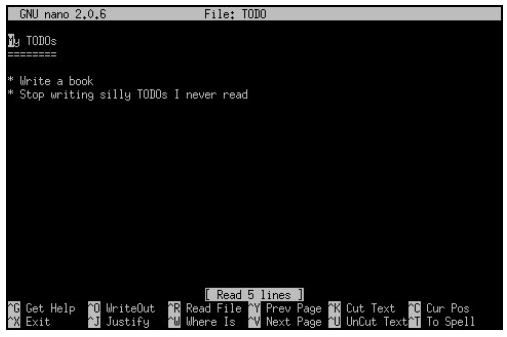
\includegraphics[scale=0.6]{scrn1}
\caption{Файл opentasks.txt, открытый в редакторе Nano в качестве рабочего документа}
\end{figure}

Первая строка отображает имя открытого файла, тогда как последние две строки набор команд, позволящих работать с файлом. Символ \verb|^| означает, что вам необходимо использовать клавишу Control (Ctrl) при использовании комбинации Ctrl+O, чтобы сохранить файл. Для выхода из редактора, нажмите Ctrl+X.

Некоторые текстовые файлы весьма чувствительны к новым строкам — это конфигурационные файлы — одни из наиболее важных. По умолчанию, при достижении боковой колонки nano преобразовывает строки автоматически. Чтобы «сказать» nano, что вам нужно сохранить их в исходном виде, добавьте аргумент \textbf{-w: «nano -w opentasks.txt»}. Рекомендуется при редактировании конфигурационных файлов.

\section{Просмотр текстовых файлов}

Если вы хотите просмотреть текстовый файл, но не желаете запускать текстовый редактор, можно использовать утилиты \textbf{cat} или \textbf{less}. Это также позволит вам просматривать содержимое файлов, не допуская случайных изменений.

С помощью cat вы «вываливаете» содержимое файла в терминал (или консоль). Если файл большой, текст пробежит очень быстро. Можно попытаться прокручивать его, используя комбинацию клавиш Shift+PgUp, одна длина этого буфера ограничена.

С помощью less, можно просматривать содержимое файла постранично. Команда less называется пейджером (pager), поддержимает прокрутку вверх / вниз (при помощи клавиш со стрелками или PgUp/PgDown), поиск определенного текста и т.д.

Использование утилиты \textbf{less} не ограничивается одним лишь просмотром содержимого текстовых файлов, она применяется и для man-страниц (о которых мы поговорим чуть позже в этой главе).

\vspace{-0.5cm}
\begin{table}[!h]
%\centering
\caption{Краткий список часто используемых комбинаций утилиты less}
\begin{tabular}{|m{7cm}|m{9.5cm}|}
\hline
	Прокрутить вниз на одну строку & Клавиши e, j <ввод> или со стрелкой вниз\\
\hline
	\small{Прокрутить выше на одну строку} & Клавиши y, k <ввод> или со стрелкой вверх\\
\hline
	Прокрутить вниз на одну строку & Клавиши f, <пробел> или PgDown\\
\hline
	\small{Прокрутить выше на одну строку} & Клавиши b или PgUp\\
\hline
	/<искомый текст> & Запрос <искомого текста> в начале, используйте «n» для подтверждения.\\
\hline
	h & Отобразить экранную справку\\
\hline
	?<искомый текст> & Запрос <искомого текста> в конце, используйте «?» для подтверждения.\\
\hline
\end{tabular}
\end{table}

Если вам интересно, имя \textbf{less} — это отсылка к старому, но всё ещё поддерживаемому пейджеру \textbf{more}. С помощью \textbf{more} вы также можете просматривать файлы постранично, однако он поддерживает только прокрутку вниз на одну строку (<ввод>) или на одну страницу (<пробел>). Таким образом, \textbf{less} больше\ldots чем \textbf{more}.

\section{Создание ссылок на файлы и каталоги}

Linux поддерживает два вида ссылок: символические и жесткие. Вам может быть любопытно, почему я рассказываю об этом во вводной главе о запущенном Linux. Что ж, потому, что символические ссылки довольно часто используются в Linux, тогда как вы обнаружите, что жесткие ссылки используются намного реже. На самом деле, ранее мы уже видели вывод команды, имеющей отношение к жестким ссылкам: взгляните на вывод команды \textbf{ls -l}.

\textit{Символические ссылки,} также известные как симлинки, просты для понимания. Это не существующие файлы, но ссылаются на них где либо в файловой системе. Они ссылаются на строку размещения, которая позволяет ссылке существовать, даже если файлы, к которым она обращается, (больше) не существуют. Например, у вас может быть символическая ссылка, указывающая на /home/swift/\break{}opentasks.txt, даже в том случае, если этот файл (больше) не существует.

\textit{Жесткие ссылки}, напротив, прямые. Они ссылаются на то же расположение на жестком диске, используемое в качестве точки назначения (через иноды), а файловая система не освобождает пространство, занятое им до тех пор, пока ссылки на это расположение не перестанут существовать. На самом деле, каждый файл, который вы видите в файловой системе, это ссылка на его расположение. Используя жесткие ссылки, можно создавать дполнительные ссылки.

Из-за своей технологии, такие ссылки обращаются только к файлу, расположенному на том же накопителе и не воспринимают каталоги. 
Чтобы создавать ссылки, используйте ln (жесткие ссылки) или ln -s (симлинки):

\vspace{3mm}
\begin{tcolorbox}
%\begin{lstlisting}
\$ ln имя\_файла\_назначения новое\_имя\_файла \\
\$ ln -s имя\_файла\_назначения новое\_имя\_файла
%\end{lstlisting}
\end{tcolorbox}

Благодаря им, вы можете управлять файлами намного легче. Например, у вас может быть важный текстовый файл, расположенный по адресу  ~/Documents/Work/\break{}Thesis/myThesis.txt, который ссылается на него из домашнего каталога пользователя (ссылка ~/myThesis.txt ведет на ~/Documents/Work/Thesis/MyThesis.txt) тем самым, не придется просматривать все каталоги каждый раз, когда нужно открыть или отредактировать файл. 

\section{Автодополнение для файлов и команд}

Эффективная возможность большинства командных интерпретаторов Linux - автодополнение для файлов и команд.

\sloppy К примеру, при редактировании файла под названием opentasks.txt, можно написать «nano o», а затем нажать клавишу <tab>. Если набранный текст «opentasks.txt» принадлежит файлу или каталогу, начинающемуся на букву «о», командный интерпретатор автоматически дополнит команду так, что она примет вид «nano opentask.txt». Если же имеется больше файлов или каталогов, начинающихся на «o», двойное нажатие клавиши <tab> позволит рассмотреть список претендентов на выбор.

То же верно и для команд. Если слово nano начинается на na (это не так, но предположим), то набрав его часть na и нажав клавишу <tab>, можно дополнить её остальной частью. Нажатие <tab> дважды выведет список всех совпадений не только для команд: 

\vspace{3mm}
\begin{tcolorbox}
\begin{lstlisting}
$ na<tab><tab>
namei		nautilus
nano		nasl
nasm		native2ascii
$ na
\end{lstlisting}
\end{tcolorbox}

\section{Переключение терминалов}

Одно из преимуществ Unix/Linux заключается в поддержке нескольких терминалов. Когда вы входите в систему, то обычно видите один из (виртуальных) терминалов так, словно он единственный. Можно переключаться с одного терминала на другой используя комбинацию Alt+F\#, где F\# - это F1, F2, … и другие клавиши. Если вы находитесь в графической сессии, следует использовать Crl+Alt+F\#. Графический дисплей расположен на первом терминале, который не может быть использован для входа (в большинстве случаев Alt+F7).

Поддержка нескольких терминалов позволяет вам входить в систему несколько раз и выполнять необходимые задачи параллельно, через различные терминалы. К примеру, при конфигурировании программы, удобно иметь её конфигурационный файл, открытым в одном терминале и саму программу, запущенной в другом. 

Подсказка: если вы работаете с командной строкой, то можете использовать команду \textbf{chvt} чтобы переключаться между терминалами: выполнение \textbf{chvt 2} переключает на второй терминал (имеет сходство с Alt+F2).

\section{Выход из сессии}

Чтобы выйти из существующей сессии, введите \textbf{enter} или нажмите Ctrl+d:

\vspace{3mm}
\begin{tcolorbox}
\begin{lstlisting}
captain@seaheaven ~ $ exit
This is seaheaven.homeworld (Linux x86_64 3.8.5) 22:30:00
seaheaven login:
\end{lstlisting}
\end{tcolorbox}

И наконец, если хотите выключить систему, сперва нужно стать суперпользователем. Вы можете сделать это, переключившись на другой терминал и войдя в систему как суперпользователь (root), но можете также использовать команду su. Эта команда попросит вас ввести пароль суперпользователя, после чего вы станете известным системе как пользователь с его привилегиями. 

\vspace{3mm}
\begin{tcolorbox}
\begin{lstlisting}
captain@seaheaven ~ $ su -
\end{lstlisting}
Password: (Введите пароль root)
\begin{lstlisting}
root@seaheaven ~ #
\end{lstlisting}
\end{tcolorbox}

Теперь, можно выполнить команду shutdown для немедленного выключения (-h) или перезагрузки (-r) системы:

\vspace{3mm}
\begin{tcolorbox}
\begin{lstlisting}
root@seaheaven ~ # shutdown -h now
\end{lstlisting}
\end{tcolorbox}

\section{Получение помощи}

В первое время Linux может казаться довольно сложным, поскольку утилиты, используемые новичками являются теми же, которые используются опытными пользователями. Новички не смогут понять  предназначение расширенных параметров этих утилит.  Лишь настольные книги, такие как эта, могут помочь пользователям найти свой путь, однако в то же время любой пользователь, будь то начинающий или опытный, нуждается в отправной точке информации. К счастью, существуют несколько ресурсов, к которым вы можете обратиться...

\subsection{Man-страницы}

Man страница, также называемая страницей с инструкцией доступна на системе Linux через команду man. Используя эту команду, вы можете получить информацию, объясняющую что она делает, какой синтаксис необходимо использовать, какие параметры она поддерживает и какие команды или файлы имеют к ней отношение. 

\section{Выключение}

\vspace{3mm}
\begin{tcolorbox}
\begin{lstlisting}
~$ man emerge
\end{lstlisting}
\end{tcolorbox}

Страница с инструкцией обычно структурирована следующим образом:

\begin{itemize}
	\item название команды с однострочным описанием
	\item синопсис команды, отображающий поддерживаемый командой синтаксис
	\item параметры команды с объяснением каждого из них
	\item дополнительная информация о команде, такая как, ограничения по использованию, поведение команды по умолчанию, 
	\item сведения об авторских правах и владельце
	\item другие связанные с этой страницы
\end{itemize}

Страницы с инструкциями прилагаются не только к командам, но и к файлам (конфигурационные или файлы устройств), системным вызовам или функциям библиотек (сведения, касающиеся программирования) и даже к стандартам и соглашениям. Эти разделы распределены по соответствующим секциям и соответственно пронумерованы:

\begin{enumerate}
	\item пользовательские команды
	\item системные вызовы
	\item функции библиотек
	\item специальные файлы (файлы устройств)
	\item форматы файлов и протоколы
	\item игры и развлекательные программы
	\item обзор, соглашения и различные разделы
	\item административные и привилегированные команды
\end{enumerate}

Для получения информации об этих разделах, откройте ознакомительную страницу к каждому из разделов. К примеру, ознакомительная страница к играм доступна по команде \textbf{man 6 intro}. Важно знать, какой раздел доступен, особенно если информация содержится в различных разделах под тем же названием. Например, passwd: имеется страница с инструкцией для команды \textbf{passwd} (\textbf{man 1 passwd}) и еще одна страница для файла passwd (\textbf{man 5 passwd}) Если ввести команду \textbf{man passwd}, то отобразится первый раздел или топик для этой страницы (в данном примере, первый раздел).

Попав на страницу с инструкцией, вы можете ориентироваться в ней, используя клавиши со стрелками вверх/вниз  и PgUp//PgDown. Также можно выполнить поиск по конкретному запросу (нажмите / и введите искомое слово) и многое другое. Полное объяснение всех команд просмотрщика инструкций (который во многих системах является утилитой less) можно получить, нажав 'h'.

Чтобы завершить просмотр страницы, нажмите 'q'.

Если вы уверены, что страница с инструкцией имеется где-то в системе, но не знаете ее название, можно использовать команду apropos (которая эквивалентна команде man -k). Если передать ключевое слово команде, она отобразит список страниц, связанных с этим запросом. Чтобы создать базу данных, сперва необходимо запустить команду makewhatis. На большинстве система она выполняется в фоновом режиме ежедневневно, согласно запланированной задаче.  

\vspace{3mm}
\begin{tcolorbox}
\begin{lstlisting}
~ apropos ebuild 
\end{lstlisting}
\end{tcolorbox}

\subsection{Информационные страницы}

Другая справочная утилита на вашей системе — это справочная система info. Инструмент info позволяет просматривать info-страницы в иерархическом представлении (переход к предыдущей/следующей секции, выше, …) а так же с использованием гиперссылок (выбор топика на странице для перехода к разделу соответствующего топика).

Давайте взглянем на info-страницу GCC:

\vspace{3mm}
\begin{tcolorbox}
\begin{lstlisting}
~$ info gcc
...
File: gcc.info,
 Node: Top,
 Next: G++ and GCC,
 Up: (DIR)
Introduction
************
\end{lstlisting}
This manual documents how to use the GNU compilers, as well as their
features and incompatibilities, and how to report bugs. It corresponds
to GCC version 4.1.2. The internals of the GNU compilers, including
how to port them to new targets and some information about how to write
...

\end{tcolorbox}

В начале страницы можно обнаружить последовательность документов (тут нет предыдущего или следующего раздела, так как это первая страница). Следующий топик (к которому можно перейти нажатием n) называется «G++ и GCC».

В самом тексте вы найдете куски текста, разделенного по двум колонкам:

\vspace{3mm}
\begin{tcolorbox}
\begin{lstlisting}
* G++ and GCC:: You can compile C or C++ programs.
* Standards:: Language standards supported by GCC.
* Invoking GCC:: Command options supported by `gcc'.
* C Implementation:: How GCC implements the ISO C specification.
* C Extensions:: GNU extensions to the C language family.
* C++ Extensions:: GNU extensions to the C++ language.
* Objective-C:: GNU Objective-C runtime features.
\end{lstlisting}
\end{tcolorbox}

Являясь ссылками, они позволяют вам перемещаться по топикам. Наведите курсор на надпись «Invoking GCC» и нажмите клавишу ввода:

\vspace{3mm}
\begin{tcolorbox}
%\begin{lstlisting}
File: gcc.info, Node: Invoking GCC, Next: C Implementation, Prev: Standards,
3 GCC Command Options
*********************
When you invoke GCC, it normally does preprocessing, compilation,
assembly and linking. The "overall options" allow you to stop this
process at an intermediate stage. For example, the `-c' option says
not to run the linker. Then the output consists of object files output
by the assembler.
%\end{lstlisting}
\end{tcolorbox}

Теперь вы находитесь в блоке под названием «Invoking GCC». Следующий раздел - «C Implementation», а предыдущим (p) был «Standards», и если вы пройдете дальше (\textbf{u}), то снова окажетесь в самом начале документа.

Информационные страницы часто используются  различными проектами GNU (такими как GCC). Тем не менее, страницы с инструкциями более популярны, возможно, поскольку разработчики находят их простыми для написания. 

\section{Краткая справка по синтаксису}

Если вы не ищете объяснения команды, но хотите знать синтаксис, большинство команд предоставляет краткую справку при помощи аргументов

\vspace{3mm}
\begin{tcolorbox}
-h или --help.
\begin{lstlisting}
$ man -h
man, version 1.6e
usage: man [-adfhktwW] [section] [-M path] [-P pager] [-S list]
[-m system] [-p string] name ...
a : find all matching entries
c : do not use cat file
d : print gobs of debugging information
D : as for -d, but also display the pages
f : same as whatis(1)
h : print this help message
k : same as apropos(1)
K : search for a string in all pages
t : use troff to format pages for printing
\end{lstlisting}
\end{tcolorbox}
\vspace{3mm}
\begin{tcolorbox}
\begin{lstlisting}
w : print location of man page(s) that would be displayed
(if no name given: print directories that would be searched)
W : as for -w, but display filenames only
C file : use `file' as configuration file
M path : set search path for manual pages to `path'
P pager : use program `pager' to display pages
S list : colon separated section list
m system : search for alternate system's man pages
p string : string tells which preprocessors to run
e - [n]eqn(1) p - pic(1)
t - tbl(1) g - grap(1)
\end{lstlisting}
r - refer(1) v — vgrind (1)
\end{tcolorbox}


\section{Документация, предоставляемая пакетом}

Некоторые пакеты предоставляют больше документации в виде руководств (в форматах HTML, PDF и др.), файлов README и т.д. Вы можете найти ее по адресу /usr/share/doc. В Gentoo Linux документы упакованы с помощью bzip или gzip (две хорошо известные в мире Unix утилиты архивации). Чтобы  просмотреть их, необходимо сперва распаковать в область на жестком диске, где имеются привилегии для записи.

Допустим, пакет zip содержит документ, объясняющий какой алгоритм использует утилита для (раз)архивирования данных:

\vspace{3mm}
\begin{tcolorbox}
\begin{lstlisting}
$ cd /usr/share/doc/zip-*
$ ls
algorith.txt.bz2 BUGS.bz2 CHANGES.bz2 MANUAL.bz2
README.bz2 timezone.txt.bz2 txtvsbin.txt.bz2 WHATSNEW.bz2
WHERE.bz2 ziplimit.txt.bz2
$ bunzip2 -c algoritm.txt.bz2 > ~/algorithm.txt
\end{lstlisting}
\end{tcolorbox}

Полученный файл, algorithm.txt, можно найти в каталоге ~ (~ - аббревиатура домашнего каталога текущего пользователя). В этом случае, файл является обычным текстовым файлом, который можно просмотреть с помощью команды less, также используемой для man-страниц.

В вышеуказанном примере используется перенаправление: вывод команды  (\textbf{bunzip2 -c algorithm.txt.bz2}) не показывается на экране, но перенаправляется в файл (\textbf{algorithm.txt}). Но об этом мы поговорим позже.

Также возможно чтение (сжатого) файла, используя команду bzless:

\vspace{3mm}
\begin{tcolorbox}
\begin{lstlisting}
$ bzless algorithm.txt.bz2
\end{lstlisting}
\end{tcolorbox}

\section{Онлайн-документация}

Многие проекты имеют богатую документацию. Советуем вам внимательно взглянуть на веб-сайты проектов или поискать в Интернете доступные руководства и книги. Иногда, лучшая документация может быть написана не самим проектом, но его пользователями.

\newpage
{\color{white}\section{Упражнения}}
\begin{tcolorbox}[title=\textbf{Упражнения}, colback=yellow!14!white, colframe=red!75!white]
\begin{enumerate}
	\item Попробуйте организать ваш домашний каталог по логическим разделам. К примеру, создайте каталоги, где вы будете хранить личные документы, изображения, документы по работе и просто временные документы. 
	\item 2. В общем, системы Unix/Linux предлагают вам четыре метода архивации (сжатия). Системы Unix/Linux используют Gzip или BZip2 вместе с tar, тогда как лишь Zip — хорошо известный формат в операционных системах Microsoft Windows. Каким образом «tar» используется с gzip/bzip2? Что же такое четвертый метод архивации?
	\item Как уже было упомянуто, системы Unix/Linux не имеют функциональности, позволяющей обратить изменения: когда вы удаляете файл, он удаляется. Однако, из-за особенности техники удаления файлов (фактически удаляется лишь ссылка к файлу, однако его содержимое остается на диске до перезаписи) существуют инструменты, которые могут помочь вам вернуть удаленные файлы. Попробуйте найти несколько примеров подобных утилит восстановления для Linux.
\end{enumerate}
\end{tcolorbox}

\phantom{}
\begin{tcolorbox}[title=\textbf{Дальнейшие ресурсы}, colback=yellow!14!white, colframe=red!75!blue]
\begin{itemize}
	\item[+] Introduction to Linux, A Hands-On Guide [\href{http://www.tldp.org/LDP/intro-linux/html/index.html}{http://www.tldp.org/LDP/intro-linux/html/index.html}]
	\item[+] by Machtelt Garrels (also available as PDF [\href{http://www.tldp.org/LDP/intro-linux/intro-linux.pdf}{http://www.tldp.org/LDP/intro-linux/intro-linux.pdf}]
\end{itemize}
\end{tcolorbox}

%%% Глава 5. Файловая система Linux %%%
\chapter{Файловая система Linux}

\section*{Введение}

Файловая система Linux имеет вид иерархически структурированного дерева, где каждая область имеет определённое значение. Структура файловой системы  определена в стандарте иерархии файловой системы, описание которого вы можете найти в этой главе. Тем не менее, всё больше дистрибутивов вносит изменения в структуру своих файловых систем (но и в их содержимое), поэтому стандарту необходимо обновляться. В каком случае настройка отличается от текущего стандарта, я расскажу далее в этой главе.

Конечно, файловая система всегда хранится на носителе (будь то жесткий диск, компакт-диск, или фрагмент памяти); Каким образом эти носители связаны с ней и как Linux отслеживает их — это всё также будет разъяснено в этой главе.

\section{Структура}

Файловая система имеет древовидную структуру. Её корень, по случайному совпадению, называется корнем файловой системы, однако представляется выше всех остальных её ветвей и распознается по символу косой черты «/». Это наивысшая точка размещения, куда вы можете попасть. Тут почти всегда располагаются только каталоги:

\vspace{3mm}
\begin{tcolorbox}
\begin{lstlisting}
~$ cd /
~$ ls -F
bin/	home/	opt/	srv/	var/
boot/	lib/	proc/	sys/
dev/	media/	root/	tmp/
etc/	mnt/	sbin/	usr/
\end{lstlisting}
\end{tcolorbox}

Команда \textbf{ls -F} выводит содержимое корневой точки размещения, но добавляет к именам специальных файлов дополнительные символы. К примеру, добавляет к   каталогам символ «/», символическим ссылкам символ «@» и исполняемым файлам символ «*». Преимущество, на данной момент в этой книге, в том, что вы сможете легко различать типы файлов, которые увас есть. По умолчанию, для команды ls в Gentoo активен цветной режим, который подсказывает вам предназначение каждого файла с помощью расцветки. Тем не менее, нспользование обозначений с символами намного разумнее для иллюстрации в книгах.

Популярный способ представления файовой системы в виде древа. В данном примере показан верхний уровень:

\vspace{3mm}
\begin{tcolorbox}
%\begin{lstlisting}
\begin{tabular}{cc}
	/ & +-bin/\\
	+-boot/ & +-dev/\\
	+-etc/ & +-lib/\\
	+-home/ & +-media/\\
	+-mnt/ & +-opt/\\
	+-proc/ & +-root/\\
	+-sbin/ & +-srv/\\
	+-sys/ & +-tmp/\\
	+-usr/ & `-var/\\
\end{tabular}
%\end{lstlisting}
\end{tcolorbox}

Чем больше переходов, тем больше становится древо, и в скором времени станет труднее отобразить структуру в одиночном виде. Древовидный формат - всё ещё хороший способ представления файловой системы, поскольку он представляет её точно так, как вы видите.

\vspace{3mm}
\begin{tcolorbox}
\begin{lstlisting}
/
+-	bin/
+-	...
+-	home/
|	=-	thomas/
|	|	+-	Documents/
|	|	+-	Movies/
|	|	+-	Music/
|	|	+-	Pictures/	<-- You are here
|	|	|	'-	Backgrounds/
|	|	'-	opentasks.txt
|	+-	jane/
|	'-	jack/
+-	lib/
+-	...
'-	var/
\end{lstlisting}
\end{tcolorbox}

Ранее мы уже освещали моменты, касающиеся навигации по древу вкратце: предположим, вы находитесь по адресу /home/thomas/Pictures. Чтобы пройти ещё дальше (в каталог Backgrounds) необходимо выполнить команду «\textbf{cd Backgrounds}». Чтобы перейти назад (в /home/thomas) следует выполнить «\textbf{cd ..}» (.. обозначает родительский каталог).

Перед тем как объяснять различные размещения, давайте сперва рассмотрим, как файловая система располагается или хранится на одном носителе (или более одного)\ldots

\section{Монтирование файловых систем}

Предположим, что корень файловой системы у вас расположен на одном разделе, а все 'пользовательские' файлы на другом. Это могло бы означать, что / всё что ниже по иерархии находится на одном разделе, за исключением точки /home и всего что в ней, которая расположена на втором разделе.

\begin{figure}[!t]
\centering
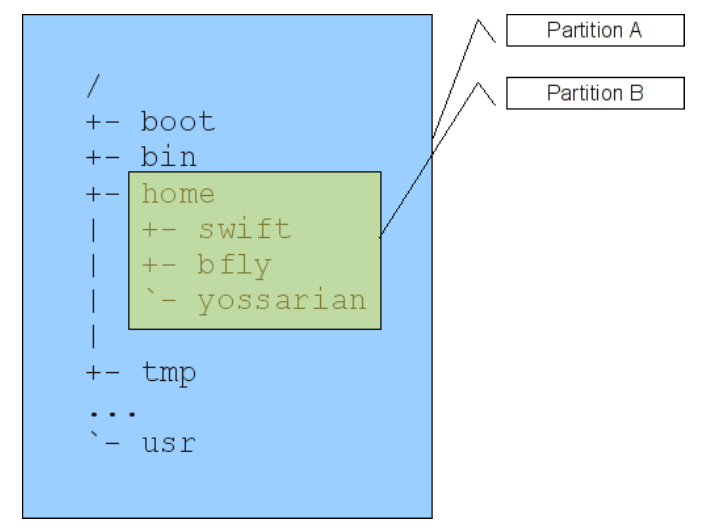
\includegraphics[scale=0.6]{scrn2}
\caption{Два раздела, используемые как части структуры файловой системы}
\end{figure}

Выполнение монтирования требует от вас указать размещение файловой системы для точки монтирования (например, точка монтирования — это /home), в которой каждый файл в действительности находится в другом месте (в этом примере, всё что исходит от родительского каталога /home, находится на втором разделе).  Монтируемому разделу не нужно знать куда он примонтирован. В действительности, он не знает этого. Вы можете монтировать подкаталоги пользовательского каталога в /home (что предпочтительнее), однако лучше всего монтировать их в  /srv/export/systems/remote/disk/users. Разумеется, причина по который вы должны сделать так же — мой пример, но можно сделать это и по-своему.

Команда mount, запущенная без каких-либо аргументов покажет список примонтированных файловых систем: 

\vspace{3mm}
\begin{tcolorbox}
\begin{lstlisting}
$ mount
 /dev/sda8 on / type ext3 (rw,noatime)
 proc on /proc type proc (rw) sysfs on /sys type sysfs (rw,nosuid,nodev,noexec,relatime)
 udev on /dev type devtmpfs (rw,nosuid,relatime,size=10240k,mode= devpts
 on /dev/pts type devpts (rw,nosuid,noexec,relatime,gid=5,mode 
 /dev/sda7 on /home type ext3 (rw,noatime) 
 none on /dev/shm type tmpfs (rw) /dev/sda1 on
 /mnt/data type ext3 (rw,noatime) 
 usbfs on /proc/bus/usb type usbfs (rw,noexec,nosuid,devmode=0664,devgi
\end{lstlisting}
\end{tcolorbox}

 
Вышеприведенный пример содержит большое количество разных файловых систем, о которых мы ещё ничего не знаем, и говорит нам, что файловая система может бть представлена в следующем виде:

\vspace{3mm}
\begin{tcolorbox}
\begin{lstlisting}
/       (on /dev/sda8)
+-  ...
+-  dev/    (special: "udev")
|   +- pts  (special: "devpts")
|   `- shm  (special: "none")
+-  proc/   (special: "proc")
|   `- bus/
|    `- usb/ (special: "usbfs")

+-  sys/    (special: "sys")
+-  home/   (on /dev/sda7)
`-  mnt/
     `- data/ (on /dev/sda1)
\end{lstlisting}
\end{tcolorbox}

Игнорируя специальные точки монтирования, можно увидеть корень файловой системы на устройстве /dev/sda8. С другой стороны, /home, файловая система этой точки хранится на /dev/sda7, а данные /mnt/data, в свою очередь в /dev/sda1. Позже мы подробнее разберем синтаксис специфичных устройств.

Концепция монтирования позволяет программам знать, где структурированы ваши данные. С точки зрения приложения (или пользователя), файловая система является единым древом. Под «капотом» же, она может состоять из одного раздела, дюжины разделов, сетевого хранилища, съемных носителей и др.

\section{Файловые системы}

Каждый носитель содержит файлы, которые структурированных внутренне. То, как выглядит их структура, является частью используемой файловой системы. Пользователи Windows могут вспомнить, что в самом начале, перед тем как мигрировать на одну из множества ревизий NTFS, в Microsoft Windows применялись файловые системы FAT16 и позднее FAT32. Подобно этому примеру, Linux также имеет свои файловые системы.

Однако система не требует, чтобы все разделы содержали одну из возможных файловых систем (как например в упомянутой выше системе от Microsoft «поддерживается только NTFS»): до тех пор, пока она понимает их, а используемая файловая система поддерживает такие возможности, как права владельца и разрешения, вы вольны выбирать любую из них. В действительности, множество дистрибутивов имеет установщик, предлагающий выбрать одну из файловых систем. Следующий список — лишь небольшой, но вкратце описывающий наиболее популярные из файловых систем с перечислением их преимуществ и недостатков...

\begin{itemize}
  \item Файловая система \textit{ext2} — старая, но всё ещё используемая в Linux. Она представляет собой расширенную файловую систему второй версии и довольно проста. Она использовалась почти с момента появлдения Linux на свет и достаточно устойчива к фрагментации данных — что тем не менее, верно почти для всех файловых систем Linux. Однако медленно замещается журналируемыми.
  \item Файловая система \textit{ext3} — усовершенствованная версия ext2, кроме других возможностей имеет концепцию журналирования.
  \item Файловая система \textit{ext4} — усовершенствованная версия ext3, кроме  всего прочего имеет поддержку очень больших систем/файлов, экстентов (смежные физические блоки), предварительного выделения, отложенного выделения и др. Ext4 является обратно совместимой с ext3 до тех пор, пока не используются экстенты.  Неоднократно замечена как файловая система, выбираемая по умолчанию среди большинства администраторов и дистрибутивов.
  \item Файловая система \textit{reiserfs} разработана с нуля. Также предоставляет журналирование, но в основном сфокусирована на производительности. Предоставляет быстрый доступ к точке размещения с тысячами файлов (ext2 и ext3 в подобной ситуации достаточно медленные), экономит объем занимаемого пространства для небольших файлов (некоторые другие файловые системы резервируют весь блок для каждого файла, тогда как reiserfs способен разделять блоки с несколькими файлами, делая их общими). Несмотря на это была популярной несколько лет назад, в те годы ей не хватало поддержки (губительные ошибки оставались незамеченными некоторое время) и она реже предлагалась дистрибутивами. Её наследница, reiser4, всё ещё находится на раннем этапе развития, и вследствие ареста главного разработчика Ганса Рейзера, не слишком активно  разрабатывалась.
  \item Файловая система btrfs выглядит многообещающей. Нацелена на большие объемы данных, объединение нескольких устройств, снапшоты и многое другое. Несмотря на то, что в первую очередь предназначалась для использования на предприятиях, она также предлагает интересные возможности и для домашних пользователей, такие как увеличение или уменьшение размера на лету (на уровнях файловой системы и хранилища), резервирование объектного уровня, прозрачную компрессию и клонирование.
  \item Файловая система \textit{xfs} представляет собой высокопроизводительное решение с поддержкой журналирования, готовое для применения на предприятиях. Предлагает высокую параллельную пропускную способность, в связи с чем является распространенным выбором среди предприятий.
  \item Файловая система \textit{zfs} является многофункциональной и предлагает контрольное суммирование на блочном уровне, компрессию, снапшоты, возможность «копирования на лету», дедупликацию, очень большие тома, удалённую репликацию и многое другое. Ранее была портирована с ОС (Open)Solaris на Linux, где и обрела своё место.
\end{itemize}

\textit{Файловая система} отслеживает операции с записью файлов, производя метки (о добавлении новых файлов или изменении их содержимого) в свой журнал перед выполнением соответствующих операций. Затем выполняет запись данных на самой файловой системе, после чего удаляет метку об этом. Данный набор операций обеспечивает способность восстановить целостность файловой системы с помощью проверки журнала или удаления незавершенной записи в том случае, если операции над файловой системой внезапно прерываются (к примеру, из-за сбоя питания): таким образом она всегда находится в консистентном состоянии.

Обычно нет возможности переключаться между файловыми системами (за исключением ext2<>ext3), однако большинство из них достаточно развиты, поэтому вам не нужно паниковать по поводу выбора «правильной файловой системы».

Теперь, если мы взглянем на следующий вывод команды mount, то заметим, что часть строки говорит нам о том, какого «типа» точка монтирования. Следовательно, это и есть тип файловой системы, используемой для отдельного монтирования.

\vspace{3mm}
\begin{tcolorbox}
\begin{lstlisting}
$ mount
rootfs on / type rootfs (rw) 
sysfs on /sys type sysfs (rw,seclabel,relatime)
selinuxfs on /sys/fs/selinux type selinuxfs (rw,relatime) 
/dev/md3 on / type ext4 (rw,seclabel,noatime,no 
/dev/md4 on /srv/virt type ext4 (rw,noatime,data=ordered
proc on /proc type proc (rw,nosuid,nodev,noexec 
tmpfs on /run type tmpfs (rw,rootcontext=system_
udev on /dev type devtmpfs (rw,seclabel,nosuid,relative 
/dev/mapper/volgrp-nfs on /srv/nfs type ext4 (rw,noatime,data=journal
/dev/mapper/volgrp-usr on /usr type ext4 (rw,noatime,data=journal 
/dev/mapper/volgrp-home  on /home type ext4 (rw,noatime,nosuid,node
/dev/mapper/volgrp-opt on /opt type ext4 (rw,noatime,data=journal
/dev/mapper/volgrp-var on /var type ext4 (rw,noatime,data=journa
/dev/mapper/volgrp-vartmp on /var/portage type ext4 (rw,noatime,data=ordered
mqueue on /dev/mqueue type mqueue (rw,seclabel,nosuid,nod 
devpts on /dev/pts type devpts (rw,seclabel,nosuid,noe
shm on /dev/shm type tmpfs (rw,seclabel,nosuid,nod
securityfs on /sys/kernel/security type securityfs (rw,nosuid,nodev,noexec
debugfs on /sys/kernel/debug type debugfs (rw,nosuid,nodev,noexec
none on /selinux type selinuxfs (rw) 
tmpfs on /var/tmp type tmpfs (rw,nosuid,noexec,nodev 
tmpfs on /tmp type tmpfs (rw,nosuid,noexec,nodev
rc-svcdir on /lib64/rc/init.d type tmpfs (rw,nosuid,nodev,noexec 
binfmt_misc on /proc/sys/fs/binfmt_misc type binfmt_misc (rw,nodev,noexec,nosuid 
rpc_pipefs on /var/lib/nfs/rpc_pipefs type rpc_pipefs (rw)
nfsd on /proc/fs/nfsd type nfsd (rw,nodev,noexec,nosui
\end{lstlisting}
\end{tcolorbox}

Как вы видите, все разделы (строки неспециального назначения) имеют тип ext4. Но что если выбрать другие файловые системы?

Proc — файловая система, которой не существует на устройстве, однако она явлется чем-то наподобие врат или шлюза доступа к ядру Linux. Всё, что вы видите ниже по иерархии /proc — это то, что ядро отображает, когда  просматривается её содержимое. Это способ коммуникации с ядром (и наоборот), использующий очень простой интерфейс: чтение и запись файлов, что-то, что хорошо поддерживается.

Я расскажу вам о /proc больше в этой главе.

\begin{itemize}
  \item proc известен как псевдофайловая система: она не содержит реальных файлов, но хранит в себе данные, касающиеся рабочих процессов.
  \item sysfs - специальная система, такая как proc: она не существует на устройстве, и тоже является подобием шлюза доступа к ядру Linux. Отличается от proc тем, как спроектирована и структурирована: sysfs более структурирована и рассчитана на компьютерный разбор файлов и директорий, тогда как proc имеет структуру и предназначение для более удобного их чтения или записи пользователем.
  \begin{itemize}
    \item В перспективе proc исчезнет (однако, ключевого срока не существует, поскольку множество людей предпочитает простой способ с использованием /proc, что даёт  им необходимые данные) и будет заменена файловой системой sysfs.
  \end{itemize}
  \item tmpfs — временная файловая система, содержимое которой хранится в памяти вместо постоянного хранилища. Таким образом, она используется довольно часто (оперативная память намного быстрее даже самых производительных SSD и жестких дисков). Скажем так, обычно, tmpfs может выгружать страницы памяти в область подкачки, что незамедлительно делает эту часть файловой системы tmpfs медленней (так как  перед использованием они должны считываться с диска).
  \begin{itemize}
    \item В Linux tmpfs используется для таких нужд, как общая память в /dev/shm и /tmp.
  \end{itemize}
  \item Файловая система devtmpfs имеет сходство с tmpfs, но содержит файлы устройств, управляемых ядром. Она воплощает в жизнь возможность запуска и контроля важных файлов устройств до передачи их udev (менеджеру устройств).
  \item devpts — еще одна псевдофайловая система, подобная proc и tmpfs. Содержит файлы устройств, используемых для эмуляции терминала (например, предоставляет доступ к консоли в графической среде при помощи xterm, uterm, eterm или другой программы, эмулирующей терминал). Ранее, упомянутые файлы устройств создавались статически, из-за чего большинство дистрибутивов приходилось снабжать большим количеством файлов устройств, эмулирующих терминал (посколько было затруднительным знать, сколько таких эмуляций пользователь мог бы запустить со временем). Чтобы лучше управлять ими, была разработана псевдофайловая система, которая создает и уничтожает файлы устройств по мере необходимости.
  \item usbfs также является псевдофайловой системой и может быть сравнима с devpts. Также содержит файлы, которые создаются в момент подключения или извлечения устройств USB. Тем не менее, в отличие от dvpts вместо файлов устройств она создает псевдофайлы, которые могут быть использованы для взаимодействия с устройством USB.
  \begin{itemize}
    \item Так как большинство из них является стандартными устройствами USB (принадлежащие определенным классам, как стандартные устройства хранения USB) для Linux разработан фреймворк, позволяющий программам работать с устройствами USB, основываясь на их характеристиках посредством файловой системы usbfs.
  \end{itemize}
  \item selinuxfs — еще одна псевдофайловая система, представляющая подсистему SELinux в ядре Linux. Используется библиотеками SELinux для взаимодействия с сервером безопасности SELinux, запрашивающий имеющиеся политики SELinux и многое другое. Эта файловая система не монтируется на системах Linux, в которых не включена подсистема SELinux.
  \item mqueue — псевдофайловая система, используемая для поддержки межпроцессных сообщений (очередь сообщений POSIX)
  \item $binfmt_misc$ — псевдофайловая система, используемая для регистрации исполняемых файлов. Посредством binfmt ядро Linux способно выполнять произвольные форматы исполняемых файлов, распознавая зарегистрированные исполняемые форматы и передавая их приложениям, находящимся в пользовательском пространстве. 
\end{itemize}

Существует множество специальных файловых систем (некоторые из них даже упомянуты выше в выводе команде mount), однако я оставлю это для интересующегося читателя, который найдет больше информации об этих файловых системах.

\section{Разделы и диски}

Каждое устройство, подключенное к оборудованию (кроме сетевого интерфейса) и доступное в Linux, представляется в виде файлов устройств, размещенных в /dev. Разделы и диски — не исключение. Возьмем к примеру жёсткий диск Serial ATA.

Драйвер диска SATA использует внутренний слой SCSI для отображения и доступа к данным. Собственно, устройство SATA представляется как устройство SCSI. Первый диск SATA в вашей системе отображается как устройство /dev/sda, а его первый раздел станет /dev/sda1. Вы можете расшифровать sda1 как «1-ый раздел (1) на первом (а) устройстве scsi (sd)».

\vspace{3mm}
\begin{tcolorbox}
\begin{lstlisting}
~$ ls -l /dev/sda1
brw-rw---- 1 root disk 8, 1 Nov 12 10:10 /dev/sda1
\end{lstlisting}
\end{tcolorbox}

Обычный диск типа ATA (или DVD-ROM) отобразится как /dev/hda (сокращение hd означало жёсткий диск, но теперь применяется для распознавания устройства ATA).

\vspace{3mm}
\begin{tcolorbox}
\begin{lstlisting}
$ ls -l /dev/hda
brw-rw---- 1 root cdrom 3, 0 Apr 23 21:00 /dev/hda
\end{lstlisting}
\end{tcolorbox}

В стандартной инсталляции Gentoo, менеджер устройств (называется udev) создает файлы устройств, обнаруженных оборудованием. К примеру, в моей системе, разделы первого устройства SATA могут быть представлены в следующем виде:

\vspace{3mm}
\begin{tcolorbox}
\begin{lstlisting}
$ ls -l /dev/sda*
brw-r----- 1 root disk 8, 0 Sep 30 18:11 /dev/sda
brw-r----- 1 root disk 8, 1 Sep 30 18:11 /dev/sda1 
brw-r----- 1 root disk 8, 2 Sep 30 18:11 /dev/sda2
brw-r----- 1 root disk 8, 5 Sep 30 18:11 /dev/sda5 
brw-r----- 1 root disk 8, 6 Sep 30 18:11 /dev/sda6 
brw-r----- 1 root disk 8, 7 Sep 30 18:11 /dev/sda7 
brw-r----- 1 root disk 8, 8 Sep 30 18:11 /dev/sda8
\end{lstlisting}
\end{tcolorbox}

Внутри каталога /dev также находятся символические ссылки (указатели) на файлы устройств, которые могут использоваться для идентификации разделов или дисков другим способом. К примеру, чтобы отобразить список блочных устройств, используя их UUID (Универсальный Уникальный Идентификатор):

\vspace{3mm}
\begin{tcolorbox}
\begin{lstlisting}
$ ls -l /dev/disk/by-uuid
total 0
lrwxrwxrwx. 1 root root 10 Dec 16 20:01 1628b93d-3448-4b8c-b72b-1d68e89bd2fa -> 
lrwxrwxrwx. 1 root root 10 Dec 16 20:01 5550c45f-9660-44f2-8e86-05a612d028a3 ->
lrwxrwxrwx. 1 root root 10 Dec 16 20:01 77eb40be-f571-49c6-bbb0-a12677615fe3 ->
lrwxrwxrwx. 1 root root 10 Dec 16 20:01 9644f675-6eaf-4974-9e1a-0b8eafa931ae ->
lrwxrwxrwx. 1 root root 10 Dec 16 20:01 9beda062-6e15-4323-9ad1-53b6a9e39676 -> 
lrwxrwxrwx. 1 root root 10 Dec 16 20:01 9e7a1178-b0ad-4cd8-8977-a471a5d2b797 -> 
lrwxrwxrwx. 1 root root 9 Dec 16 20:01 b06fa545-0d5a-4c9a-97cb-83b4e1799f9a -> 
lrwxrwxrwx. 1 root root 10 Dec 16 20:01 b80c76a3-d52f-4006-9bf5-62f4d7edc791 -> 
lrwxrwxrwx. 1 root root 10 Dec 16 20:01 bdb15de1-3430-47b4-9e63-ee58557f1d17 ->
lrwxrwxrwx. 1 root root 9 Dec 16 20:01 c44503ce-e52e-452c-b4bc-767ddd1d3b27 ->
lrwxrwxrwx. 1 root root 9 Dec 16 20:01 d8a2bb27-15da-49bb-b205-3160c307835c ->
\end{lstlisting}
\end{tcolorbox}

Преимущество использования этих UUID заключается в своеобразной идентификации раздела или диска. Если диски являются многофункциональными или мы говорим о съёмных устройствах, то используя UUID мы можем знать, что смотрим на правильный раздел (и не на другой диск, который, например, назван /dev/sda2).

\section{Команда 'mount' и файл fstab}

Монтирование носителя с файловой системой выполняется командой mount. Чтобы производить это действие достаточно хорошо, необходима некоторая информация, такая как точка монтирования, тип файловой системы, устройства и дополнительные параметры монтирования.

К примеру, команда mount, которая монтирует устройство /dev/sda7, содержащее файловую систему ext3 в точку /home, выглядит так:

\vspace{3mm}
\begin{tcolorbox}
\begin{lstlisting}
# mount -t ext3 /dev/sda7 /home
\end{lstlisting}
\end{tcolorbox}

Также можно увидеть, что это действие напоминает «прикрепление» определённого устройства к какой-либо области файловой системы, что эффективно расширяет её большим количеством файлов, директорий и прочих данных.

Однако, если в системе имеется несколько разных разделов, необходимость вводить команды снова и снова может показаться глупой шуткой. Это одно из причин наличия в Linux специального файла, содержащего список файловых систем. Называется он /etc/fstab и содержит всю информацию, которая может быть необходима, чтобы успешно монтировать устройство. Пример содержимого файла fstab приведен ниже:

\vspace{3mm}
\begin{tcolorbox}
\begin{lstlisting}
/dev/sda8 /           ext4    defaults,noatime      0 0
/dev/sda5 none        swap    sw                    0 0
/dev/sda6 /boot       ext4    noauto,noatime        0 0
/dev/sda7 /home       ext4    defaults,noatime      0 0
/dev/sdb1 /media/usb  auto    user,noauto,gid=users 0 0
\end{lstlisting}
\end{tcolorbox}

Структура файла следующая:
\begin{enumerate}
  \item Устройство, предназначенное для монтирования (также подерживаются метки, но об этом мы поговорим позже)
  \item Размещение монтируемого устройства (точка монтирования)
  \item Тип файловой системы или auto (автоматический), если вы хотите, чтобы Linux автоматически определял её
  \item Дополнительные параметры (используйте «defaults», если не нуждаетесь в какой-либо специфичной опции), такие как «noatime» (не регистрировать время доступа к файловой системе для улучшения её производительности) и «users» (позволять обычным пользователям монтировать или размонтировать устройство)
  \item Номер дампа (можно оставить 0)
  \item Порядок проверки файлов (также можно оставить 0)
\end{enumerate}

Благодаря этому файлу, предыдущий пример с командой mount больше не требуется (так как монтирование выполняется автоматически), однако в том случае, если операция монтирования ещё не выполнена, команда упрощается до:

\vspace{3mm}
\begin{tcolorbox}
\begin{lstlisting}
# mount /home
\end{lstlisting}
\end{tcolorbox}

Если вам когда-либо потребуется удалить носитель из системы, используйте команду umount:

\vspace{3mm}
\begin{tcolorbox}
\begin{lstlisting}
# umount /home
\end{lstlisting}
\end{tcolorbox}

Это представляет особый интерес в случае со съемными носителями: если  необходимо получить доступ к носителю CD или DVD (или даже к USB-накопителю), перед этим сперва следует монтировать носитель с файловой системой. Аналогичным образом,перед удалением устройства из системы, его сперва необходимо отмонтировать:

\vspace{3mm}
\begin{tcolorbox}
\begin{lstlisting}
# mount /media/dvd
\end{lstlisting}
\end{tcolorbox}

(Устройство DVD теперь примонтировано и доступно)

\vspace{3mm}
\begin{tcolorbox}
\begin{lstlisting}
# umount /media/dvd
\end{lstlisting}
\end{tcolorbox}

(Устройство DVD теперь более не доступно в файловой системе и может быть извлечено из лотка).

Разумеется, современные операционные системы Linux снабжены инструментами, которые автоматически монтируют устройства для доступа по файовой системе и отмонтируют при их извлечении. По умолчанию, Gentoo Linux не предлагает их (их следует установить самостоятельно).

\section{Размещение раздела подкачки}

У вас есть (или возможно будет) раздел, выделенный специально для постраничной подкачки: Linux использует этот раздел, в нем при недостатке физической памяти хранятся данные обо всех запущенных процессах (и их ресурсах). Когда это происходит, операционная система начинает помещать эти данные (которые, возможно, не будут использованы в скором времени) на диск, освобождая физическую память.

Этот раздел такой же как и другие, однако вместо обычной используемой пользователями файловой системы, он содержит свою особенную для нужд памяти и опознается в таблице разделов как раздел подкачки.

\vspace{3mm}
\begin{tcolorbox}
\begin{lstlisting}
# fdisk -l /dev/sda
Disk /dev/sda: 60.0 GB, 60011642880 bytes
255 heads, 63 sectors/track, 7296 cylinders
Units = cylinders of 16065 * 512 = 8225280 bytes
Disk identifier: 0x8504eb57

Device Boot 	Start 	End	Blocks		Id 	System
/dev/sda1* 	1 	1275 	10241406 	83 	Linux 
/dev/sda2 	1276 	7296 	48363682+ 	5 	Extended 
/dev/sda5 	1276 	1525 	2008093+ 	82 	Linux swap / Solaris 
/dev/sda6 	1526 	1532 	56196 		83 	Linux 
/dev/sda7 	1533 	2778 	10008463+ 	83 	Linux 
/dev/sda8 	2779 	7296 	36290803+ 	83 	Linux
\end{lstlisting} 
\end{tcolorbox}

Раздел подкачки указан в файле /etc/fstab и задействован при загрузке.

Чтобы просмотреть текущие активные разделы подкачки (или файлы, файлы подкачки также поддерживаются), выведите содержимое файла /proc/swaps на экран или запустите команду swapon -s :

\vspace{3mm}
\begin{tcolorbox}
\begin{lstlisting}
# cat /proc/swaps 
Filename	Type		Size	Used	Priority
/dev/sda1       partition	1048572	108	-1
\end{lstlisting}
\end{tcolorbox}

\section{Размещение файловых систем Linux}

Как было сказано ранее, каждое размещение (или область) файловой системы Linux имеет свое назначение. Мы уже рассказывали об одном из них, без подробностей о том, что они являются стандартными размещениями, такими как /home, в котором хранятся каталоги локального пользователя. Стандарт файловой системы Linux покрывает все эти области, однако эта глава была бы неполной, если бы мы не упомянули их.

\subsection{Системные размещения}

Системные размещения представляют собой области, которые нельзя поместить на другой носитель с файловой системой, так как они требуются самой команде mount для корректного функционирования:

\begin{itemize}
  \item /bin обычно содержит исполняемые программы, необходимые для инициализации и запуска системы. Однако в последнее время, всё больше и больше дистрибутивов перемещает все свои приложения в /usr/bin и использует символические ссылки для перехода в новую структуру.
  \item etc содержит все конфигурационные файлы системы (кроме специфичных для пользователя)
  \item /lib обычно содержит системные библиотеки, необходимые для успешной загрузки системы и выполнения команд, находящихся в /bin. Недавно они также были перемещены в /usr/lib.
  \item /sbin подобно /bin содержит исполняемые программы. Тем не менее, если /bin хранит программы, которые могут использовать даже пользователи, то /sbin содержит программы, предназначающиеся для административных нужд.
\end{itemize}

\subsection{Пользовательские размещения}

Пользовательские размещения — области, которые содержат файлы, используемые в обычных операциях в рабочей системе (такие как данные приложений и сами приложения). Они могут размещаться на отдельном носителе, и если это необходимо, потребуется настроить так называемый «начальный диск оперативной памяти» для загрузки системы. Подробнее на этом мы остановимся позже. Областью пользовательских данных является /usr (который достался нам от системных ресурсов Unix).

\begin{itemize}
  \item /usr — корень всех пользовательских размещений (и обычно точка монтирования для отдельного носителя)
  \item /usr/X11R6 содержит все файлы, необходимые для графического оконного сервера (X11); они разделены на двоичные файлы (bin/), библиотеки (lib/) и определения для заголовков (/include) для программ, рассчитанных на использование в системе X11.
  \item /usr/bin содержит все исполняемые файлы программ
  \item /usr/lib содержит все библиотеки для вышеупомянутых программ
  \item /usr/share содержит полные данные различных приложений (таких как графические элементы, документация, …)
  \item /usr/local чаще всего может быть отдельной точкой монтирования, также содержит программы, специфичные для локальной системы (/usr может использоваться совместно различными системами в больших окружениях)
  \item /usr/sbin, аналогично /usr/bin, является местом для исполняемых файлов программ, но как /bin и /sbin, содержит программы, необходимые для административных нужд системы.
\end{itemize}
  
\subsection{Общие размещения}

Общие размещения — это всё что может размещаться на отдельном носителе...

\begin{itemize}
  \item /home содержит каталоги всех локальных пользователей
  \item /boot содержит статические файлы, относящиеся к загрузке, обычно после загрузки системы они уже не требуются (к примеру, сюда включены конфигурация загрузчика и образ ядра)
  \item /media содержит точки монтирования для различных подключаемых устройств хранения (как диски USB, DVD, …)
  \item /mnt — размещение для временных точек монтирования (читайте: те, которые не стоит указывать в файле fstab)
  \item /opt содержит дополнительные пакеты и обычно используется для установки приложений, которые не поддерживаются пакетным менеджером (как те, находящиеся в /usr) или сборки специфичных для системы приложений (/usr/local).
  \item /tmp содержит временные файлы системных утилит. Каталог может быть очищен при загрузке.
  \item /var содержит данные, размеры которых постоянно меняются. Это могут быть журнальные файлы (логи), кэш приложений и т.д.
\end{itemize}

\section{Специальные файловые системы, предоставляемые ядром}

Некоторые области файловой системы не хранятся на диске или разделе, но создаются и управляются на лету ядром Linux.

\begin{itemize}
 \item /proc содержит информацию о запущенной системе, ядре и процессах
 \item /sys содержит сведения о доступном оборудовании и задачах ядра
 \item /dev содержит файлы устройств 
\end{itemize}

Нередко в этих областях содержатся другие примонтированные (псевдо) файловые системы.

\section {Корневая файловая система /}

Как упомянуто ранее, корневая файловая система «/» является родительской для всего её содержимого. Это первое, что монтируется когда ядро загружается (если только не используется начальный диск оперативной памяти), и система не сможет правильно функционировать, если ядро обнаружит повреждения в этой файловой системе. Также, из-за особенности процесса загрузки, она обычно доступна для записи (так как в процессе загрузки необходимо хранить информацию о состоянии запуска каких-либо процессов и т.п.).
Некоторые её области настоятельно рекомендуется располагать в корневой файловой системе (никогда не монтируйте другую файловую систему поверх этой области). Вот они:

\begin{itemize}
\item /bin и /sbin содержат двоичные файлы (команды) или ссылки на двоичные файлы, которые необходимы, чтобы приготовить систему к тому состоянию, когда она сможет монтировать другие файловые системы. Несмотря на то, что этой функциональности с каждым разом становится всё меньше, она всё еще может сломать систему, если вы создадите отдельные точки монтирования для этих (небольших) областей.
\item /lib содержит библиотеки, необходимые для команд  /bin.
\item /etc содержит конфигурационные файлы системы, которые не требуются в процессе загрузки системы.
\end{itemize}

Яркий пример конфигурационного файла, находящегося в /etc — fstab (который содержит информацию о других файловых системах для их монтирования при загрузке).

\section{Область произвольных данных /var}

Размещение var содержит различные данные. Как вы должны заметить, это место используется довольно часто на протяжении всего жизненного цикла инсталляции. Оно содержит журнальные файлы, кэши данных, временные файлы и т.д.
Для многих это повод дать /var отдельную файловую систему: её использование гарантирует, что переполнение /var не нанесет вред корневой файловой системе (поскольку она находится на другом разделе).

\section{Пользовательская область /usr}

Каталог usr  содержит файлы приложений для ежедневного пользования. Его особое свойство заключается в том, что если вы не обновляете систему, он останется неизменным. Другими словами, у вас должен быть доступ к этой области «только для чтения». Большинство дистрибутивов, однако, больше не поддерживает эту возможность и предусматривает, что /usr доступен для записи администратором всё время.
Размещение /usr на другой файловой системе также даёт и другие преимущества ( и всё равно кое-что может быть надуманным ;-)
Если вы выполняете административные задачи, можно отмонтировать /usr, что не позволит пользователям запускать любые программы во время административного окна. 
Размещая /usr (и некоторые другие точки монтирования) на отдельном носителе, можно содержать корневую файловую систему в меньшем объеме, что снижает риск её повреждения, которое могло бы сделать невозможной загрузку системы.
Вы можете использовать файловую систему, оптимизированную для быстрого считывания файлов (запись не требует особой отзывчивости).
Преимуществ данного решения в настоящее время становится всё меньше. Вместо этого, дистрибутивы фокусируются на использовании начальных  файловых систем в оперативной памяти (миниатюрная файловая система в  памяти, используемая для запуска системы), о которых мы поговорим позже в этой книге.   

\section{Домашний каталог /home}

Наконец, каталог /home. Он содержит каталоги пользователей. Внутри них пользователи имеют полный доступ на запись. За ними у пользователей есть права только для доступа в режиме чтения (или даже полностью отсутствуют). Структура внутри этого каталога также не привязана к каким-либо конкретным правилам. Поэтому пользовательский каталог /home находится под ответственностью самих пользователей.
Однако это также означает, что пользователи станут наполнять этот каталог по своему усмотрению, и если он находится не на отдельном разделе, может произойти переполнение корневой файловой системы. Поэтому, хорошая идея -  использовать отдельную файовую систему под /home.
Другое преимущество использования отдельного раздела для /home можно извлечь в случае, когда вы решаете переключаться между дистрибутивами: можно повторно использовать /home для других дистрибутивов Linux (или после переустановки вашего дистрибутива).

\section{Разрешения и атрибуты}

По умолчанию, Linux поддерживает систему разрешений под названием дискреционное управление доступом (DAC), привилегии которой базируются на владельце файла и распознавании пользователя. Тем не менее, существующие проекты предоставили мандатное управление доступом (MAC) для Linux, его привилегии основаны ролях и используется там, где администратор может усилить политики безопасности по файлам и процессам.
Большинство проектов MAC, нацеленных на безопасность  (такие как RSBAC [http://www.rsbac.org], LIDS [http://www.lids.org] и grSecurity [http://www.grsecurity.net]) пока не являются частью стандартного ядра Linux. Я расскажу вам о стандарте и механизме дискреционного управления доступом используется в большинстве дистрибутивов Linux. Мы также не обсудили SELinux [http://www.nsa.gov/selinux], который является часть ядра. Если вы интересуетесь системами, усиленными SELinux, советую использовать Gentoo Hardened [http://www.gentoo.org/proj/en/hardened], поддерживающий SELinux. Существует также настольная книга Gentoo Hardened[http://www.gentoo.org/proj/en/hardened/selinux/selinux-handbook.xml], которую стоит прочесть. 

\section{Чтение, запись и исполнение}

Файловая система Linux поддерживает различные флаги разрешения для каждого файла или каталога. Флаг следует рассматривать как возможность или привилегию, которая может быть активна или неактивна и устанавливаться отдельно от других флагов. Большинство из используемых флагов в файловой системе —  на чтение (r), запись (w) и исполнение. Их свойства отличаются в зависимости от объекта, к которому они применяются.
Однако поддержка этих флагов не делает систему защищённой: вы собираетесь комбинировать эти привилегии, основываясь на том, кто работает с этим файлом. К примеру, конфигурационные файлы системы должны быть читаемы только администратором (или администраторами), некоторые из них могут быть нечитаемыми даже для пользователя (например, файл, содержащий пользовательские пароли).
Для доступа к этому Linux поддерживает своего рода привилегии трех типов назначения:

\begin{itemize}
\item владелец файла (1-ая группа привилегий)
\item группа, владеющая файлом (2-ая группа привилегий)
\item все остальные (3-ая группа привилегий)
\end{itemize}

Здесь вы можете установить один набор привилегий для владельца файла, другой набор для группы (что означает любой, кто является членом этой группы, к которой применяются эти привилегии) и третий для всех остальных.
В случае с файлом,

\begin{itemize}
\item привилегия read (чтение) информирует систему о том, что файл можно прочитать (просмотреть)
\item привилегия write (запись) информирует систему о том, что файл можно записать (отредактировать)
\item привилегия execute (исполнение) информирует систему о том, что файл является командой, которую можно выполнить
\end{itemize}

Взгляните на пример с выводом команды ls -l:

\vspace{3mm}
\begin{tcolorbox}
\begin{lstlisting}
$ ls -l /etc/fstab
-rw-r--r-- 1 root root 905 Nov 21 09:10 /etc/fstab
\end{lstlisting}
\end{tcolorbox}

В приведенном выше примере, файл fstab доступен для записи пользователем root (rw-) и просмотра любым другим пользователем (r--).

В случае с каталогом,
\begin{itemize}
\item привилегия read (чтение) информирует систему о том, что содержимое  каталога можно прочитать (просмотреть)
\item привилегия write (запись) информирует систему о том, что содержимое каталога можно изменить (добавлять или удалять файлы или подкаталоги)
\item привилегия execute (исполнение) информирует систему о том, что можно перейти в каталог (используя команду cd)
\end{itemize}

Взгляните на пример с выводом команды ls -ld:

\vspace{3mm}
\begin{tcolorbox}
\begin{lstlisting}
$ ls -ld /etc/cron.daily
drwxr-x--- 2 root root 4096 Nov 26 18:17 /etc/cron.daily/                                                         
\end{lstlisting}
\end{tcolorbox}

В приведенном выше примере, каталог cron.daily доступен для просмотра (r), записи (w) и входа (x) пользователем root. Члены группы root имеют права на чтение и вход (r-x), тогда как все остальные пользователи не имеют прав для просмотра, записи и входа в каталог (---)
Привилегия на просмотр 
Чтобы просмотреть доступные привилегии для файла, можно использовать поддержку длинного листинга команды ls. К примеру, чтобы просмотреть права системного файла passwd (который содержит сведения об учетной записи пользователя), выполните:

\vspace{3mm}
\begin{tcolorbox}
\begin{lstlisting}
$ ls -l /etc/passwd
-rw-r--r-- 1 root root 3108 Dec 26 14:41 /etc/passwd
\end{lstlisting}
\end{tcolorbox}

Файл имеет разрешения на чтение/запись для пользователя root и на чтение для всех остальных. Первый символ в этом выводе отображает тип файла:

\begin{itemize}
\item 
'-': обычный файл 
'd': каталог 
'l': символическая ссылка 
'b': блочное устройство (как /dev/sda1)
'c': символьное устройство (как /dev/console)
'p': именованный канал
's' сокет доменов unix                        
\end{itemize}

Отображаемая информация о привилегиях разделена на три части: одна для владельца файла, другая для группы, владеющей файлом и последняя для всех остальных. Таким образом в данном примере, мы можем интерпретировать вывод '-rw-r—r--' как: 

\begin{enumerate}
\item файл является регулярным
\item владелец (root — см. третье поле в выводе) имеет права на чтение и запись
\item члены владеющей группы (также root — см. четвертое поле в выводе) имеет права на чтение 
\item любой пользовать имеет права на чтение                                           
\end{enumerate}

Другим примером может стать каталог /var/log/sandbox. В том случае, мы также используем аргумент ls -d, что вывести сведения о каталоге вместо вывода его содержимого:

\vspace{3mm}
\begin{tcolorbox}
\begin{lstlisting}
$ ls -ld /var/log/sandbox
drwxrwx--- 2 root portage 4096 Jul 14 18:47 /var/log/sandbox
\end{lstlisting}
\end{tcolorbox}

В этом случае:

\begin{enumerate}
\item файл является каталогом
\item владелец (root) имеет права для чтения, записи и запуска 
\item члены владеющей группы (portage) также имеют права для чтения, записи и запуска 
\item остальные пользователи не имеют никаких прав и не могут что-либо совершать.
\end{enumerate}

Другим способом получить сведения о правах доступа является использование команды stat: 

\vspace{3mm}
\begin{tcolorbox}
\begin{lstlisting}
$ stat /etc/passwd
File: /etc/passwd'
Size: 3678 
Blocks: 8 
IO Block: 4096 regular file 
Device:	808h/2056d 
Inode:	3984335 
Links:	1 
Access:	(0644/-rw-r--r--) Uid: ( 0/ root) 
Gid:	( 0/ root)
Access:	2013-03-18 21:46:06.000000000 +0100
Modify:	2013-03-18 21:46:06.000000000 +0100
Change:	2013-03-18 21:46:06.000000000 +0100
\end{lstlisting}
\end{tcolorbox}

В выводе команды stat можно заметить не только такие же флаги доступа, которые упоминались выше (в этом случае -rw-r--r--), но и число.  Число определяет такие же права в сокращенном обозначении.
Чтобы уметь читать и понимать значение этого числа, необходимо знать верные значения каждого из чисел:

\begin{itemize}
\item права на исполнения обозначают число 1
\item права на запись обозначают число 2
\item права на чтение обозначают число 4
\end{itemize}

Чтобы получить права доступа отдельной группы (владельца, группы или остальных), добавьте числа вместе.
Для файла с привилегиями (-rw-r--r--) это выведет номер 644: 

\begin{itemize}
\item 6 = 4 + 2, означает права для чтения и записи владельца
\item 4 = 4, означает права для чтения группы
\item 4 = 4, означает права для чтения для остальных пользователей
\end{itemize}

Первое число 0, как мы заметили в выводе stat, обозначает файл, не имеющий особых привилегий. 

\section{Особые привилегии}

Кроме того, существует несколько особых привилегий внутри Linux.
Это флаг ограничивающий удаление или бит закрепления (sticky bit), опознанные ранее. Если задать его каталогу, это предотвратит доступ на запись в него другими пользователями, однако не для удаления файла (по умолчанию доступ на запись для каталога означает, что вы можете удалить файлы, находящиеся внутри него в зависимости от их разрешений). Наиболее известный пример использования этого флага для каталога /tmp:

\vspace{3mm}
\begin{tcolorbox}
\begin{lstlisting}
$ stat /tmp
File: `/tmp'
Size: 28672 
Blocks: 56 
IO Block: 4096 directory
Device: 808h/2056d 
Inode: 3096577 
Links: 759
Access: (1777/drwxrwxrwt) 
Uid: 	( 0/ root) 
Gid: 	( 0/ root)
Access: 2010-01-10 17:44:04.000000000 +0100
Modify: 2013-04-02 00:04:36.000000000 +0200
Change: 2013-04-02 00:04:36.000000000 +0200 
\end{lstlisting}
\end{tcolorbox}

Другая особая привилегия, которую мы опознали ранее — флаг setuid или setgid. При применении этого флага к файлу (не сценарию!), он становится исполняемым и выполняется с правами владельца (setuid) или владеющей группы (setgid) вместо выполнения с правами пользователя, запустившего файл. Это означает, что пользователи, не имеющие привилегий суперпользователя всё ещё могут запускать команды с повышенными (от root) привилегиями в том случае, если эти команды имеют флаг setgid. По этой причине число исполняемых файлов, имеющих бит setuid/setgid должно быть ограничено и проверяться на возможные риски нарушения безопасности. Прекрасный пример с данным флагом приведен для /bin/mount:

\vspace{3mm}
\begin{tcolorbox}
\begin{lstlisting}
$ stat /bin/mount
File: /bin/mount'
Size: 59688 
Blocks: 128 
IO Block: 4096 regular file 
Device: 808h/2056d 
Inode: 262481 
Links: 1
Access: (4711/-rws--x--x) 
Uid: ( 0/ root) 
Gid: ( 0/ root)
\end{lstlisting}
\end{tcolorbox}

\subsection{Изменение привилегий}

Чтобы изменить привилегии файла или каталога, следует использовать команду chmod (change mode). Её синтаксис достаточно прост, чтобы хорошо запомнить.  Итак, ключевые разрешения:

\begin{itemize} 
\item 'u' для пользователя,
\item 'g' для группы,
\item 'o' для остальных пользователей (прочих)
\end{itemize}

Затем, вы можете установить (=), добавить (+) или удалить (-) привилегии. К примеру, сделать файл /etc/passwd доступным для записи членами владеющей группы:

\vspace{3mm}
\begin{tcolorbox}
\begin{lstlisting}
# chmod g+w /etc/passwd
\end{lstlisting}
\end{tcolorbox}

Вы также можете комбинировать привилегии. Например, если хотите удалить привилегии для записи владеющей группы и удалить привилегии для чтения у других:

\vspace{3mm}
\begin{tcolorbox}
\begin{lstlisting}
# chmod g-w,o-r /etc/passwd
\end{lstlisting}
\end{tcolorbox}

Наконец, вы можете также использовать цифровой индекс, если желаете:

\vspace{3mm}
\begin{tcolorbox}
\begin{lstlisting}
# chmod 644 /etc/passwd
\end{lstlisting}
\end{tcolorbox}

\subsection{Изменение (смена) владельца}

Когда вам необходимо сменить владельца файла или каталога, используйте команду chown (change owner) или chgrp (change group). Например, чтобы сменить владельца файла на пользователя «jack», выполните следующее:

\vspace{3mm}
\begin{tcolorbox}
\begin{lstlisting}
# chown jack template.txt
\end{lstlisting}
\end{tcolorbox}

Чтобы сменить владельца файла, необходимо стать root (применить привилегии суперползователя) — это не поможет, если вы уже являетесь текущим владельцем. Однако, это правило не распространяется для группы: если вы член группы назначения, то можете изменить владеющую группу:

\vspace{3mm}
\begin{tcolorbox}
\begin{lstlisting}
$ ls -l bar
-rw-r--r-- 1 swift users 0 May 13 20:41 bar
$ chgrp dialout bar
$ ls -l bar
-rw-r--r-- 1 swift dialout 0 May 13 20:41 bar
\end{lstlisting}
\end{tcolorbox}

Если же необходимо сменить и владельца и группу, можно использовать лишь одну команду chown: просто разделите владельца и группу назначения двоеточием, как тут:

\vspace{3mm}
\begin{tcolorbox}
\begin{lstlisting}
# chown jack:dialout template.txt
\end{lstlisting}
\end{tcolorbox}

\section {Атрибуты}

Некоторые файловые системы позволяют применять к файлам дополнительные атрибуты. Эти атрибуты могут иметь воздействие на разрешения или использование этих файлов либо на то, как операционная система работает с этими файлами. Их использует немного дистрибутивов, так как не все файловые системы их поддерживают. 

\subsection {Листинг или изменение атрибутов}

Чтобы просмотреть атрибуты файла, можно использовать команду lsattr (list attributes); а для их изменения применить команды chattr (change attributes). Дистрибутив Gentoo не имеет образца файла для примера, поэтому давайте сперва создадим его:

\vspace{3mm}
\begin{tcolorbox}
\begin{lstlisting}
# touch /tmp/foo
# chattr +asS /tmp/foo
\end{lstlisting}
\end{tcolorbox}

Теперь давайте посмотрим, что "скажет'' lsattr:

\vspace{3mm}
\begin{tcolorbox}
\begin{lstlisting}
# lsattr /tmp/foo
s-S--a--------- /tmp/foo
\end{lstlisting}
\end{tcolorbox}

Ничего удивительного, в выводе присутствует та самая команда chattr. Но что  он означает? Хорошо, man chattr даёт нам необходимую информацию, но здесь она сокращена:
\begin{itemize}
\item s: когда файл удалён, его блоки обнуляются и записываются обратно на диск (в отличие от примера с обычными файлами, где присутствует только ссылка на удалённый файл)
\item S: Когда изменения применяются к файлу, они немедленно синхронизируются на диск (кэширование памяти не позволяется)
\item a: Файл может быть только прикрепляемым (данные добавляются к файлу); применение изменений к текущему содержанию не допускается. Очень полезно для журнальных файлов (логов).
\end{itemize}

Другой, весьма интересный атрибут — неизменяемый флаг (immutable flag). Он не позволяет удалять, изменять, модифицировать, переименовывать или переносить файл. 

\subsection{Элементы POSIX ACL}

Следующей ступенью является дискреционное управление доступом для файлов в Linux (пользователь, группа и другие). Возможно добавить к файлам больше элементов контроля доступа через POSIX ACL.
С помощью команды getfacl можно отобразить элементы доступа к файлу или каталогу вместе с элементами управления POSIX (если это применимо). Команда setfacl используется для их добавления или удаления из файла или каталога. 
К примеру, чтобы дать пользователю minidlna минимальный доступ к файлу, который изначально не имел его:
Поддержка элементов POSIX ACL, в свою очередь, требует наличия поддержки специфичной файловой системы, тем самым, её возможно придется включить в ядре. Кроме того, она должна быть смонтирована с параметром «acl».

\subsection{Стандартные расширенные атрибуты}
Файлы могут иметь дополнительные расширенные атрибуты, присвоенные им. POSIX ACL, например, использует расширенные атрибуты под названием $system.posix_acl_access$, с помощью которых SELinux использует расширенный атрибут по имени security.selinux. Расширенные атрибуты являются метаданными, присвоенными файлам, которые используются одним или более приложениями для отдельной функции.
Когда расширенный атрибут находится в безопасном пространстве имён (его имя начинается на «security.»), он является атрибутом, особо важным с точки зрения безопасности и может быть модифицирован лишь администраторами или пользователями с корректными привилегиями.
Чтобы отобразить список всех расширенных атрибутов, присвоенных файлу, используйте getfattr:

\vspace{3mm}
\begin{tcolorbox}
\begin{lstlisting}
$ getfattr -m . -d TEMPFILE
# file: home/swift/TEMPFILE
security.selinux="staff_u:object_r:user_home_t"
\end{lstlisting}
\end{tcolorbox}

Обычно пользователям не нужно изменять расширенные атрибуты напрямую; вместо этого за ними следит приложение или приложения, которые их поддерживают. Но всё ещё остается возможность изменять эти атрибуты напрямую (повторюсь ещё раз, если у вас имеются корректные разрешения), используя setfattr.

\section {Обнаружение файлов}

Когда в наличии множество областей с данными, может быть затруднительным найти отдельный файл. Большую часть времени вы желаете найти файл в домашнем каталоге (поскольку это единственное место, где у вас есть привилегии на запись). Однако в некоторых случаях, может быть необходимо найти (обнаружить) файл, расположенный где-либо в недрах системы.
К счастью, для этих нужд существует несколько команд.

\vspace{3mm}
\begin{tcolorbox}
\begin{lstlisting}
mlocate 
\end{lstlisting}
\end{tcolorbox}

Команда locate управляет и использует базу данных файлов для помощи в поиске конкретного файла. Перед тем как использовать locate, сперва необходимо установить её (пакет называется sys-apps/mlocate), а затем создать базу данных. Кроме того, поскольку она не обновляется автоматически при каждом внесении изменений в систему, вам необходимо запускать эту команду всякий раз, а после запускать:

\vspace{3mm}
\begin{tcolorbox}
\begin{lstlisting}
# updatedb
\end{lstlisting}
\end{tcolorbox}

Популярный способ поддерживать базу данных в актуальном состоянии — это использовать системный планировщик (называется cron), о котором мы упоминали ранее.
Когда база данных построена и что-то в ней обновилось, можно установить местонахождение файла в файловой системе, используя утилиту locate:

\vspace{3mm}
\begin{tcolorbox}
\begin{lstlisting}
# locate make.conf
/etc/portage/make.conf
(...)
/usr/portage/local/layman/make.conf
\end{lstlisting}
\end{tcolorbox}

Как видите, команда locate возвращает список всех файлов, которые она нашла, где строка используется для имени файла, даже если оно отличается.
Название mlocate принадлежит проекту, который сопровождает пакет. Ранее по историческим причинам, пользователи выбирали пакет slocate в качестве инструмента с функциональностью locate.

\subsection {find}

Команда find самая значимая и мощная. В отличие от locate, она возвращает лишь актуальную информацию (тем самым, не использует базу данных). Это делают поиск посредством find несколько медленным, однако его мощь заключается не в скорости, а в параметрах для поиска файла.

\subsection {Регулярные паттерны find}

Наиболее простая конструкция find обнаруживает отдельный файл в одном или более каталогах. К примеру, чтобы найти файлы или подкаталоги с именем dhcpd.conf внутри каталога /etc (точные совпадения), выполните:

\vspace{3mm}
\begin{tcolorbox}
\begin{lstlisting}
$ find /etc -name dhcpd.conf
/etc/dhcp/dhcpd.conf
\end{lstlisting}
\end{tcolorbox}

Чтобы найти файлы (не каталоги) с выражением dhcpd в имени файла, также в каталоге /etc выполните:

\vspace{3mm}
\begin{tcolorbox}
\begin{lstlisting}
$ find /etc -type f -name '*dhcpd*'
/etc/conf.d/dhcpd
/etc/init.d/dhcpd
/etc/udhcpd.conf
/etc/dhcp/dhcpd.conf
\end{lstlisting}
\end{tcolorbox}

Чтобы найти файлы  в каталоге /etc, которые были модифицированы за последние 7 дней (то есть: «меньше чем 7 дней назад»):

\vspace{3mm}
\begin{tcolorbox}
\begin{lstlisting}
$ find /etc -type f -mtime -7
/etc/mtab
/etc/adjtime
/etc/wifi-radar.conf
/etc/genkernel.conf
\end{lstlisting}
\end{tcolorbox}

Вы даже можете найти файлы, основываясь на их владельце. К примеру, найти файлы в каталоге /etc, которые не принадлежат пользователю root: 

\vspace{3mm}
\begin{tcolorbox}
\begin{lstlisting}
$ find /etc -type f -not -user root 
\end{lstlisting}
\end{tcolorbox}

\subsection {Комбинирование паттернов find}

Также можно комбинировать паттерны find. К примеру, найти файлы, модифицированные в течение последних 7 дней, но не содержащие расширения .conf в своём имени:

\vspace{3mm}
\begin{tcolorbox}
\begin{lstlisting}
$ find /etc -type f -mtime -7 -not -name '*.conf'
/etc/mtab
/etc/adjtime
\end{lstlisting}
\end{tcolorbox}

Или найти те же файлы, но их имена не должны содержать слово mtab:

\vspace{3mm}
\begin{tcolorbox}
\begin{lstlisting}
$ find /etc -type f -mtime -7 -not \( -name '*.conf' -or -name mtab)
/etc/adjtime
\end{lstlisting}
\end{tcolorbox}

\subsection {Работа с результатом}

С помощью find вы также можете выполнять задачи с результатом. К примеру, если необходимо просмотреть вывод «ls -l» для файлов, найденных командой find, можно добавить параметр -exec. Строка после -exec должна содержать последовательности двух специальных символов:

\begin{itemize}
\item '{ }' представляет файл, найденный командой find. Команда, которой передан параметр -exec, выполняется, и  '{}' подставляется файлом.
\item $\;$ завершает команду при условии -exec.
\end{itemize}

\vspace{3mm}
\begin{tcolorbox}
\begin{lstlisting}
$ find /etc -type f -mtime -7 -exec ls -l '{}' \;
\end{lstlisting}
\end{tcolorbox}

В Интернете также можно обнаружить и следующую конструкцию:

\vspace{3mm}
\begin{tcolorbox}
\begin{lstlisting}
$ find /etc -type f -mtime -7 | xargs ls -l '{}'
\end{lstlisting}
\end{tcolorbox}

Она даёт тот же результат, но её поведение немного отличается.
При использовании параметра -exec команда find выполняется для каждого файла, которого встретит. Конструкция xargs попытается исполнить команду как можно скорее, основываясь на ограничениях аргумента.
К примеру, если команда find возвращает 10000 файлов, то с параметром -exec она исполняется 10000 раз единожды за файл. С помощью xargs, эта команда может быть исполнена только несколько десятков раз. Это возможно, так как xargs применяет одну команду для нескольких файлов, таким образом, предположим, что она может справиться с несколькими файлами.
Пример запуска find -exec: 

\vspace{3mm}
\begin{tcolorbox}
\begin{lstlisting}
ls -l file1
ls -l file2
...
ls -l file10000
\end{lstlisting}
\end{tcolorbox}

Пример запуска с xargs:

\vspace{3mm}
\begin{tcolorbox}
\begin{lstlisting}
ls -l file1 file2 ... file4210
ls -l file4211 file4212 ... file9172
ls -l file9173 file9174 ... file10000
\end{lstlisting}
\end{tcolorbox}

\newpage

{\color{white}\section{Упражнения}}
\begin{tcolorbox}[title=\textbf{Упражнения}, colback=yellow!14!white, colframe=red!75!white]
\begin{enumerate}
 
\item Создайте иерархию каталогов где-нибудь во временной области, где вы можете производить запись, например в подкаталоге tmp домашнего каталога, следующим образом:
\begin{lstlisting}
$ mkdir -p tmp/test/to/work/with/privileges
\end{lstlisting}
Теперь, рекурсивно удалите (снимите) привилегии с любого пользователя (кроме владельца или группы) внутри этой структуры.
\item  Проверьте привилегии каталога /tmp. Как вы установили разрешения для собственного каталога tmp?
\end{enumerate}
\end{tcolorbox}

\newpage

%%% Глава 6. Работа с процессами %%%
\chapter{Работа с процессами}

\section*{Дерево процессов}

\section{Взаимоотношения родителя и потомка}

Каждый процесс Linux (и Unix) имеет родителя (за исключением высшего процесса) и может иметь одного или более потомка. Взаимоотношения начинаются когда процесс запущен: процесс, запустивший свою новую копию становится её родителем. Как пользователь, вы можете не знать с каким процессом  работаете в данный момент. Каждая программа — это процесс, не зависимо от того, набираете ли вы команды в интерпретаторе или работаете в графической среде.
К примеру, пользователь, который открыл терминал может заметить следующую структуру процессов для этого терминала:

\vspace{3mm}
\begin{tcolorbox}
\begin{lstlisting}
 init
`- xterm
`- bash
\end{lstlisting}
\end{tcolorbox}

Можно получить дерево запущенных процессов, используя команду pstree:

\vspace{3mm}
\begin{tcolorbox}
\begin{lstlisting}
$ pstree
init-+-acpid
|-4*[agetty]
|-agiletrack---java---19*[{java}]
|-apache2---8*[apache2]
|-bonobo-activati---{bonobo-activati}
|-5*[dbus-daemon]
|-dhcpcd
|-gconfd-2
|-gnome-keyring-d
|-gnome-power-man
|-gnome-screensav
|-gnome-settings----{gnome-settings-}
|-4*[gnome-vfs-daemo]
|-gnome-volume-ma
|-gpg-agent
|-hald---hald-runner-+-hald-addon-acpi
|
 |-hald-addon-cpuf
|
 `-hald-addon-stor
|-java---15*[{java}]
|-login---bash---startx---xinit-+-X
|
 `-gnome-session-+-gnome-panel
|
 |-metacity
|
 |-nautilus
|
 `-{gnome-session}
[...]
\end{lstlisting}
\end{tcolorbox}

Теперь не каждый запущенный процесс становится потомком от процесса с которого он был запущен. Некоторые процессы сразу же становятся потомками корневых процессов, большинство из которых называются init. Корневой процесс является первым процессом, который ядро запускает при загрузке. Он отвечает за запуск необходимых сервисов во время загрузки системы и подготавливает её к работе.

Обычно процессы становятся потомками корневых процессов в целях недопущения их аварийного завершения, когда родительский процесс завершает работу или умирает: когда это происходит, процессы-потомки сиротеют, а процесс init также завершает их. Таким образом, обеспечивается доступность процесса при становлении потомком процесса init. 

В приведённом выше примере вы обнаружите хороший пример: команда dhcpcd управляет IP-адресом сетевого интерфейса посредством протокола DHCP. Если процесс работает непродолжительно, IP-адрес может быть опущен через несколько минут (или часов).

\subsection{Владелец процесса}

Когда процесс запускается (обычно посредством введенной пользователем команды), то, по умолчанию, получает идентификатор пользователя и группы процесса-родителя. Пользователь регистрируется в системе, а процесс login получает идентификаторы пользователя и группы вошедшего. Таким образом, каждая запущенная им команда получает идентификаторы этого пользователя и группы, поскольку процесс-родитель каждой такой команды — это ранее упомянутый процесс интерпретатора или один из процессов-потомков.

Однако, некоторые процессы явно просят ядро Linux использовать другие идентификаторы пользователя и группы. Это достигается применением к файлу процесса флага setuid или setgid. При помощи флагов setuid (расшифровывается как set user id, дословно «задать идентификатор пользователя») и setgid (соответственно расшифровывается как set group id, дословно «задать идентификатор группы») вместо пользователя, запустившего процесс, владельцем процесса становится владелец его файла.

Пример с командой \textit{passwd}, используемой для изменения пароля пользователя: 

\vspace{3mm}
\begin{tcolorbox}
\begin{lstlisting}
$ ls -l /bin/passwd
-rws--x--x 1 root root 28956 Jul 15 2007 passwd
\end{lstlisting}
\end{tcolorbox}

Как видите, сама команда принадлежит пользователю root. Она также имеет установленный бит setuid (см. символ s в строке -rws--x--x). Если пользователь запускает команду passwd, то она будет запущена с использованием привилегиий пользователя root вместо привилегий запустившего её пользователя. 

Это необходимо для упомянутой команды, поскольку файлы паролей нуждаются в обновлении (файлы /etc/passwd и /etc/shadow) и доступны только для записи пользователем root (файл /etc/shadow обычным пользователям даже не прочитать).

\subsection{Просмотр сведений о процессе}

Существуют различные средства для получения сведений о процессе.. 

Следующие несколько глав предлагают прекрасный обзор этих инструментов...

\subsection{Список процессов}
Главная программа для создания списка процессов — команда \textit{ps}. Запускаясь в интерпретаторе, она отображает  список процессов, запущенных в сессии (то есть, процессы, запущенные из интерпретатора, включая его самого):

\vspace{3mm}
\begin{tcolorbox}
\begin{lstlisting}
$ ps
PID TTY TIME CMD
24064 pts/3
 00:00:00 bash
24116 pts/3
 00:00:00 ps
\end{lstlisting}
\end{tcolorbox}

В столбцах отображены:
\begin{enumerate}
\item PID — идентификатор процесса 
\item TTY — контролирующий терминал (наследие Unix, в котором пользователи регистрировались в системе посредством терминалов: pts является псевдотерминалом)
\item TIME — время выполнения, занимаемое у процесса. В приведенном выше примере обе команды активно занимают процессорное время (bash - это интерпретатор, который большее время ожидает ввода и поэтому не потребляет этот ресурс, другой процесс, ps, даёт результат меньше чем за минуту)
\item CMD — само название процесса (команды)
\end{enumerate}

Разумеется, существуют некоторые аргументы ps, которые изменяют его поведение. К примеру, с помощью команды ps -e вы увидите те же данные, но уже для всех запущенных процессов. А используя ps -f можно добавить больше столбцов, включая для идентификатора процесса-родителя и времени запущенного процесса.

Также можно ограничить число отображаемых процессов по пользователю ($ps -u$ \textit{имяпользователя}), имени команды ($ps -C$ \textit{команда}), запущенным процессам (для использующих процессорное время в данный момент: ps -r) и многое другое. Чтобы получить больше информации, смотрите страницу руководства ps.

Другой частоиспользуемой командой для получения списка данных является программа \textit{top}. \textit{Top} — интерактивная команда, отображающая список процессов, отсортированных по одному или более значению (по умолчанию это потребление процессора) и обновляющей этот список с интервалом в 5 минут (это поведение конечно же настраивается):

\vspace{3mm}
\begin{tcolorbox}
\begin{lstlisting}
top - 10:19:47 up 6 days, 6:41, 5 users, load average: 1.00, 1.27, 0.92
Tasks: 120 total, 1 running, 119 sleeping, 0 stopped, 0 zombie
Cpu(s): 3.2%us, 0.7%sy, 0.0%ni, 95.6%id, 0.3%wa, 0.1%hi, 0.0%si, 0.0%st
Mem: 1545408k total, 1490968k used, 54440k free, 177060k buffers
Swap: 2008084k total, 132k used, 2007952k free, 776060k cached 
PID USER PR NI VIRT RES SHR S %CPU %MEM TIME+ COMMAND 

4458 haldaemo 16 0 5488 3772 2388 S 2.0 0.2 4:23.69 hald
27255
swift 15 0 2272 1064 768 R 2.0 0.1 0:00.01 top 
1 root 15 0 1612 544 468 S 0.0 0.0 0:00.48 init
2 root 12 -5 0 0 0 S 0.0 0.0 0:00.00 kthreadd 
3 root 39 19 0 0 0 S 0.0 0.0 0:00.45 ksoftirqd/0 
4 root 10 -5 0 0 0 S 0.0 0.0 0:01.95 events/0
5 root 10 -5 0 0 0 S 0.0 0.0 0:00.00 khelper 
60 root 10 -5 0 0 0 S 0.0 0.0 0:00.00 kblockd/0
61 root 11 -5 0 0 0 S 0.0 0.0 0:25.77 kacpid
62 root 11 -5 0 0 0 S 0.0 0.0 0:09.60 kacpi_notify 
171 root 10 -5 0 0 0 S 0.0 0.0 0:00.00 ata/0
172 root 10 -5 0 0 0 S 0.0 0.0 0:00.00 ata_aux
173 root 10 -5 0 0 0 S 0.0 0.0 0:00.00 ksuspend_usbd 
176 root 10 -5 0 0 0 S 0.0 0.0 0:00.00 khubd 
178 root 10 -5 0 0 0 S 0.0 0.0 0:00.01 kseriod
196 root 10 -5 0 0 0 S 0.0 0.0 0:01.13 kswapd0
197 root 20 -5 0 0 0 S 0.0 0.0 0:00.00 aio/0
\end{lstlisting}
\end{tcolorbox}

И здесь экране top нас ждет изобилие информации...

\vspace{3mm}
\begin{tcolorbox}
\begin{lstlisting}
top - 10:19:47 up 6 days, 6:41, 5 users, load average: 1.00, 1.27, 0.92
\end{lstlisting}
\end{tcolorbox}

Первая строка показывает оперативное время системы (она запущена 6 дней, 6 часов и 41 минуту), количество зарегистрированных (вошедших в систему) пользователей (будьте внимательны, это не количество других пользователей — если пользователь запустил 3 копии xterm в графической сессии, он отображается как четвертый зарегистрированный среди пользователей) и среднюю нагрузку.

Средняя нагрузка — величина, которую множество людей не понимает. Она отображает количество процессов, которые были запущены или требуют процессорное время через определенный интервал. В приведенном выше примере это означает следующее:

\begin{itemize}
\item за последнюю минуту - значение 1 процесса, требующего или использующего процессорное время
\item за последние 5 минут - значение 1.27 процессов, требующих или использующих процессорное время
\item за последние 15 минут - значение 0.92 процессов, требующих или использующих процессорное время
\end{itemize}

Для однопроцессорной системы обычно нет необходимости в числе, превышающем 1 (единицу) для продолжительного запуска (например 15-ти минутный интервал). Чем больше задействовано процессоров, тем выше становится средняя нагрузка.

\vspace{3mm}
\begin{tcolorbox}
\begin{lstlisting}
Tasks: 120 total, 1 running, 119 sleeping, 0 stopped, 0 zombie
\end{lstlisting}
\end{tcolorbox}

Число запущенных процессов в системе (120) из которых 119 спят (ничего не выполняют), 1 запущен (сама команда top), 0 остановлено (процесс, находящийся в остановленном состоянии (но может быть возобновлен), однако сейчас не принимающий команды ввода и не выполняющий каких-либо задач) и 0 зомби.

Зомби-процесс на самом деле не является реальным процессом: он может быть уже завершен, однако его родитель об этом ещё не знает, поэтому ядро хранит некоторую информацию о процессе до тех пор, пока процесс-родитель не запросит состояние процесса-потомка. 

\vspace{3mm}
\begin{tcolorbox}
\begin{lstlisting}
сpu(s): 3.2%us, 0.7%sy, 0.0%ni, 95.6%id, 0.3%wa, 0.1%hi, 0.0%si, 0.0%st
\end{lstlisting}
\end{tcolorbox}

Информация о состоянии ЦП (центрального процессора) включает в себя процент использования процессора: пользовательские процессы (us), использование системы/ядра процессором (sy), процессы с измененным приоритетом (ni), простаивание ЦП (id), ожидание ввода/вывода (wa), прерывания оборудования (hi), программные прерывания (si), виртуальный захват ЦП (st).

Большинство из этих состояний говорит само за себя. Процессы с пониженным приоритетом регулируются пользователем и этот ряд параметров отображает процент использования ресурсов процессами. Виртуальный захват ЦП — это процент ожидания виртуального ЦП для физического процессора и неинтересен для большинства пользователей Linux/Unix (так как они не работают с виртуализацией).

\vspace{3mm}
\begin{tcolorbox}
\begin{lstlisting}
Mem: 1545408k total, 1490968k used, 54440k free, 177060k buffers
Swap: 2008084k total, 132k used, 2007952k free, 776060k cached
\end{lstlisting}
\end{tcolorbox}


Потребление памяти: доступно 1.5 Гбайт памяти, 1.45 Гбайт используется и 54 Мбайт свободно. 177 Мбайт от объема занятой памяти используется ядром для внутренних буферов. Также, 776 Мбайт использованной памяти уже состоит из закэшированных данных, которые в будущем могут быть очищены при наличии процесса, требующего больше памяти, чем доступно.

Пространство подкачки, само собой, активно используется: указано 2 Гбайт пространства подкачки, из которых используется только 132 Кбайт.

\vspace{3mm}
\begin{tcolorbox}
\begin{lstlisting}
PID USER PR NI VIRT RES SHR S %CPU %MEM TIME+ COMMAND
4458 haldaemo 16 0 5488 3772 2388 S 2.0 0.2 4:23.69 hald...
\end{lstlisting}
\end{tcolorbox}

\begin{enumerate}
\item Идентификатор процесса (PID)
\item Имя пользователя, отображающее владельца процесса (USER)
\item Значение приоритета (PR) процесса (чем выше значение, тем выше приоритет). Приоритеты определяет исключительно ядро Linux.
\item Значение nice (NI) процесса (является пользовательской установкой значения nice или заданной ппосредством утилиты, которая сообщает ядру какой «приоритет nice» имеет программа, чем выше значение nice, тем ниже должен быть его приоритет (в общем случае).
\item Виртуальная память (VIRT) занимаемая процессом. Включает в себя используемую в данный момент память, расширенную память устройств, файлы, находящиеся в памяти и общую память.
\item Резидентная (физически используемая) память, используемая процессом (RES).
\item Объем возможной общей памяти (SHR). Она «возможна», поскольку память может использоваться другими процессами совместно, но не используется автоматически.
\item Состояние процесса (S), которое может быть любым из имеющихся значений S (спящий), R (запущенный), D (спящий без возможности прерывания) T (отслеживаемый или остановленный) или Z (зомби)
\item Использование ЦП (\%CPU)
\item Использование памяти(значение \%MEM основано на RES)
\item Время запуска (TIME+)
\item Команда (COMMAND)
\end{enumerate}

\subsection {Сведения о процессе}
Также может заинтересовать более детальная информация о процессе, такие как файлы (или соединения) процесса, открытые в текущий момент.

С помощью команды \textit{lsof} можно увидеть эти данные. Просто передайте ей идентификатор процесса (\textit{lsof -p PID}) и будет получена вся информация о процессе. Тем не менее, lsof может больше. К примеру, используя lsof можно узнать какой процесс прослушивает определенный порт:

\vspace{3mm}
\begin{tcolorbox}
\begin{lstlisting}
# lsof -i :443
COMMAND PID USER FD TYPE DEVICE SIZE NODE NAME
apache2 4346 root 3u IPv4 11484 TCP *:https (LISTEN)
\end{lstlisting}
\end{tcolorbox}

Другой инструмент, способный выполнить то же самое — это fuser:

\vspace{3mm}
\begin{tcolorbox}
\begin{lstlisting}
# fuser -v 443/tcp
USER PID ACCESS COMMAND
443/tcp: root 4346 F.... apache2
\end{lstlisting}
\end{tcolorbox}

\subsection{Фоновые процессы}
Процессы могут быть запущены в фоновом режиме, поскольку процесс отсоединяется от запущенной сессии (демоны) или потому что пользователь запросил его запуск в фонововом режиме. 

\textit{Демоны} — это такие процессы, которые не остаются в запущенной сессии. Когда вы запускаете процесс демона, он возвращает ответ, как если бы  завершился. Однако это не так, процесс всё ещё запущен, но уже в фоновом режиме. Большинство демонов не имеет возможности повторно подсоединяться к сессии. Является ли процесс демоном или нет, зависит от самого процесса, так как это чисто программное решение.

\textit{Фоновые процессы}, однако, представляют собой процессы, которые остаются в запущенной сессии, но не «блокируют» устройства ввода (клавиатура). В результате, пользователь получает ответ процесса и может продолжать запуск других процессов или выполнять другие задачи. Чтобы запустить его в фоне, пользователь может добавить символ «\&» в конец командной строки. Например, чтобы запустить команду «eix-update» в фоне, выполните:

\vspace{3mm}
\begin{tcolorbox}
\begin{lstlisting}
# eix-update &
\end{lstlisting}
\end{tcolorbox}

Используя команду job, можно узнать какие процессы запущены в сессии:

\vspace{3mm}
\begin{tcolorbox}
\begin{lstlisting}
# jobs
[1]- Running eix-update &
\end{lstlisting}
\end{tcolorbox}

Можно перевести процесс обратно на передний фон при помощи команды fg. Если просто ввести fg это переведет последную задачу обратно на передний фон. Если необходимо выбрать другую задачу, используйте число, которое возвратила задача. К примеру, чтобы вернуть третью задачу на передний фон, выполните:

\vspace{3mm}
\begin{tcolorbox}
\begin{lstlisting}
# fg %3
\end{lstlisting}
\end{tcolorbox}

Если же необходимо поместить запущенный процесс в фоновый режим, используйте сочетание клавиш Ctrl+Z. Ctrl+Z также проистанавливает процесс, так что, если нужно продолжить его в фоновом режиме, введите «bg» последовательно:

\vspace{3mm}
\begin{tcolorbox}
\begin{lstlisting}
# eix-update
(...)
\end{lstlisting}
\end{tcolorbox}

(Нажмите Ctrl+Z)

\vspace{3mm}
\begin{tcolorbox}
\begin{lstlisting}
[1]+ Stopped	 eix-update
# bg
[1]+ eix-update &
\end{lstlisting}
\end{tcolorbox}

Есть несколько моментов, которые важно помнить при использовании jobs:
Процесс (не являющийся демоном) присоединяется к запущенной сессии. Когда вы завершаете свою сессию, все задачи запущенные в ней (включая процессы, находящиеся на переднем фоне и в фоновом режиме) также завершаются.

Несмотря на то, что процессы можно запускать в фоне, их вывод всё равно передается в открытый терминал. Если это нежелательно, можно перенаправить вывод команды используя редирект >. К примеру, чтобы перенаправить стандартный вывод (по умолчанию - 1) команды eix-update в текстовый файл и сделать то же самое для вывода ошибок (2), выполните:

\vspace{3mm}
\begin{tcolorbox}
\begin{lstlisting}
# eix-update > /var/tmp/update-eix.log 2>&1 &
\end{lstlisting}
\end{tcolorbox}

Другой популярный вид перенаправления — полное игнорирование вывода:

\vspace{3mm}
\begin{tcolorbox}
\begin{lstlisting}
# eix-update > /dev/null 2>&1 &
\end{lstlisting}
\end{tcolorbox}

\subsection{Поведение процесса}
Процессы чаще всего запускаются, когда пользователь выбирает инструмент или выполняет команду. Они могут быть вызваны автоматически путем запуска программ или ядром Linux (однако утилита init является одной из когда-либо автономно вызываемых ядром).
Следующие несколько разделов указывают на поведение процесса и объясняют как его можно изменять (если это допускается).

\subsection{Команда возврата кода}
Простейший пример запуска программы заключается в вводе простой команды в консоль. По завершению программа оставляет после себя свой код возврата (или код завершения), информирующий о том, насколько хорошо она выполнила свою работу. 

Код возврата — всегда число в диапазоне от 0 до 255. Некоторые программы могут вернуть больше 255 (или даже отрицательное число). Однако технически неограниченная мысль не совсем совершенна, так как некоторые предложения могут ожидать возврата кода в диапазоне чисел от 0 до 255 и даже заключить код возврата в тот диапазон. И даже если программа, к примеру, имеет код возврата 512, он может быть преобразован в 0.

Каждая программа, которая успешно завершила свою работу, возвращает (или должна возвращать) код 0. Код возврата с ненулевым значением означает, что программе не удалось завершить свою задачу (полностью).
Внутри любой POSIX-совместимой оболочки (POSIX является стандартом для окружений Unix и задает то, как оболочка должна функционировать) такой как ksh или bash можно получить код возврата последней команды, используя \$?:

\vspace{3mm}
\begin{tcolorbox}
\begin{lstlisting}
$?:
$ ls -l
...
$ echo $?
0
$ ls -z
ls: invalid option -- z
Try `ls --help' for more information
$ echo $?
2
\end{lstlisting}
\end{tcolorbox}

Эти коды возврата важны, так как они означают исследование в том, случае если проходят успешно и наоборот, что дает возможность писать умные файлы сценариев, которые вызывают несколько команд и включают логику по обработке их ошибок.

\subsection{Приоритет и его регулирование}
В Linux нельзя установить приоритет процесса самостоятельно: ядро делает это за пользователя, основываясь на информации о самом процессе, но не ограничиваясь тем, что процесс может иметь привязку к вводу-выводу (так как такие программы большую часть времени взаимодействуют с пользователем), его прежнее потребление ЦП, возможные блокировки и многое другое. 

Однако пользователь может информировать ядро о том, какой у процесса должен быть приоритет. Для этого, можно установить для приложения значение nice. Значение, варьирующееся в диапазоне от -20 до 19, сообщает ядру насколько приоритет программы должен быть отрегулирован по отношению к состоянию системы. Отрицательные числа (от -1 до -20) не  соответствуют nice; поэтому ядро устанавливает больший промежуток времени и можно заметить что такие программы обычно получают высший приоритет. 

Тем не менее, лишь пользователь root способен задавать программе отрицательное число nice. Положительные числа (от 1 до 19) понижают приоритет процессов в системе; они будут принимать меньший промежуток времени и как правило низкий приоритет. 

Благодаря этой системе можно запускать продолжительные, неинтерактивные команды в фоне, не беспокоясь об их влиянии на опыт взаимодействия с пользователем. Утилита nice позволяет запускать команду с определенным значением приоритета. 
В этом примере, чтобы начать обновление системы Gentoo с наивысшим возможным значением nice (как правило, это то, что желательно запускать в фоновом режиме), выполните:

\vspace{3mm}
\begin{tcolorbox}
\begin{lstlisting}
 # nice -n 19 emerge -uDN @world
\end{lstlisting}
\end{tcolorbox}
Если процесс уже запущен, можно поменять его приоритет с помощью утилиты renice (к примеру, чтобы увеличить значение nice на 5 для процесса с идентификатором 219):

\vspace{3mm}
\begin{tcolorbox}
\begin{lstlisting}
# renice +5 219
\end{lstlisting}
\end{tcolorbox}

\subsection {Отправка сигналов ( и прерывание (убийство) процессов)}
Некоторые процессы позволяют отправлять им определенные сигналы. Сигнал — это простое число от 0 до 64, каждое из которых также имеет отдельное название. Утилита kill может использоваться не только для отправки сигналов процессам, но и для обновления списка доступных сигналов.

\vspace{3mm}
\begin{tcolorbox}
\begin{lstlisting}
$ kill -l
1) SIGHUP 	2) SIGINT 	3) SIGQUIT 	4) SIGILL
5) SIGTRAP 	6) SIGABRT 	7) SIGBUS 	8) SIGFPE 
9) SIGKILL 	10) SIGUSR1 	11) SIGSEGV 	12) SIGUSR2 
13) SIGPIPE 	14) SIGALRM 	15) SIGTERM 	16) SIGSTKFLT
17) SIGCHLD 	18) SIGCONT 	19) SIGSTOP 	20) SIGTSTP
21) SIGTTIN 	22) SIGTTOU 	23) SIGURG 	24) SIGXCPU 
25) SIGXFSZ 	26) SIGVTALRM 	27) SIGPROF	28) SIGWINCH
29) SIGIO 	30) SIGPWR 	31) SIGSYS 	34) SIGRTMIN
35) SIGRTMIN+1 	36) SIGRTMIN+2 	37) SIGRTMIN+3	38) SIGRTMIN+4
39) SIGRTMIN+5 	40) SIGRTMIN+6 	41) SIGRTMIN+7	42) SIGRTMIN+8
43) SIGRTMIN+9 	44) SIGRTMIN+10	45) SIGRTMIN+11	46) SIGRTMIN+12
47) SIGRTMIN+13	48) SIGRTMIN+14	49) SIGRTMIN+15	50) SIGRTMAX-14
51) SIGRTMAX-13	52) SIGRTMAX-12	53) SIGRTMAX-11	54) SIGRTMAX-10
55) SIGRTMAX-9 	56) SIGRTMAX-8 	57) SIGRTMAX-7	58) SIGRTMAX-6
59) SIGRTMAX-5 	60) SIGRTMAX-4 	61) SIGRTMAX-3	62) SIGRTMAX-2
63) SIGRTMAX-1 	64) SIGRTMAX
\end{lstlisting}
\end{tcolorbox}

Само её название может подсказать вам о задачах, которые выполняет эта утилита: убивать процессы. По умолчанию, если вы хотите завершить процесс, но не можете связаться с ним напрямую (как нажимая кнопки «Завершение» или «Выход»), необходимо отправить программе сигнал под номером 15 (SIGTERM). Это то, что обычно делает kill.

Но, если процесс не слушает этот сигнал или ведёт себя некорректно, можно также использовать сигнал SIGKILL. Как правило, он немедленно завершает процесс и не охватывает (каждое) приложение. Этот сигнал под номером 9:

\vspace{3mm}
\begin{tcolorbox}
\begin{lstlisting}
$ kill -9 219
\end{lstlisting}
\end{tcolorbox}

\newpage

{\color{white}\section{Упражнения}}
\begin{tcolorbox}[title=\textbf{Упражнения}, colback=yellow!14!white, colframe=red!75!white]
\begin{enumerate}
\item Как обновить идентификатор запущенного процесса?
\item Как можно запустить процесс в фоне и всё ещё иметь возможность завершать сеанс (графическую сессию) не завершая процесс (который не является демоном)?
\item Что такое процесс <defunct>?
\end{enumerate}
\end{tcolorbox}

\begin{tcolorbox}[title=\textbf{Дальнейшие ресурсы}, colback=yellow!14!white, colframe=red!75!blue]
\begin{itemize}
\item[+] Перенаправление вывода в Bash 
\item[+] [\url{http://www.gnu.org/software/bash/manual/bashref.html\#Redirections}]
\end{itemize}
\end{tcolorbox}

\newpage

%%% Глава 7. Настройка ядра Linux %%%
\chapter{Настройка ядра Linux}

\section*{Введение}

Ядро Linux ответственно за поддержку большого количества оборудования. Оно содержит драйверы для доступа и взаимодействия с устройством. Однако также существуют инструменты пользовательского пространства, необходимые для обеспечения корректной работы с оборудованием. К примеру, поддержка печати в ядре ограничена поддержкой порта принтера LPT или USB, но сами драйверы печати находятся в пользовательском пространстве.

Другой пример — сканеры: в ядре нам необходима поддержка USB или SCSI, однако самих драйверов для сканеров тут нет. Они доступны в пользовательском пространстве.

Термины, такие как \textit{пользовательское пространство} (всё, что запускается как обычный процесс или данные, находящиеся вне памяти, зарезервированной ядром) и пространство ядра (задачи, выполняемые в рамках ядра или данные, расположенные в его зарезервированной памяти) не часто используются в документации к приложениям, но для драйверов они достаточно важны. Всё, что находится в пространстве ядра может заметно влиять на производительность (разработчики должны предварительно отрегулировать и ознакомиться со всем, что они используют). 

Таким образом, если драйверы могут быть частью дизайна пользовательского пространства (что возможно не так часто), предпочтительнее сделать их доступными в пользовательском пространстве.

Чтобы получить хорошую поддержку всех устройств в системе, сперва необходимо выяснить что в ней находится. Затем нужно найти корректную конфигурацию в ядре Linux, которая подходит к имеющемуся оборудованию. Перед сборкой ядра Linux также стоит включить в ядре поддержку необходимых возможностей, не связанных с оборудованием (такие как поддержка файловой системы). Как только ядро собрано, пользователь может хранить его на диске и обновить загрузчик, чтобы использовать новое ядро. И наконец, установить и настроить инструменты пользовательского пространства, необходимые для работы с оборудованием.

\section{Получение сведений об оборудовании}

\subsection {Знакомство}

Если вы не знаете какие устройства находятся в системе (и я удивлюсь, если вы знаете обо всех компонентах, включая их производителя и тип вашей системы), то будете рады узнать, что Linux имеет достаточно интересные инструменты для их обнаружения. Их результат зависит от того, поддерживает ли ядро эти устройства или нет (несмотря на это, всё же требуется небольшая поддержка, но если не в стандартном ядре, то в большинство ядер она уже включена).

\subsection{Информация об устройстве}

\subsubsection{Процессор}
Информация, связанная с процессором может быть найдена в файле /proc/cpuinfo. Этот файл не является реальным, но представляет собой то, что ядро Linux обнаруживает в вашей системе. В результате, каждый файл, находящийся в файловой системе /proc отображает информацию, предоставляемую ядром и всегда когда пользователь его прочитывает, он возвращает своё последнее состояние. 

\vspace{3mm}
\begin{tcolorbox}
\begin{lstlisting}
$ cat /proc/cpuinfo
processor : 0
vendor_id : GenuineIntel
cpu family : 6
model : 13
model name : Intel(R) Pentium(R) M processor 1.73GHz
stepping : 8
cpu MHz : 800.000
cache size : 2048 KB
fdiv_bug : no
hlt_bug : no
f00f_bug : no
coma_bug : no
fpu : yes
fpu_exception: yes
cpuid level : 2
wp : yes
flags :
	fpu vme de pse tsc msr pae mce cx8 apic sep mtrr pge
	mca cmov pat clflush dts acpi mmx fxsr sse sse2 ss
	tm pbe nx est tm2
bogomips : 1597.26
clflush size : 64
\end{lstlisting}
\end{tcolorbox}

Эта информация может быть ошеломляющей, но не беспокойтесь. Большая часть интересующего нас - это наименование модели, так как она расскажет о том, какого типа или марки этот процессор. Если в системе имеются несколько процессоров (или несколько ядер), то вы обнаружите несколько записей об этом — для каждого из процессоров и/или ядер.

\subsubsection{Память}

Аналогично информации о процессоре, можно просмотреть файл /proc/meminfo для получения сведений касательно памяти. Или же можно использовать команду free, чтобы узнать текущую статистику использования памяти — включая её полный объем  в системе. 

\subsubsection{Устройства PCI}

Информация об устройствах PCI может быть получена утилитой lspci. Просто введите команду lspci и она представит замечательный обзор устройств PCI, обнаруженных в системе. Я советую использовать её с аргументом -k, а именно lspci -k, так как это также отобразит драйверы ядра, используемые для управления устройствами. 

\vspace{3mm}
\begin{tcolorbox}
\begin{lstlisting}
# lspci -k
00:00.0 Host bridge: Intel Corporation Mobile 915GM/PM/GMS/910GML Express Proces
Subsystem: Fujitsu Technology Solutions Device 107d
Kernel driver in use: agpgart-intel
00:02.0 VGA compatible controller: Intel Corporation Mobile 915GM/GMS/910GML Exp
Subsystem: Fujitsu Technology Solutions Device 107d
00:02.1 Display controller: Intel Corporation Mobile 915GM/GMS/910GML Express Gr
Subsystem: Fujitsu Technology Solutions Device 107d
00:1c.0 PCI bridge: Intel Corporation 82801FB/FBM/FR/FW/FRW (ICH6 Family) PCI Ex
Kernel driver in use: pcieport
00:1c.1 PCI bridge: Intel Corporation 82801FB/FBM/FR/FW/FRW (ICH6 Family) PCI Ex
Kernel driver in use: pcieport
00:1d.0 USB Controller: Intel Corporation 82801FB/FBM/FR/FW/FRW (ICH6 Family) US
Subsystem: Fujitsu Technology Solutions Device 107d
Kernel driver in use: uhci_hcd
00:1d.1 USB Controller: Intel Corporation 82801FB/FBM/FR/FW/FRW (ICH6 Family) US
Subsystem: Fujitsu Technology Solutions Device 107d
Kernel driver in use: uhci_hcd
00:1d.2 USB Controller: Intel Corporation 82801FB/FBM/FR/FW/FRW (ICH6 Family) US
Subsystem: Fujitsu Technology Solutions Device 107d
Kernel driver in use: uhci_hcd
00:1d.3 USB Controller: Intel Corporation 82801FB/FBM/FR/FW/FRW (ICH6 Family) US
Subsystem: Fujitsu Technology Solutions Device 107d
Kernel driver in use: uhci_hcd
00:1d.7 USB Controller: Intel Corporation 82801FB/FBM/FR/FW/FRW (ICH6 Family) US
Subsystem: Fujitsu Technology Solutions Device 107d
Kernel driver in use: ehci_hcd
00:1e.0 PCI bridge: Intel Corporation 82801 Mobile PCI Bridge (rev d4)
00:1e.2 Multimedia audio controller: Intel Corporation 82801FB/FBM/FR/FW/FRW (IC
Subsystem: Fujitsu Technology Solutions Device 107d
Kernel driver in use: Intel ICH
00:1e.3 Modem: Intel Corporation 82801FB/FBM/FR/FW/FRW (ICH6 Family) AC'97 Modem
Subsystem: Fujitsu Technology Solutions Device 107d
00:1f.0 ISA bridge: Intel Corporation 82801FBM (ICH6M) LPC Interface Bridge (rev
Subsystem: Fujitsu Technology Solutions Device 107d
00:1f.1 IDE interface: Intel Corporation 82801FB/FBM/FR/FW/FRW (ICH6 Family) IDE
Subsystem: Fujitsu Technology Solutions Device 107d
00:1f.2 SATA controller: Intel Corporation 82801FBM (ICH6M) SATA Controller (rev
Subsystem: Fujitsu Technology Solutions Device 107d
Kernel driver in use: ahci
00:1f.3 SMBus: Intel Corporation 82801FB/FBM/FR/FW/FRW (ICH6 Family) SMBus Contr
Subsystem: Fujitsu Technology Solutions Device 107d
06:00.0 Ethernet controller: Realtek Semiconductor Co., Ltd. RTL-8169 Gigabit Et
Subsystem: Fujitsu Technology Solutions Device 107d
Kernel driver in use: r8169
06:04.0 Network controller: Intel Corporation PRO/Wireless 2200BG [Calexico2] Ne
Subsystem: Intel Corporation Device 2702
Kernel driver in use: ipw2200
Kernel modules: ipw2200
06:09.0 CardBus bridge: Texas Instruments PCIxx21/x515 Cardbus Controller
Subsystem: Fujitsu Technology Solutions Device 107d
06:09.2 FireWire (IEEE 1394): Texas Instruments OHCI Compliant IEEE 1394 Host Co
Subsystem: Fujitsu Technology Solutions Device 107d
06:09.3 Mass storage controller: Texas Instruments PCIxx21 Integrated FlashMedia
Subsystem: Fujitsu Technology Solutions Device 107d
Kernel driver in use: tifm_7xx1
Kernel modules: tifm_7xx1
06:09.4 SD Host controller: Texas Instruments PCI6411/6421/6611/6621/7411/7421/7
Subsystem: Fujitsu Technology Solutions Device 107d
Kernel driver in use: sdhci-pci
Kernel modules: sdhci-pci
\end{lstlisting}
\end{tcolorbox}

Это даст всю информацию, которая может быть необходима для того, чтобы знать об устройствах PCI. К примеру, чтобы узнать какой графический контроллер  у вас имеется (видеокарта), взгляните на запись «VGA compatible controller» (VGA-совместимый контроллер).
Информация о драйвере/модуле ядра предоставляется в том случае, если указанный драйвер действительно используется в системе. Когда вы устанавливаете систему Linux из другого Linux-окружения, это может означать, что этот случай именно тот самый.

\subsubsection{Устройства USB}
Здесь также имеется похожая на lspci утилита lsusb, которая отображает устройства USB, присоедненные к вашей системе:

\vspace{3mm}
\begin{tcolorbox}
\begin{lstlisting}
# lsusb
Bus 001 Device 001: ID 1d6b:0002
Bus 005 Device 001: ID 1d6b:0001
Bus 004 Device 001: ID 1d6b:0001
Bus 003 Device 002: ID 04b0:012e Nikon Corp. Coolpix 5600 (ptp)
Bus 003 Device 001: ID 1d6b:0001
Bus 002 Device 001: ID 1d6b:0001
\end{lstlisting}
\end{tcolorbox}

Чтобы узнать какой файл устройства используется, проверьте вывод dmesg (утилита dmesg возвращает вывод сообщений ядра):

\vspace{3mm}
\begin{tcolorbox}
\begin{lstlisting}
# dmesg | tail
sd 4:0:0:0: [sdb] Mode Sense: 18 00 00 08
sd 4:0:0:0: [sdb] Assuming drive cache: write through
sd 4:0:0:0: [sdb] 1990656 512-byte hardware sectors: (1.01 GB/972 MiB)
sd 4:0:0:0: [sdb] Write Protect is off
sd 4:0:0:0: [sdb] Mode Sense: 18 00 00 08
sd 4:0:0:0: [sdb] Assuming drive cache: write through
sdb: sdb1
sd 4:0:0:0: [sdb] Attached SCSI removable disk
sd 4:0:0:0: Attached scsi generic sg1 type 0
usb-storage: device scan complete
\end{lstlisting}
\end{tcolorbox}

В данном примере устройство известно как /dev/sdb и имеет один раздел (/dev/sdb1).

\section {Конфигурирование ядра Linux}

Существуют два способа настройки ядра в Gentoo Linux. Один из них — простой, но не на 100\% надежный способ обеспечить поддержку оборудования: это сценарий Gentoo, предоставляющий возможность сборки ядра в стандартной конфигурации и с множеством загружаемых модулей для включения поддержки как можно большего количества устройств. 

Оно работает для стандартных инсталляций (включая настройку оборудования и системы), но может дать сбой для более сложных систем. Второй самый надежный — вы сами настраиваете всё вручную. И если это даст сбой, то в этом обычно ваша вина. 
Но сперва мы сфокусируемся на этих способах и немного ознакомимся с администрированием модулей ядра Linux.

\subsection{Модули ядра}

Ядро — это файл, который загружается в память посредством загрузчика. Тем не менее, в Linux поддерживаются и загружаемые модули ядра.
Модуль ядра Linux — это часть ядра, которая динамически загружается и выгружается из памяти. Собственно, можно собрать ядро, поддерживающее лишь определенное оборудование, но не загружает эти модули до тех пор, пока они точно не понадобятся.

Модули ядра зачастую используются для поддержки  съемных устройств (таких как USB), но также и в дистрибутивах, разработчики которых хотят предоставить пользователям ядро не зависящее от имеющегося у них оборудования: на этапе загрузки дистрибутив загружает модули, необходимые для поддержки обнаруженных устройств и оставляет остальные модули нетронутыми.

Важно понять, что эти модули считываются из определенного места — нельзя просто разместить драйвер диска в модуле и хранить этот модуль на диске — ядро не знает, что это за диск и где искать этот модуль. Аналогично не стоит помещать поддержку определенной файловой системы (такой как ext3) в модуле и хранить этот модуль в файловой системе ext3.

Чтобы иметь возможность использовать модули ядра для доступа даже к таким устройствам как диски, вы можете создать промежуточный корневой диск (также называется первичный корневой диск, initrd, первичный псевдодиск с файловой системой в оперативной памяти или initramfs). Он содержит модули, которые могут потребоваться для успешной загрузки системы. Поддержка формата initrd  или initramfs встроена в ядро (термин означает не то, что эта поддержка встроена в ядро в виде модуля ядра, но делает понятным процесс загрузки части ядра посредством загрузчика).

Сам загрузчик отвечает за размещение файла initrd или initramfs в памяти и сообщает ядру, где можно найти первичный корневой диск/файловую систему.

\subsection{Работа с модулями}

Существуют три наиболее важные команды, используемые для манипулирования модулями ядра — lsmod, modprobe и rmmod.
Чтобы отобразить список загруженных модулей используйте lsmod:

\vspace{3mm}
\begin{tcolorbox}
\begin{lstlisting}
# lsmod
Module Size Used by
ieee80211_crypt_wep 3584 1
i915 29184 2
drm 69664 3 i915
ieee80211_crypt_tkip 8896 0
pcmcia 31764 0
sdhci_pci 6976 0
sdhci 14660 1 sdhci_pci
yenta_socket 22860 1
ipw2200 133492 0
mmc_core 42068 1 sdhci
rsrc_nonstatic 8960 1 yenta_socket
pcmcia_core 31248 3 pcmcia,yenta_socket,rsrc_nonstatic
tifm_7xx1 5568 0
tifm_core 6420 1 tifm_7xx1
\end{lstlisting}
\end{tcolorbox}

Вывод lsmod позволяет узнать, какие модули загружены, размер занимаемой ими памяти, сколько и какие модули её используют.
Чтобы удалить загруженный модуль, сперва удостоверьтесь, что этот модуль не используется какими-либо другими модулями (т.е. строка «Used by» (Используется) в выводе lsmod должна быть пуста), а затем использовать команду rmmod:

\vspace{3mm}
\begin{tcolorbox}
\begin{lstlisting}
# rmmod ipw2200
\end{lstlisting}
\end{tcolorbox}

Если же нужно загрузить модуль в память, следует использовать \textbf{modprobe} 

\vspace{3mm}
\begin{tcolorbox}
\begin{lstlisting}
# modprobe ipw2200
\end{lstlisting}
\end{tcolorbox}

Одно из преимуществ использования модулей заключается в том, что можно передавать модулю дополнительные параметры, которые заметно меняют его поведение. Но сперва необходимо получить некоторую информацию по модулям.

Нас интересует команда modinfo, которая отображает сведения о модуле. Несмотря на то, что её вывод может выглядеть загадочным, он содержит интересные указания о том, какие параметры поддерживает модуль.

\vspace{3mm}
\begin{tcolorbox}
\begin{lstlisting}
# modinfo uvcvideo
filename: /lib/modules/3.1.6/kernel/drivers/media/video/uvc/uvcvideo.ko
version: v0.1.0
license: GPL
description: USB Video Class driver
author: Laurent Pinchart <laurent.pinchart@skynet.be>
srcversion: 6B23A0D849FE5EC0262441F
alias: usb:v*p*d*dc*dsc*dp*ic0Eisc01ip00*
alias: usb:v1C4Fp3000d*dc*dsc*dp*ic0Eisc01ip00*
...
depends:
vermagic:
 3.1.6 SMP preempt mod_unload
parm: clock:Video buffers timestamp clock
parm: nodrop:Don't drop incomplete frames (uint)
parm: quirks:Forced device quirks (uint)
parm: trace:Trace level bitmask (uint)
parm:	 timeout:Streaming control requests timeout (uint)
\end{lstlisting}
\end{tcolorbox}

В этом примере приводится, что модуль использует лицензию GPL, является драйвером класса Video USB, … и поддерживает параметры clock, nodrop, quirks, trace и timeout. Конечно, оно не даёт информацию о том, что эти параметры означают, но для этого у нас есть Google [\url{http://www.google.com}], не так ли?

Тем не менее, предположим, что необходимо загрузить модуль uvcvideo с аргументом \textit{ nodrop=1} (вы могли узнать об этом из отчета об ошибке или по комментариям из форумов). Можно сделать это командой modprobe:

\vspace{3mm}
\begin{tcolorbox}
\begin{lstlisting}
# modprobe uvcvideo nodrop=1
\end{lstlisting}
\end{tcolorbox}

Но это не делает параметр постоянным: после перезагрузки модуль снова загрузится без него. Повторно применять к модулю команду rmmod, чтобы снова загрузить его с этим параметром довольно затратно по усилиям и времени. Решение - указать утилите modprobe какой параметр должен устанавливаться по умолчанию. Этого можно достгнуть, указав необходимые директивы в файле /etc/modprobe.conf или в файле, названном по имени самого модуля и находящемся внутри каталога /etc/modprobe.d, что облегчает управление модулями.

Содержание файла /etc/modprobe.d/uvcvideo для предыдущего примера должно быть следующим:
\vspace{3mm}
\begin{tcolorbox}
\begin{lstlisting}
options uvcvideo nodrop=1
\end{lstlisting}
\end{tcolorbox}

\subsection{Загрузка модулей}

По умолчанию, Linux загружает модули, необходимые для системы.   Он полагается на обнаружение оборудования (современное оборудование всегда представляет информацию о себе в стандартизированном виде) в сочетании с драйверами модулей ядра, которые описывают для каких устройств они предназначены (и какие ещё модули им потребуются). Это происходит, когда udev (о нём мы поговорим в следующей главе) информируется ядром об обнаруженных новых устройствах. Затем он вызывает утилиту modprobe для этого оборудования, которая, основываясь на информации от модуля, «узнаёт» какой модуль надо загружать.

Информация о модуле создается утилитой depmod когда ядро установлено (скопировано) в систему. Данный нюанс следует знать, поскольку для пользователя это происходит прозрачно (наверняка в большинстве случаев вам никогда не приходилось запускать команду depmod самому).

Однако, не все драйверы знают о том, какое оборудование они поддерживают. (некоторое оборудование не предоставляет такую информацию) или они конфликтуют с другими драйверами и, в результате система настраивается на то, чтобы не запускать любой модуль для этого оборудования. В такой ситуации можно указать системе автоматически загружать определённый модуль во время её загрузки. Всё что вам нужно сделать — это добавить имя модуля в файл /etc/conf.d/modules. Этот файл говорит сам за себя, но ниже представлен пример автоматический загрузки модуля ipw2200.

\vspace{3mm}
\begin{tcolorbox}
\begin{lstlisting}
modules="ipw2200"
\end{lstlisting}
\end{tcolorbox}

Вы также можете ппросить систему не загружать определенный модуль автоматически. Чтобы добиться этого, добавьте его название в файл чёрного списка /etc/modprobe/blacklist.conf.

\vspace{3mm}
\begin{tcolorbox}
\begin{lstlisting}
blacklist uvcvideo
\end{lstlisting}
\end{tcolorbox}

Добавление модуля в чёрный список не означает, что он не может быть загружен вообще. Это означает, что автоматическая загрузка по информации оборудования отключена. Другими словами, связь между идентификатором устройства и модулем заблокирована. Ручное выполнение команды modrpobe обходит это, и если оборудование не управляется каким-либо ещё модулем, то этот модуль может контролировать устройство.

\subsection{Использование сценария Genkernel в Gentoo}

В Gentoo имеется сценарий, который называется \textit{genkernel} и собирает полноценное ядро Linux, основанное на какой-либо стандартной конфигурации.     Большинство оборудования поддерживается загружаемыми модулями, однако конфигурация заключается в поддержке всех необходимых устройств в ядре.

Чтобы использовать genkernel, сперва необходимо его установить. От имени администратора выполните следующую команду (об установке программ будет рассказано позже):

\vspace{3mm}
\begin{tcolorbox}
\begin{lstlisting}
# emerge genkernel
\end{lstlisting}
\end{tcolorbox}

Установка не должна занять много времени. По окончании, запустите genkernel с аргументом all (предположим, что исходный код ядра уже установлен, и если Gentoo также установлена - это как раз тот случай.):

\vspace{3mm}
\begin{tcolorbox}
\begin{lstlisting}
# genkernel all
\end{lstlisting}
\end{tcolorbox}

По завершению сценарий создаст само ядро, различные модули и файл initrd, содержащий модули, которые могут потребоваться для загрузки системы. Файл ядра и первичный корневой диск (его образ) затем используются загрузчиком для загрузки системы Linux.
Просто, не так ли?

\subsection{Ручное конфигурирование ядра}

Сборка ядра займет некоторое время, но большую часть времени отнимает его конфигурирование. В особенности первая его настройка, завершение которой даже может занять более часа, поскольку имеется множество параметров для выбора (или его отмены). К счастью, конфигурацию можно сохранить и позже повторно использовать, что значительно ускорит последовательность настроки.

Кроме того, Pappy McFae, известный пользователь Gentoo, предлагает  пользователям kernel seeds - предустановки конфигураций для ядер. Kernel seeds, по его словам, это: 

\vspace{3mm}
\begin{tcolorbox}
"часть конфигурации ядра", где всё необходимое уже настроено. Основы конфигурации стандартной десктопной системы, базовые функции сети и прочие параметры — все они были активированы для обеспечения стабильности системы. Всё что нужно пользователю, это подключить необходимые устройства и получить функциональное ядро. 
\end{tcolorbox}

Его идея действительно достойна внимания, поэтому не стесняйтесь заглянуть на \url{http://www.kernel-seeds.org/}. На этом веб-сайте можно перейти к необходимой архитектуре (на текущий момент поддерживаются только x86 и x86\_64), выбрать установленное дерево ядра (в большинстве случаев в Gentoo установлено gentoo-sources) и загрузить конфигурационный файл для выбранной версии ядра.

Затем, скопируйте этот файл в место размещения ядра:

\vspace{3mm}
\begin{tcolorbox}
\# cp /путь/к/3.8.5-gentoo-r1-x86-07.config /usr/src/linux/.config
\end{tcolorbox}

Это гарантирует, что утилита настройки ядра будет использовать настройки из файла «по умолчанию».

\subsection{Загрузка утилиты настройки ядра}

Ядро предоставляет собственную утилиту настройки. Если перейти в каталог с исходным кодом ядра и ввести в нем команду «make menuconfig»,  можно заметить инициализацию утилиты настройки ядра. 

\vspace{3mm}
\begin{tcolorbox}
\begin{lstlisting}
# cd /usr/src/linux
# make menuconfig
\end{lstlisting}
\end{tcolorbox}

\subsection{Примечание}

Визуальное представление (в особенности расположение пунктов меню) может быть иным на вашей системе. Размещение параметров меняется довольно часто и вполне вероятно что ядро, которое вы используете, отличается от представленного в этой главе. 

\vspace{3mm}
\begin{tcolorbox}[colback=gray!14!white, colframe=blue!75!blue]
\begin{lstlisting}
--------------- Linux Kernel Configuration ---------------
Arrow keys navigate the menu. <Enter> selects submenus --->.
Highlighted letters are hotkeys. Pressing <Y> includes, <N>
excludes, <M> modularizes features. Press <Esc><Esc> to exit,
<?> for Help, </> for Search. Legent: [*] built-in,
[ ] excluded, <M> module, < > excluded module
		General setup --->
[*] Enable loadable module support --->
-*- Enable the block layer --->
Processor type and features --->
Power management and ACPI options --->
Bus options (PCI etc.) --->
Executable file formats / Emulations --->
[*] Networking support --->
Device Drivers --->
Firmware Drivers --->
File systems --->
Kernel hacking --->
Security options --->
-*- Cryptographic API --->
[*] Virtualization --->
Library routines --->
---
Load an Alternate Configuration File
Save an Alternate Configuratio File
<Select> <Exit> <Help>
\end{lstlisting}
\end{tcolorbox}

Эта утилита не делает что-то сверх того, чем редактирование файла /usr/src/linux/.config, таким образом, она не перенастроит ваше текущее ядро. Поэтому, я советую попробовать её. Если вы хотите быть уверены в том, что ничего не испортите, можно создать резервную копию текущего конфигурационного файла ядра до запуска menuconfig: 

\vspace{3mm}
\begin{tcolorbox}
\begin{lstlisting}
# cp .config .config~
\end{lstlisting}
\end{tcolorbox}

Новая возможность, доступная с версии 2.6.32 — параметр make localmodconfig (и его дериватив localyesconfig) Эти параметры заинтересуют, если вы находитесь в запущенном LiveCD или в другом дистрибутиве со стандартным ядром (содержащий все ядра с модулями), так как они позволяют использовать драйверы, загруженные в память (при выполнении команд) в конфигурации ядра, и предоставляют прекрасную базовую конфигурацию. 

Что особенно становиться истиной с предустановками конфигураций для ядер от Pappy ;-)

\vspace{3mm}
\begin{tcolorbox}
\begin{lstlisting}
# make localmodconfig
\end{lstlisting}
\end{tcolorbox}

Параметр localmodconfig активирует драйверы в виде модулей ядра. А localyesconfig активирует их как пункты, встроенные в ядро (без модулей).
Следует понимать, что текущее ядро Linux (после того, как вы с ним загрузились) хранится где-то в системе (возможно в /boot) и этому ядру больше не нужно знать про конфигурационный файл — он уже встроен в ядро в определенном виде и присутствует как есть. 

Настройка собственного ядра больше похожа на метод проб и ошибок: вы настраиваете новое ядро, загружаете его, играетесь с ним,  и если не получаете удовлетворение от принятых изменений (или оно совсем не загружается), то перезагружаетесь со старым ядром (иметь несколько ядер по очереди не является проблемой).

Утилита menuconfig имеет расширенную встроенную справочную систему. К примеру, выберите "Enable loadable module support" (Активировать поддержку загружаемых модулей), затем выберите <Help> (или "?"):

\vspace{3mm}
\begin{tcolorbox}[colback=gray!14!white, colframe=blue!75!blue]
\begin{lstlisting}
------------ Enable loadable module support ----------
CONFIG_MODULES:
Kernel modules are small pieces of compiled code which can
be inserted in the running kernel, rather than being
permanently built into the kernel. You use the "modprobe"
tool to add (and sometimes remove) them. If you say Y here,
many parts of the kenel can be built as modules (by
answering M instead of Y where indicated): this is most
useful for infrequently used options which are not required
for booting. For more information, see the man pages for
modprobe, lsmod, modinfo, insmod and rmmod.
If you say Y here, you will need to run "make
modules_install" to put the modules under /lib/modules/
where modprobe can find them (you may need to be root to do
this).
If unsure, say Y.
Symbol: MODULES [=y]
Prompt: Enable loadable module support
Defined at init/Kconfig:607
Location:
-> Loadable module support
\end{lstlisting}
\end{tcolorbox}

Как вы можете увидеть, система выдаёт информацию о выделенном параметре, а также подсказки о том, стоит ли включать его или нет ("Нажмите Y, если не уверены.").

Также эта система имеет возможность поиска. Нажмите «/» и введите «initrd», чтобы увидеть расположение пункта конфигурации, где можно включить поддержку initrd в ядре.

\vspace{3mm}
\begin{tcolorbox}[colback=gray!14!white, colframe=blue!75!blue]
\begin{lstlisting}
------------ Search Results ------------
Symbol: BLK_DEV_INITRD [=n]
Prompt: Initial RAM filesystem and RAM disk (initramfs/initrd) support
Defined at init/Kconfig:326
Depends on: BROKEN || !FRV
Location:
-> General setup
\end{lstlisting}
\end{tcolorbox}

Результаты поиска отображаются в виде однострочного объяснения к ним, а также предоставляется информация о том, где можно найти определенный параметр (здесь: во вкладке «General setup» (Общие установки)). Также можно увидеть доступен ли параметр для выбора (если установлена конфигурация BROKEN, или если FRV не выбран — FRV архитектура, такие же как x86 и SPARC — так что для архитектур, не являющихся FRV этот параметр всегда можно выбрать).

В определенных случаях, это может подсказать вам тип выбранного параметра, если он новый. 

\subsection{Рекомендуемые конфигурации ядра Linux}

Тем не менее, это занятие для некоторых может быть скучным, поэтому я расскажу о том, как следует настраивать ядро в зависимости от поддержки оборудования, которая будет добавлена позднее....


\subsection{Общие установки}

В «Общих установках» (General setup) можно обнаружить различные настройки ядра. 

\vspace{3mm}
\begin{tcolorbox}[colback=gray!14!white, colframe=blue!75!blue]
\begin{lstlisting}
 [ ] Prompt for development and/or incomplete code/drivers
() Local version - append to kernel release
[ ] Automatically append version information to the version string
Kernel compression mode (Gzip) -->
[*] Support for paging of anonymous memory (swap)
[*] System V IPC
[ ] BSD Process Accounting
[ ] Auditing Support
RCU Subsystem --->
<*> Kernel .config support
[*] Enable access to .config through /proc/config.gz
(16) Kernel log buffer size (16 => 64KB, 17 => 128 KB)
[ ] Control Group support --->
[ ] enable deprecated sysfs features to support old userspace tools
[ ] Kernel->user space relay support (formerly relayfs)
-*- Namespaces support
[ ] UTS namespace
[ ] IPC namespace
[ ] Initial RAM filesystem and RAM disk (initramfs/initrd) support
[ ] Optimize for size
[ ] Configure standard kernel features (for small systems) --->
Kernel Performance Events And Counters --->
[ ] Disable heap randomization
Choose SLAB allocator (SLUB (Unqueued Allocator)) --->
[ ] Profiling support
[ ] Kprobes
GCOV-based kernel profiling --->
[ ] Slow work debugging through debugfs
\end{lstlisting}
\end{tcolorbox}
Следующие параметры рекомендованы к активации в этом разделе.

\begin{itemize}
\item Поддержка страниц анонимной памяти (подкачка)/Support for paging of anonymous memory (swap) 
\end{itemize}

Необходимо включить это, если требуется активировать поддержку пространства подачки в системе. Обычно, нужно включать, если только вы уверены в достаточном объеме системной памяти (ОЗУ) в любых возможных ситуациях. Пространство подкачки используется в том случае, если память нужна, но недоступна. В этом случае, ядро выгружает старые страницы памяти (которые в ближайшем будущем не пригодятся) в пространство подкачки.  

\begin{itemize}
\item System V IPC
\end{itemize}

IPC (Inter Process Communication — межпроцессная коммуникация) позволяет программам обмениваться данными между собой. Большинство из них не запустится, если поддержка  System V IPC не включена в ядре.  System V IPC позволяет программам использовать запросы сообщений, семафоры и сегменты общей памяти.

\begin{itemize}
\item RCU Subsystem
\end{itemize}

RCU (Read Copy Update) — элемент синхронизация, поддерживаемый ядром. Он предоставляет быстрый доступ к общим ресурсам (в программном значении) при поведении, касающемся доступа  к множественному чтению и случайной записи. 

Это может звучать слишком странно и иметь значение для программистов — и это так — но если в системе присутствуют множество ядрер процессора или самих процессоров, то желательно включить этот параметр. Иначе установите его в значение UP-kernel (UniProcessor).

\vspace{3mm}
\begin{tcolorbox}[colback=gray!14!white, colframe=blue!75!blue]
\begin{lstlisting}
RCU Implementation (Tree-based hierarchical RCU) --->
[ ] Enable tracing for RCU
(32) Tree-based hierarchical RCU fanout value
[ ] Disable tree-based hierarchical RCU auto-balancing
Kernel .config support
\end{lstlisting}
\end{tcolorbox}

Этот параметр однозначно не обязателен для ядра, он позволит получать конфигурацию уже запущенного ядра из него самого. Это может быть удобно, если вы не отслеживаете конфигурации ядер, которые вы используете (или использовали). Можно, к примеру, составить новую конфигурацию на основе имеющейся, чтобы получить хороший начальный вариант.

Выбранный пункт открывает нам размещение  /proc/config.gz — легкий в использовании интерфейс для получения конфигурации запущенного ядра: распакуйте  файл /proc/config.gz (например zcat  /proc/config.gz >  /usrsrc/linux/.config и у вас появится конфигурация этого ядра.

Также можно заметить, что поддержка initramfs не включена. Я не являюсь сторонником initrd. По моему мнению, лучше всего будет, если пользователь настроит ядро в соответствии с системой, чем понадеется на помощь со стороны initrd при неполадках с конфигурацией.

\subsection{Enable Loadable Module Support / Включение поддержки загружаемых модулей}

Я рекомендую включить поддержку загружаемых модулей, если вы используетесь или собираетесь использовать съемные устройства (такие как устройства USB).

\vspace{3mm}
\begin{tcolorbox}[colback=gray!14!white, colframe=blue!75!blue]
\begin{lstlisting}
--- Enable loadable module support
[ ] Forced module loading
[*] Module unloading
[ ] Module versioning support
[ ] Source checksum for all modules
\end{lstlisting}
\end{tcolorbox}

Рекомендуются включить следующие параметры:
\begin{itemize}
\item Module unloading / Выгрузка модуля 
\end{itemize}

Возможно вы захотите выгружать модули ядра, если они больше не нужны.

\subsection {Enable the Block Layer / Включение блочного уровня}

Я рекомендую включить блочный уровень, так как вам скорее всего понадобиться использовать блочные устройства или компоненты ядра, которые используют функции блочного уровня (такие как устройства SCSI или устройства, эмулирующие SCSI, файловая система ext3 или накопитель USB).

\vspace{3mm}
\begin{tcolorbox}[colback=gray!14!white, colframe=blue!75!blue]
\begin{lstlisting}
--- Enable the block layer
[ ] Block layer SG support v4
[ ] Block layer data integrity support
IO Schedulers --->
------------ IO Schedulers ------------
<*> Deadline I/O scheduler
<*> CFQ I/O scheduler
Default I/O scheduler (CFQ) --->
\end{lstlisting}
\end{tcolorbox}

Важные параметры здесь планировщики ввода-вывода. Они контролируют то, как (и когда) ядро записывает или считывает данные с дисков/на диски. Присутствует несколько разных планировщиков ввода-вывода, поскольку, в зависимости от эксплуатации системы, различные реализации этих планировщиков могут заметно повысить производительность. Хорошим вариантом для десктопных систем является планировщик CFQ.

\subsection{Processor Type and Features / Виды и особенности процессоров}

Следующие параметры рекомендуемые. Однако, они сильно зависят от имеющейся системы (так как ваш центральный процессор скорее всего отличается от того, которым я пользуюсь):

\vspace{3mm}
\begin{tcolorbox}[colback=gray!14!white, colframe=blue!75!blue]
\begin{lstlisting}
[*] Tickless System (Dynamic Ticks)
[*] High Resolution Timer Support
[*] Symmetric multi-processing support
[ ] Support sparse irq numbering
[ ] Enable MPS table
[ ] Support for extended (non-PC) x86 platforms
[*] Single-depth WCHAN output
[ ] Paravirtualized guest support
[*] Disable bootmem code
[ ] Memtest
Processor family (Core 2/newer Xeon) --->
[ ] AMD IOMMU support
(8) Maximum number of CPUs
[*] SMT (Hyperthreading) scheduler support
[*] Multi-core scheduler support
Preemption Model (Preemptible Kernel (Low-Latency Desktop)) --->
[ ] Reroute for broken boot IRQs
[*] Machine Check / overheating reporting
[*] Intel MCE features
[ ] AMD MCE features
< > Machine check injector support
< > Dell laptop support
[ ] Enable X86 board specific fixups for reboot
< > /dev/cpu/microcode - Intel IA32 CPU microcode support
< > /dev/cpu/*/msr - Model-specific register support
< > /dev/cpu/*/cpuid - CPU information support
[ ] Numa Memory Allocation and Scheduler Support
Memory model (Sparse Memory) --->
[*] Sparse Memory virtual memmap
[ ] Allow for memory hot-add
[ ] Enable KSM for page merging
(65536) Low address space to protect from user allocation
[ ] Enable recovery from hardware memory errors
[ ] Check for low memory corruption
[ ] Reserve low 64K of RAM on AMI/Phoenix BIOSen
-*- MTRR (Memory Type Range Register)
[ ] MTRR cleanup support
[ ] EFI runtime service support
[*] Enable seccomp to safely compute untrusted bytecode
Timer frequency (1000 HZ) --->
[ ] kexec system call
[ ] kernel crash dumps
[ ] Build a relocatable kernel
-*- Support for hot-pluggable CPUs
[ ] Compat VDSO support
[ ] Built-in kernel command line
\end{lstlisting}
\end{tcolorbox}

Рекомендуется включить следующие параметры:

\begin{itemize}
\item Tickless System (Dynamic Ticks)
\end{itemize}

Использование динамических опросов процессора гарантирует, что прерывания таймера появятся будут появлтся при необходимости, если только вам не требуется наименьшая латентность.
\begin{itemize}
\item High Resolution Timer Support / Поддержка таймера высокого разрешения
\end{itemize}

Большинство современных систем (Pentium III и выше) имеют таймеры высокого разрешения, позволяющие более точный тайминг. Не обязателен, но приложения такие как mplayer могут только выиграть от использования этих таймеров.

\begin{itemize}
\item Symmetric multi-processing support / Поддержка симметричного мультипроцессинга                                                                                
\end{itemize}

Включите этот параметр, если у вас есть несколько (идентичных) процессора или процессор имеет несколько ядер.

\begin{itemize}
\item Single-depth WCHAN output
\end{itemize}

WCHAN расшифровывается как «канал ожидания» и указывает на задачи, которые находятся в ожидании. Если этот параметр включён, канал ожидания упрощается в ущерб точности. Большинство пользователей не нуждаются в уровне точности, а упрощение означает меньший переизбыток при планировании задач.

\begin{itemize}
\item Disable bootmem code 
\end{itemize}

Это оптимизирует некоторые фрагменты сложного выделения начальной памяти в ядре Linux.

\begin{itemize}
\item Processor family (Pentium M) / Семейство процессоров (Pentium M)
\end{itemize}

Я выбрал «Pentium M», так как это тип моего процессора (см. данные из /proc/cpuinfo). Здесь вам следует выбрать семейство для вашего процессора.

\begin{itemize}
\item SMT (Hyperthreading) scheduler support / Поддержка планировщика SMT (гиперпоточность)
\end{itemize}

Выберите этот параметр, если у вас современный чип Pentium с поддержкой гиперпоточности. Он необязательный (ядро прекрасно запускается без него), но может улучшить операции планирования, совершаемые ядром.

\begin{itemize}
\item HPET Timer Support
\end{itemize}

Это активирует поддержку таймера событий высокой точности, который можно представить как источник времени на каких-нибудь современных системах. Особенно, если у вас имеется более 1 ядра и/или процессора, активация этой возможности предоставляет «более дешевое» время доступа, чем без поддержки таймера HPET.

\begin{itemize}
\item Multi-core scheduler support
\end{itemize}

Включите, если имеется многоядерный процессор; это улучшает производительность планировщика ЦП.

\begin{itemize}
\item Preemption Model (Preemptible Kernel (Low-Latency Desktop))
\end{itemize}

Вытеснение означает, что приоритетный процесс может выделить свое процессорное время другому процессу, даже если на текущий момент выполняет системный вызов в режиме ядра. Пользователь заметит это, если его система работает несколько более "непринуждённо", так как приложения могут быстрее откликаться на ввод пользователя.

Доступны три модели вытеснения: 

\begin{itemize}
\item No Forced Preemption (отсутствие принудительного вытеснения), или
\item Voluntary Kernel Preemption, (ядро с преднамеренным вытеснением задач), при котором низкоприоритетным процессам может преднамеренно выделяться процессорное время, или
\item Preemptible Kernel, (ядро, реализующее планирование с вытеснением задач), при котором все процессы могут вытесняться (до тех пор, пока они на тот момент не находятся в критической области ядра).
\item Machine Check / overheating reporting (Проверка системы и/или протоколирование перегрева)

MCE позволяет процессору уведомлять ядро при обнаруженных проблемах (таких как перегрев), основываясь на степени серьёзности проблемы, а ядро информирует о ней или принимает незамедлительные меры.
\item Intel MCE features
\end{itemize}

Это часть раздела "Machine Check / overheating reporting", который делает доступными возможности MCE, специфичные для систем Intel. Я активирую его, так как моя система основана на Intel. 
\begin{itemize}
\item Memory Model (Sparse Memory) 
\end{itemize}

Если у вас 32-разрядный процессор, Flat Memory — это то, что нужно. Процессоры с поддержкой большого адресного пространства (такие как 64-разрядные) в большинстве случаев позволяют выбрать только «Sparse Memory» , так как обычно пользователь не может иметь более чем несколько тысяч терабайтов ОЗУ :-)  При выборе «Sparse Memory» следует также выбрать и «Sparse Memory virtual memmap».

\begin{itemize}
\item MTRR (Memory Type Range Register) support (Поддержка диапазонных регистров типа памяти)
\end{itemize}

С поддержкой MTRR, приложения, такие как X-сервер контролируют то, как кэши процессора получают доступ к памяти, ускоряя производительность чтения и/или записи в определённом диапазоне памяти.

\begin{itemize}
\item Enable seccomp to safely compute untrusted bytecode (Активировать seccomp для безопасного вычисления недостоверного байткода)
\end{itemize}

По рекомендации из справки мы активируем это в том случае, если приложения могут использовать эту возможность. Не влияет при отсутствии приложений, в противном случае вполне возможно вам необходима дополнительная безопасность, предлагаемая этим параметром. 

\subsection {Power Management and ACPI Options (Управление питанием и параметры ACPI)}

Параметры управления питанием предоставляют возможности по энергосбережению для Linux не ограничиваясь только поддержкой APM/ACPI, а также поддержку засыпания с погружением в память и режима ожидания.

\vspace{3mm}
\begin{tcolorbox}[colback=gray!14!white, colframe=blue!75!blue]
\begin{lstlisting}
[*] Power Management support
[ ] Power Management Debug Support
[*] Suspend to RAM and standby
[*] Hibernation (aka 'suspend to disk')
(/dev/sda5) Default resume partition
[ ] Run-time PM core functionality
[*] ACPI (Advanced Configuration and Power Interface) Support --->
[ ] SFI (Simple Firmware Interface) Support --->
CPU Frequency Scaling --->
-*- CPU idle PM support
Memory power savings --->
\end{lstlisting}
\end{tcolorbox}

Отдельный интерес вызывают следующие параметры:

\begin{itemize}
\item Power Management Support
\end{itemize}

Активируйте этот параметр, чтобы получить доступ к другим параметрам по управлению питанием.

\begin{itemize}
\item Suspend to RAM and standby                            
\end{itemize}


Если у вас будут моменты, когда вы временно покидаете систему, но не хотите завершать её и загружать позже, то можете использовать такую возможность, когда система приостанавливает себя, загружая в память - в этом случае многие энергоёмкие устройства отключаются. Вы не потеряете данные, так как все остаётся в памяти (а при подаче питания они выгружаются обратно).

\begin{itemize}
\item Hibernation (aka 'suspend to disk') — Гибернация (засыпание на диск)                                                                      
\end{itemize}


В режиме гибернации все устройства отключаются. Текущее состояние вашей системы (такие как содержание памяти) сохраняется в имеющееся пространство подкачки. При загрузке системы, ядро обнаружит данные в этом пространстве и выгрузит их обратно в память, так что вы можете продолжать работу с момента приостановки.
Вместе с активацией данного параметра задайте раздел подкачки в качестве раздела для возобновления по умолчанию.

\begin{itemize}
\item ACPI (Advanced Configuration and Power Interface) Support — Поддержка усовершенствованного интерфейса управления конфигурацией и питанием                                                                                                                                           
\end{itemize}

В этом разделе можно настроить несколько аспектов поддержки ACPI. Включение этого параметра может стать большим подспорьем в снижении энергопотребления, так как это мощная технология. К сожалению, не каждое устройство имеет строгое соответствие нормам ACPI. В Интернете можно  темы на форумах, где пользователи решают ошибки при загрузке или обрывы сети путём частичного отключения поддержки ACPI в Linux.

\vspace{3mm}
\begin{tcolorbox}[colback=gray!14!white, colframe=blue!75!blue]
\begin{lstlisting}
--- ACPI (Advanced Configuration and Power Interface Support)
[*] Deprecated /proc/acpi files
[*] Deprecated power /proc/acpi directories
< > ACPI 4.0 power meter
[*] Future power /sys interface
[*] Deprecated /proc/acpi/event support
<*> AC Adapter
<*> Battery
<*> Button
<*> Video
<*> Fan
<*> Processor
<*> Thermal Zone
[ ] Debug Statements
< > PCI slot detection driver
< > Smart Battery System
\end{lstlisting}
\end{tcolorbox}

В конфигурации ACPI необходимо выбрать компоненты, которые вы хотите поддерживать. В обычных настольных компьютерах  скорее всего нет батареи, так что его поддержка (а также адаптеров переменного тока) не обязательна. 

Я выбираю, насколько я знаю, несколько "устаревшие" настройки, а инструменты журналирования, которые я использую, (для просмотра состояния батареи и т. д.) для корректного функционирования по-прежнему полагаются на эти файлы, каталоги и события.

\begin{itemize}
\item CPU Frequency Scaling                       
\end{itemize}

Являясь владельцем ноутбука, вы, вероятно, захотите включить возможность изменения частоты процессора, так как это замедлит скорость
процессора (и уменьшит энергопотребление), когда он не используется.

\vspace{3mm}
\begin{tcolorbox}[colback=gray!14!white, colframe=blue!75!blue]
\begin{lstlisting}
[*] CPU Frequency scaling
[ ] Enable CPUfreq debugging
<*> CPU frequency translation statistics
[ ] CPU frequency translation statistics details
Default CPUFreq governor (performance) --->
-*- 'performance' governor
< > 'powersave' governor
< > 'userspace' governor for userspace frequency scaling
< > 'ondemand' cpufreq policy governor
< > 'conservative' cpufreq governor
*** CPUFreq processor drivers ***
< > Processor Clocking Control interface driver
<*> ACPI Processor P-States driver
< > AMD Opteron/Athlon64 PowerNow!
< > Intel Enhanced SpeedStep (deprecated)
< > Intel Pentium 4 clock modulation
\end{lstlisting}
\end{tcolorbox}

Выше выбран лишь регулятор "производительность", так как мой ноутбук всегда будет использоваться в качестве рабочей станции. Однако, читатель наверняка желает включить дополнительные регуляторы и в других целях. Регулятор можно рассматривать как указание, когда и каким образом должна изменяться частота процессора.

\subsection{Параметры шины (PCI и т. д.)}

\textit{Шина} - это физическое соединение между несколькими устройствами. Наиболее популярная подобная технология, используемая в компьютере на данный момент - PCI (или PCI Express), но существует несколько других (например PCMCIA).

\vspace{3mm}
\begin{tcolorbox}[colback=gray!14!white, colframe=blue!75!blue]
\begin{lstlisting}
[*] PCI Support
[*] Support mmconfig PCI config space access
PCI access mode (Any) --->
[*] PCI Express support
[ ] Root Port Advanced Error Reporting support
[ ] Message Signaled Interrupts (MSI and MSI-X)
[ ] PCI Debugging
< > PCI Stub driver
[ ] Interrupts on hypertransport devices
[ ] PCI IOV support
< > PCCard (PCMCIA/CardBus) support --->
< > Support for PCI Hotplug --->
\end{lstlisting}
\end{tcolorbox}

В приведенном выше примере я выбрал только следующие параметры: «PCI», «mmconfig PCI config space access» и «PCI-X support»; пользователи ноутбуков скорее всего активируют также поддержку PCCard. В подменю настройки PCCard вас попросят выбрать поддерживаемый мост. Мост (bridge) — компонент, соединяющий одну технологию с другой. Мост PCMCIA позволяет подключать к системе устройства PCMCIA. Большинство систем с поддержкой PCMCIA имеют мост, совместимый с Yenta CardBus (шина для PCI карт).

Тем не менее, у меня есть ноутбук, но нет каких-либо PC-карт, я вообще подозреваю, что мне они в скором времени не пригодятся, так что можно оставить её поддержку как есть.

\subsection{Форматы исполняемых файлов/Эмуляции}

В этом разделе можно выбрать какие двоичные файлы (форматы исполняемых файлов с машинными инструкциями внутри) должен поддерживать Linux.

\vspace{3mm}
\begin{tcolorbox}[colback=gray!14!white, colframe=blue!75!blue]
\begin{lstlisting}
[*] Kernel support for ELF binaries
[ ] Write ELF core dumps with partial segments
< > Kernel support for MISC binaries
[*] IA32 Emulation
< > IA32 a.out support
\end{lstlisting}
\end{tcolorbox}

Двоичный формат, используемый в Linux - это ELF. Очень старые системы Linux и пару операционных систем BSD используют двоичные файлы a.out, но больше не нужно включать поддержку этих файлов. Если вы настраиваете это для 64-разрядной системы, то, разумеется, должны активировать эмуляцию архитектуры IA32. Это пригодится. Поверьте мне.

\subsection{Сети}

Во вкладке настройки сетей представлена настройка различных аспектов, связанных с сетью.

\vspace{3mm}
\begin{tcolorbox}[colback=gray!14!white, colframe=blue!75!blue]
\begin{lstlisting}
[*] Networking support
Networking options --->
[ ] Amateur Radio support --->
< > CAN bus subsystem support --->
< > IrDA (infrared) subsystem support --->
< > Bluetooth subsystem support --->
-*- Wireless --->
< > WiMAX Wireless Broadband support --->
< > RF switch subsystem support --->
\end{lstlisting}
\end{tcolorbox}

В 'Параметрах сети' вам нужно будет включить поддержку сетевых технологий (не оборудования), которые хотите поддерживать.

\vspace{3mm}
\begin{tcolorbox}[colback=gray!14!white, colframe=blue!75!blue]
\begin{lstlisting}
----- Networking Options -----
<*> Packet socket
<*> Unix domain sockets
< > PF_KEY sockets
[*] TCP/IP networking
[ ] IP: multicasting
...
[ ] Security Marking
[*] Network packet filtering framework (Netfilter) --->
< > Asynchronous Transfer Mode (ATM)
< > 802.1d Ethernet Bridging
[ ] Distributed Switch Architecture support --->
< > 802.1Q VLAN Support
< > DECnet Support
< > ANSI/IEEE 802.2 LLC type 2 Support
< > The IPX protocol
< > Appletalk protocol support
< > Phonet protocols family
[ ] QoS and/or fair queuing --->
[ ] Data Center Bridging support
Network testing --->
\end{lstlisting}
\end{tcolorbox}

Наиболее заметные параметры здесь:

\begin{itemize}
\item Packet socket               
\end{itemize}

Этот параметр позволяет программам напрямую взаимодействовать с сетевыми устройствами (без передачи через реализацию сетевого протокола в ядре). Он требуется таким инструментам как tcpdump/wireshark (популярные инструменты анализа сети). Вам нет необходимости активировать его, однако я часто выполняю анализ сети самостоятельно, поэтому мне нужно чтобы этот параметр был активен. 
\begin{itemize}
\item  Unix domain sockets                     
\end{itemize}

Сокеты — стандартный механизм связи процессов с друг другом в Unix. Это важная настройка, которую вам необходимо включить. 
\begin{itemize}
\item TCP/IP networking
\end{itemize}

Хотя вы не должны выбирать любой из компонентов, которые отобразятся при активации этого параметра, поддержка сетей TCP/IP является безусловно обязательной.

\begin{itemize}
\item  Network packet filtering framework (Netfilter)
\end{itemize}

Включите этот параметр, если планируете настройку сетевого экрана в системе или чтобы система выступала в качестве шлюза для других систем. Включите параметр 'Enable the 'IP tables support (Активировать поддержку IP-таблиц)', который находится под следующим 'IP: Netfilter Configuration (IP: Конфигурация Netfilter)' и выберите:

\vspace{3mm}
\begin{tcolorbox}[colback=gray!14!white, colframe=blue!75!blue]
\begin{lstlisting}
<*> IPv4 connection tracking support (required for NAT)
[*] proc/sysctl compatibility with old connection tracking
<*> IP tables support (required for filtering/masq/NAT)
<*> Packet filtering
<*> REJET target support
<*> LOG target support
< > ULOG target support
<*> Full NAT
<*> MASQUERADE target support
<*> Packet mangling
\end{lstlisting}
\end{tcolorbox}

Пользователи плат беспроводной связи также выбирают настройки беспроводной сети (Wireless configuration) под пунктом 'Networking (Сети)'.

\vspace{3mm}
\begin{tcolorbox}[colback=gray!14!white, colframe=blue!75!blue]
\begin{lstlisting}
--- Wireless
<*> cfg80211 - wireless configuration API
[ ] nl80211 testmode command
[ ] enable developer warnings
[ ] cfg80211 regulatory debugging
[*] enable powersave by default
[ ] cfg80211 DebugFS entries
[ ] cfg80211 wireless extensions compatibility
[*] Wireless extensions sysfs files
-+- Common routines for IEEE802.11 drivers
[ ] lib80211 debugging messages
< > Generic IEEE 802.11 Networking Stack (mac80211)
\end{lstlisting}
\end{tcolorbox}

Я выбрал эти пункты, потому что IEEE 802.11 - стандарт для беспроводных сетей:

\begin{itemize}
\item cfg80211 - wireless configuration API
\end{itemize}

Необходимо активировать это, если у вас есть  плата беспроводной связи:

\begin{itemize}
\item  enable powersave by default (включить режим энергосбережения по умолчанию)                                                                            
\end{itemize}

Включает функции энергосбережения платы беспроводной связи — это однозначно нужно обязательно учитывать, если у вас есть плата беспроводной связи на ноутбуке, так как это заметно снижает расход энергии.

\subsection{Драйверы устройств}

В этом разделе можно настроить поддержку различных устройств в системе. Именно для этой конфигурации нужен вывод команды lspci (и другие сведения о системе). Следующий пример - это просто пример. Невозможно дать общий пример, который всех устраивает, так как это сильно зависит от вашей системы. 

Для полноты картины, я приведу настройки для моей системы с мотивацией  выбора каждого элемента.

\vspace{3mm}
\begin{tcolorbox}[colback=gray!14!white, colframe=blue!75!blue]
\begin{lstlisting}
--- Block devices
< > Normal floppy disk support
< > Compaq SMART2 support
< > Compaq SMart Array 5xxx support
< > Mylex DAC960/DAC1100 PCI RAID Controller support
<*> Loopback device support
< > Cryptoloop Support
< > DRBD Distributed Replicated Block Device support
< > Network block device support
< > Promise SATA SX8 support
< > Low Performance USB Block driver
< > RAM block device support
< > Packet writing on CD/DVD media
< > ATA over Ethernet support
[ ] Very old hard disk (MFM/RLL/IDE) driver
\end{lstlisting}
\end{tcolorbox}

\begin{itemize}
\item Loopback device support
\end{itemize}

Для этого блочного устройства я включаю только поддержку устройств закольцовывания (loopback). Это даёт мне возможность монтировать образы (файлы) так же, как если бы они находились на разных устройствах.

\subsection{Поддержка SCSI-устройств}

Хотя моя система не имеет интерфейс SCSI, у неё есть последовательный интерфейс ATA (SATA) к которому подключаются диски. Поддержка SATA в Linux предоставляется через подсистему SCSI, так что мне нужно настроить поддержку SCSI-устройств.

\vspace{3mm}
\begin{tcolorbox}[colback=gray!14!white, colframe=blue!75!blue]
\begin{lstlisting}
< > RAID Transport Class
-*- SCSI device support
< > SCSI target support
[ ] legacy /proc/scsi/ support
*** SCSI support type (disk, tape, CD-ROM) ***
<*> SCSI disk support
< > SCSI tape support
< > SCSI OnStream SC-x0 tape support
< > SCSI CDROM support
< > SCSI generic support
< > SCSI media changer support
*** Some SCSI devices (e.g. CD jukebox) support multiple LUNs ***
[ ] Probe all LUNs on each SCSI device
[ ] Verbose SCSI error reporting (kernel size +=12K)
[ ] SCSI logging facility
[ ] Asynchronous SCSI scanning
SCSI Transports --->
[ ] SCSI low-level drivers --->
< > SCSI Device Handlers --->
< > OSD-Initiator library
\end{lstlisting}
\end{tcolorbox}

\begin{itemize}
\item SCSI disk support                   
\end{itemize}

Поддержка SCSI-дисков необходима для дисков SATA.

\subsection{Драйверы Serial ATA and Parallel ATA}

Поддержка Serial ATA необходима для того, чтобы иметь доступ к моим дискам.

\vspace{3mm}
\begin{tcolorbox}[colback=gray!14!white, colframe=blue!75!blue]
\begin{lstlisting}
--- Serial ATA and Parallel ATA drivers
[ ] Verbose ATA error reporting
[*] ATA ACPI Support
[ ] SATA Port Multiplier support
<*> AHCI SATA support
< > Silicon Image 3124/3132 SATA support
[*] ATA SFF support
< > ServerWorks Frodo / Apple K2 SATA support
<*> Intel ESB, ICH, PIIX3, PIIX4 PATA/SATA support
< > Marvell SATA support
…
\end{lstlisting}
\end{tcolorbox}

\begin{itemize}
\item ATA ACPI Support                  
\end{itemize}

Обеспечивает получение связанных с ACPI файлов (производительность, безопасность, управления питанием ...) от BIOS ACPI и сохраняет их в контроллере диска.

\begin{itemize}
\item Intel ESB, ICH, PIIX3, PIIX4 PATA/SATA support
\end{itemize}

Единственное, что было выбрано здесь — это поддержка моего чипсета SATA, насчёт которой команда lspci сообщила, что это набор микросхем Intel ICH6:

\vspace{3mm}
\begin{tcolorbox}
\begin{lstlisting}
# lspci | grep SATA
00:1f.2 SATA controller: Intel Corporation 82801FBM (ICH6M) SATA Controller (rev 04)
\end{lstlisting}
\end{tcolorbox}

Прочие пункты - это драйвера для других чипсетов.

\subsection{Поддержка сетевых устройств}

В пункте поддержки сетевых устройств мы устанавливаем драйверы для сетевых плат.

\vspace{3mm}
\begin{tcolorbox}[colback=gray!14!white, colframe=blue!75!blue]
\begin{lstlisting}
---<*> Network device support
<*> Dummy net driver support
< > Bonding driver support
< > EQL (serial line load balancing) support
< > Universal TUN/TAP device driver support
< > Virtual ethernet pair device
< > General Instruments Surfboard 1000
< > ARCnet support --->
[ ] Ethernet (10 or 100Mbit) --->
[*] Ethernet (1000 Mbit) --->
[ ] Ethernet (10000 Mbit) --->
[ ] Token Ring driver support --->
[*] Wireless LAN --->
USB Network Adapters --->
[ ] Wan interfaces support --->
< > FDDI driver support
< > PPP (point-to-point protocol) support
< >  SLIP (serial line) support
[ ] Fibre Channel driver support
< > VMWare VMXNET3 ethernet driver
\end{lstlisting}
\end{tcolorbox}

\begin{itemize}
\item Dummy net driver support
\end{itemize}

Этот драйвер позволяет мне создать интерфейс, который принимает все пакеты, а также просто игнорирует их. Кажется, что это странный драйвер, но он иногда может пригодиться. Кроме того, это никак не влияет на размер моего ядра, так что я не против многократной активации этого параметра, я на самом деле использую его.

\begin{itemize}
\item Ethernet (1000 Mbit)
\end{itemize}

Согласно команде lspci у меня есть карта Realtek 8169 Ethernet (которая является сетевой картой на 1гбит):

\vspace{3mm}
\begin{tcolorbox}
\begin{lstlisting}
# lspci | grep Ethernet
06:00.0 Ethernet controller: Realtek Semiconductor Co., Ltd. RTL-8169 Gigabit Ethernet (rev 10)
\end{lstlisting}
\end{tcolorbox}

Поэтому я выбираю пункт  'Realtek 8169 gigabit ethernet support' (поддержка сетевой карты Realtek 8169 gigabit).

\begin{itemize}
\item Wireless LAN
\end{itemize}

Моя система - это ноутбук со встроенной беспроводной сетевой картой, следовательно, мне нужно включить поддержку WLAN

\vspace{3mm}
\begin{tcolorbox}[colback=gray!14!white, colframe=blue!75!blue]
\begin{lstlisting}
--- Wireless LAN
< > Cisco/Airnet 34X/35X/4500/4800 ISA and PCI cards
...
<M> Intel PRO/Wireless 2200BG and 2915ABG Network Connection
[*] Enable promiscuous mode
-*- Enable radiotap format 802.11 raw packet support
[*] Enable creation of a RF radiotap promiscuous interface
[ ] Enable QoS support
...
\end{lstlisting}
\end{tcolorbox}

\begin{itemize}
\item Wireless LAN (IEEE 802.11)
\end{itemize}

Сетевая карта использует стандарт связи 802.11-такой-то, поэтому мне нужно включить этот параметр.

\begin{itemize}
\item Intel PRO/Wireless 2200BG and 2915ABG Network Connection
\end{itemize}

Команда lspci сообщает, что моя беспроводная карта называется Intel PRO/Wireless 2200BG, поэтому мне нужно включить поддержку для неё:

\vspace{3mm}
\begin{tcolorbox}
\begin{lstlisting}
# lspci | grep Wireless
06:04.0 Network controller: Intel Corporation PRO/Wireless 2200BG Network Connection (rev 05)
\end{lstlisting}
\end{tcolorbox}

\begin{itemize}
\item Enable promiscuous mode
\end{itemize}

Мне необходим "неразборчивый режим" когда требуется проанализировать беспроводную сеть, в которой я работаю.

\subsection{Поддержка устройств ввода}

Устройства ввода известны как устройства, позволяющие взаимодействовать с системой, наример клавиатура и мышь.

\vspace{3mm}
\begin{tcolorbox}[colback=gray!14!white, colframe=blue!75!blue]
\begin{lstlisting}
-*- Generic input layer (необходим для клавиатуры, мыши, ...)
< > Support for memoryless force-feedback devices
< > Polled input device skeleton
< > Sparse keymap support library
*** Userland interfaces ***
-*- Mouse interface
[*] Provide legacy /dev/psaux device
(1024) Horizontal screen resolution
(768) Vertical screen resolution
< > Joystick interface
<*> Event interface
< > Event debugging
** Input Device Drivers ***
-*- Keyboards --->
[*] Mice --->
[ ] Joysticks/Gamepads --->
[ ] Tables --->
[ ] Touchscreens --->
[ ] Miscellaneous devices --->
Hardware I/O ports --->
\end{lstlisting}
\end{tcolorbox}

\begin{itemize}
\item Generic input layer (общий слой абстракции для устройств ввода, необходим для клавиатур и мышей)
\end{itemize}

Как понятно из заголовка, мне это нужно для поддержки клавиатуры/мыши.

\begin{itemize}
\item Mouse interface (интерфейс мыши)
\end{itemize}

Включите поддержку мыши.

\begin{itemize}
\item Horizontal screen resolution / Vertical screen resolution (Горизонтальное или вертикальное разрешение экрана)
\end{itemize}

Обычно эта настройка игнорируется, так как необходима только если вы используете свой манипулятор скорее как дигитайзер или планшет чем как простую мышь.

\begin{itemize}
\item Event interface (Интерфейс событий)
\end{itemize}

Включает поддержку evdev, который может быт обязательным или вы хотите работать с графчеким интерфейсом (например это требуется при настройке Xorg)

\begin{itemize}
\item Keyboards (Клавиатуры)
\end{itemize}

Поддержка клавиатур выбирается автоматически, но в подпункте параметра не нужно выбирать что-либо ещё если только вы не имеете очень специфичную клавиатуру.

\begin{itemize}
\item Mice (Мышь)
\end{itemize}

В пункте настройки мыши я выбрал «PS/2 Mouse» т.к. моя мышь имеет тип PS/2. 

\begin{itemize}
\item Hardware I/O ports (Порты ввода-вывода оборудования)
\end{itemize}

Пункт «Serial I/O support» должен быть выбран автоматически, так как он используется для активации поддержки клавиатуры и мыши.

\subsection{Символьные устройства}

\textit{Символьные устройства} - это устройства с возможностью ввода-вывода символов. Пример такого устройства — терминал.

\vspace{3mm}
\begin{tcolorbox}[colback=gray!14!white, colframe=blue!75!blue]
\begin{lstlisting}
-*- Virtual terminal
[ ] Support for binding and unbinding console drivers
[ ] /dev/kmem virtual device support
[ ] Non-standard serial port support
< > HSDPA Broadband Wireless Data Card - Globe Trotter
Serial drivers --->
-*- Unix98 PTY support
[ ] Support multiple instances of devpts
[*] Legacy (BSD) PTY support
(256) Maximum number of legacy PTY in use
< > IPMI top-level message handler --->
<*> Hardware Random Number Generator Core support
< > Timer IOMEM HW Random Number Generator support
<*> Intel HW Random Number Generator support
< > AMD HW Random Number Generator support
< > AMD Geode HW Random Number Generator support
< > VIA HW Random Number Generator support
< > /dev/nvram support
< > Enhanced Real Time Clock Support (Legacy PC RTC driver)
< > Generic /dev/rtc emulation
< > Siemens R3964 line discipline
< > Applicom intelligent fieldbus card support
< > ACP Modem (Mwave) support
< > NatSemi PC8736x GPIO Support
< > NatSemi Base GPIO Support
< > AMD CS5535/CS5536 GPIO (Geode Companion Device)
< > RAW driver (/dev/raw/rawN)
[ ] HPET - High Precision Event Timer
< > Hangcheck timer
< > TPM Hardware Support --->
< > Telecom clock driver for ATCA SBC
\end{lstlisting}
\end{tcolorbox}

\begin{itemize}
\item Virtual terminal (вируальный терминал)
\end{itemize}

Поддержка виртуальных терминалов выбирается автоматически. Она необходима, так как в Linux придется работать с виртуальными консолями всё время: когда открывается окно терминала, это означает, что вы начинаете работать в виртуальной консоли.

\begin{itemize}
\item Unix98 PTY Support
\end{itemize}

Этот параметр должен выбираться автоматически; это поддержка виртуальных PTY (псевдотерминалов), в котором вы несомненно нуждаетесь.

\begin{itemize}
\item Legacy (BSD) PTY support (поддержка устаревших псевдотерминалов (для систем BSD)) 
\end{itemize}

Включает поддержку виртуальных PTY, но другого рода. Хотя, если не устанавливать этот флажок, то это не нарушит работу вашего ядра, и скорее всего, вы заметите несколько (косметических) ошибок при каждом запуске терминала. Так что, лучше лучше включить это.

\begin{itemize}
\item Hardware Random Number Generator Core support (Поддержка встроенного аппаратного генератора случайных чисел) 
\end{itemize}

Чтобы иметь поддержку аппаратного генератора случайных чисел, выберите этот пункт и соответствующий генератор из следующего списка.

\begin{itemize}
\item Intel HW Random Number Generator support (Поддержка аппаратного генератора случайных чисел, предоставляемого корпорацией Intel) 
\end{itemize}

Поставщиком моего генератора чисел является Intel (так как мой процессор разработан в Intel)

\subsection{Graphics support (Поддержка графики)}

Поддержка графической карты (видеокарты) настраивается в этом разделе также как и поддержка фреймбуфера (позволяющего приложениям иметь доступ к оборудованию посредством имеющегося интерфейса).

\vspace{3mm}
\begin{tcolorbox}[colback=gray!14!white, colframe=blue!75!blue]
\begin{lstlisting}
<*> /dev/agpgart (AGP Support) --->
-*- VGA Arbitration
(2) Maximum number of GPUs
[ ] Laptop Hybrid Graphics - GPU switching support
<M> Direct Rendering Manager (XFree86 4.1.0 and higher DRI support) --->
{M} Lowlevel video output switch controls
{*} Support for frame buffer devices --->
< > CyberPro 2000/2010/5000 support
< > Arc Monochrome LCD board support
[ ] Asiliant (Chips) 6900 display support
[ ] IMS Twin Turbo display support
< > VGA 16-color graphics support
[*] VESA VGA graphics support
< > N411 Apollo/Hecuba devkit support
< > Hercules mono graphics support
...
[ ] Backlight & LCD device support --->
Display device support --->
Console display driver support --->
[ ] Bootup logo --->
\end{lstlisting}
\end{tcolorbox}

\begin{itemize}
\item /dev/agpgart (AGP Support)
\end{itemize}

Мне известно, что мой ноутбук оснащён встроенной картой AGP. Вот что команда lspci сообщает о ней:

\vspace{3mm}
\begin{tcolorbox}
\begin{lstlisting}
00:02.0 VGA compatible controller: Intel Corporation Mobile 915GM/GMS/910GML Express Graphics Controller (rev 03)
\end{lstlisting}
\end{tcolorbox}

Поэтому я так же активировал пункт «Intel 440LX/BX/GX, I8xx and E7x05 chip set support». Вы можете подумать, что я ошибся, потому, что эта строка не указывает на 915GM (как видно из вывода lspci), но если я обратился к справке по параметру, то я прочитал в ней и о том, что чип i915 также поддерживается через этот драйвер. 

\subsection{• Direct Rendering Manager (XFree86 4.1.0 and higer DRI support) (Менеджер прямого вывода изображения с поддержкой DRI XFree 4.0.1 и выше)}

Этот менеджер, также сокращенно называемый DRM, необходим оконной системе XFree86 для улучшения производительности графики (включая поддержку 3D). В подразделе я активировал драйверы, необходимые моей графической карте Intel: 

\vspace{3mm}
\begin{tcolorbox}[colback=gray!14!white, colframe=blue!75!blue]
\begin{lstlisting}
--- Direct Rendering Manager (XFree86 4.1.0 and higher DRI support)
< > 3dfx Banshee/Voodoo3+
...
<M> Intel 830M, 845G, 852GM, 855GM, 865G
< > i830 driver
<M> i915 driver
< > Matrox g200/g400
...
\end{lstlisting}
\end{tcolorbox}

\begin{itemize}
\item Support for frame buffer devices (Поддержка устройств фреймбуфера)
\end{itemize}

Мне необходим фреймбуфер, поскольку он позволяет отобразить больше символов на экране при работе в командном (консольном) режиме нежели в разрешении 80x25. Я активировал пункт «VESA VGA graphics support», который включает поддержку стандартного режима VESA для доступа к фреймбуферу. 

\begin{itemize}
\item Console display driver support (Драйвер поддержки отображения консоли)
\end{itemize}

Здесь я активировал поддержку фреймбуфера для консоли:

\vspace{3mm}
\begin{tcolorbox}[colback=gray!14!white, colframe=blue!75!blue]
\begin{lstlisting}
-*- VGA test console
[ ] Enable Scrollback Buffer in System RAM
{*} Framebuffer Console support
[ ] Map the console to the primary display device
[ ] Framebuffer Console Rotation
[ ] Select compiled-in fonts
\end{lstlisting}
\end{tcolorbox}

\subsubsection{Sound (Звук)}

Чтобы обеспечить поддержку звуковой карты в системе, я активировал этот пункт и выбрал звуковю систему, которую желаю использовать. 

\vspace{3mm}
\begin{tcolorbox}[colback=gray!14!white, colframe=blue!75!blue]
\begin{lstlisting}
<*> Sound card support
[ ] Preclaim OSS device numbers
<*> Advanced Linux Sound Architecture --->
< > Open Sound System (DEPRECATED) --->
\end{lstlisting}
\end{tcolorbox}

ALSA (Advanced Linux Sound Architecture — Расширенная звуковая архитектура) — это актуальная звуковая система, поддерживаемая в Linux. Система OSS ныне устарела, а ALSA предоставляет совместимость с OSS для приложений, которые всё ещё требуют её наличия. 

\vspace{3mm}
\begin{tcolorbox}[colback=gray!14!white, colframe=blue!75!blue]
\begin{lstlisting}
<*> Advanced Linux Sound Architecture
<*> Sequencer support
< > Sequencer dummy client
< > OSS Mixer API
< > OSS PCM (digital audio) API
[ ] OSS Sequencer API
[ ] Dynamic device file minor numbers
[ ] Support old ALSA API
[ ] Verbose procfs contents
[ ] Verbose printk
[ ] Debug
[ ] Generic sound devices --->
[*] PCI sound devices --->
[ ] USB devices --->
< > ALSA for SoC audio support --->
\end{lstlisting}
\end{tcolorbox}

\begin{itemize}
\item PCI sound devices
\end{itemize}

Под пунктом «устройств PCI» выберите тип имеющейся звуковой карты. И снова команда lspci покажет, какое устройство у вас есть:

\vspace{3mm}
\begin{tcolorbox}
\begin{lstlisting}
# lspci | grep Audio
00:1e.2 Multimedia audio controller: Intel Corporation 82801FB/FBM/FR/FW/FRW (ICH6 Family) AC'97 Audio Controller (rev 04)
\end{lstlisting}
\end{tcolorbox}

Получив эти сведения, я узнал, что мне нужно выбрать пункт 'Intel/SiS/nVidia/AMD/ALi AC97 Controller'.

\subsection{HID Devices (Устройства HID)}

\textit{Устройство HID (HID-устройства)} - это устройство, которое принимает ввод от пользователя. USB-клавиатуры и мыши входят в значимый класс устройств, которые используют HID интерфейс.

\vspace{3mm}
\begin{tcolorbox}[colback=gray!14!white, colframe=blue!75!blue]
\begin{lstlisting}
--- HID Devices
-*- Generic HID support
[ ] /dev/hidraw raw HID device support
*** USB Input Devices ***
<*> USB Human Interface Device (full HID) support
[ ] PID device support
[ ] /dev/hiddev raw HID device support
Special HID drivers --->
\end{lstlisting}
\end{tcolorbox}

 USB Human Interface Device (full HID) support (поддержка USB HID-совместимых устройств)
Я выбираю этот пункт, так как часто использую USB-мышь на своем ноутбуке.

\subsection{USB support (поддержка устройств USB)}

USB-устройства бывают различных типов и классов; Раздел поддержки устройств USB  представляет собой достаточно большое меню с множеством параметров. 

\vspace{3mm}
\begin{tcolorbox}
\begin{lstlisting}
--- USB support
<*> Support for Host-side USB
[ ] USB verbose debug messages
[ ] USB announce new devices
***
 Miscellaneous USB options ***
[ ] USB device filesystem (DEPRECATED)
[ ] USB device class-devices (DEPRECATED)
...
*** USB Host Controller Drivers ***
< > Cypress C67x00 HCD support
<*> EHCI HCD (USB 2.0) support
< > ISP116X HCD support
<*> OHCI HCD support
<*> UHCI HCD (most Intel and VIA) support
< > SL811HS HCD support
< > R8A66597 HCD support
*** USB Device Class drivers ***
< > USB Modem (CDC ACM) support
<*> USB Printer support
*** NOTE: USB_STORAGE enables SCSI, and 'SCSI disk support'
*** may also be needed; see USB_STORAGE Help for more information
<*> USB Mass Storage support
< > USB Mass Storage verbose debug
...
[ ] The shared table of common (or usual) storage devices
*** USB Imaging devices ***
< > Microtek X6USB scanner support
[ ] USB Monitor
*** USB port drivers ***
< > USB Serial Converter support --->
*** USB Miscellaneous drivers ***
< > EMI 6|2m USB Audio interface support
…
\end{lstlisting}
\end{tcolorbox}

\begin{itemize}
\item Support for Host-side USB
\end{itemize}

Это предоставляет общую поддержку USB-устройств (в техническом плане)

\begin{itemize}
\item  USB device filesystem
\end{itemize}

Когда этот параметр активен, ядро создает в /proc/bus/usb файлы, содержащие сведения о каждом устройстве. Эти сведения могут применяться для отладки USB-устройств, а также использоваться утилитами для предоставления больше данных об устройстве. 

\begin{itemize}
\item EHCI HCD (USB 2.0) support
\end{itemize}

Есть несколько стандартов для контроллеров USB. Для поддержки USB 2.0  необходимо включить поддержку расширенного интерфейса хост-контроллера (EHCI HCD).

\begin{itemize}
\item UHCI HCD (most Intel and VIA) support
\end{itemize}

UHCI — это интерфейс, разработанный Intel для поддержки USB 1.0 и 1.1

\begin{itemize}
\item USB Printer support
\end{itemize}

Поскольку мне иногда нужно что-то распечатать, я включаю поддержку USB-принтера (так как мой принтер использует интерфейс USB).

\begin{itemize}
\item USB Mass Storage support
\end{itemize}

Поддержка USB-накопителей необходима для доступа к USB-накопителям, USB-дискам и другим USB-носителям, к которым я хочу получить доступ в качестве удаленного диска. Это включает в себя большинство цифровых камер.

\subsection{MMC/SD card support (поддержка карт MMC/SD)}

Мой ноутбук поддерживает карты MMC/SD, поэтому мне необходимо, чтобы и ядро их поддерживало.

\vspace{3mm}
\begin{tcolorbox}[colback=gray!14!white, colframe=blue!75!blue]
\begin{lstlisting}
[ ] MMC debugging
[ ] Assume MMC/SD cards are non-removable (DANGEROUS)
*** MMC/SD Card Drivers ***
<M> MMC block device driver
[*] Use bounce buffer for simple hosts
< > SDIO UART/GPS class support
< > MMC host test driver
*** MMC/SD HOst Controller Drivers ***
<M> Secure Digital Host Controller Interface support
<M> SDHCI support on PCI bus
< > Winbond W83L51xD SD/MMC Card Interface
< > ENE CB710 MMC/SD Interface support
< > VIA SD/MMC Card Reader Driver
\end{lstlisting}
\end{tcolorbox}

\begin{itemize}
\item MMC block device driver
\end{itemize}

Этот драйвер позволяет ядру монтировать карту MMC/SD в качестве файловой системы.

\begin{itemize}
\item Use bounce buffer for simple hosts
\end{itemize}

Справочная система ядра сообщила мне, что это помогает с производительностью на некоторых контроллерах. Хотя я не знаю, надо ли мне это, я включил этот параметр, так как не был в этом уверен. К тому же согласно справке, в любой непонятной ситуации следует выбирать ответ 'Y' (Да, включить параметр).

\begin{itemize}
\item Secure Digital Host Controller Interface support
\end{itemize}

В справке к этому параметру сказано, что это активирует поддержку SD-контроллера для контроллеров выпускаемых компаниями Texas Instruments, Ricoh и Toshiba. Команда lspci сообщает мне, что у меня есть устройство от Texas Instruments, так что я должен включить его:

\begin{tcolorbox}[colback=gray!14!white, colframe=blue!75!blue]
\begin{lstlisting}
# lspci | grep SD
06:09.4 SD Host controller: Texas Instruments PCI6411/6421/6611/6621/7411/7421/7611/7621 Secure Digital Controller
\end{lstlisting}
\end{tcolorbox}

\subsection{File Systems (Файловые системы)}

Наша следующая остановка - поддержка файловой системы. Как мы уже упоминали раньше, файловая система - это структура (диска), раздела. И здесь важно встроить поддержку файловой системы в ядро (не модулем), это означает то, как если бы в конечном итоге иметь ядро, которое нуждается в поддержке файловой системы чтобы монтировать её и получить доступ к установленным модулям ядра.

\vspace{3mm}
\begin{tcolorbox}[colback=gray!14!white, colframe=blue!75!blue]
\begin{lstlisting}
<*> Second extended fs support
[ ] Ext2 extended attributes
[ ] Ext2 execute in place support
<*> Ext3 journalling file system support
[ ] Default to 'data=ordered' in ext3
[ ] Ext3 extended attributes
< > The Extended 4 (ext4) filesystem
[ ] JDB (ext3) debugging support
< > Reiserfs support
< > JFS filesystem support
< > XFS filesystem support
< > OCFS2 file system support
[*] Dnotify support
[*] Inotify file change notification support
[*] Inotify support for userspace
[ ] Quota support
< > Kernel automounter support
< > Kernel automounter version 4 support (also supports v3)
< > FUSE (Filesystem in Userspace) support
Caches --->
CD-ROM/DVD Filesystems --->
DOS/FAT/NT Filesystems --->
Pseudo filesystems --->
[ ] Miscellaneous filesystems --->
[*] Network File Systems --->
Partition Types --->
-*- Native language support --->
< > Distributed Lock Manager (DLM) --->
\end{lstlisting}
\end{tcolorbox}

\begin{itemize}
\item Second extended fs support
\end{itemize}

Раздел /boot в моей системе содержит файловую систему ext2...

\begin{itemize}
\item Ext3 journalling file system support
\end{itemize}

… а для остальных разделов используется ext3.

\begin{itemize}
\item Dnotify support
\end{itemize}

Некоторые приложения могут нуждаться в поддержке подсистемы Dnotify (системы оповещения, с помощью которой ядро посылает сигнал пользовательскому приложению, чтобы уведомить его об изменении файла).

\begin{itemize}
\item Параметры 'Inotify file change notification support' и 'Inotify support for userspace'
\end{itemize}

Inotify - более улучшенная реализация системы уведомлений о файлах, чем подсистема dnotify и используется различными приложениями.

\begin{itemize}
\item CD-ROM/DVD Filesystems
\end{itemize}

В этом подразделе включите параметры 'ISO 9660 CDROM file system support', а также 'Microsoft Joliet CDROM extensions' (для поддержки схемы именования больших файлов, используемой Майкрософт).

\begin{itemize}
\item DOS/FAT/NT Filesystems
\end{itemize}

Если вы никогда не будете работать с файловыми системами FAT/NTFS, то вам этот пункт не пригодится, но иногда, помогая людям, я подключаю к моему ноутбуку диски отформатированные в FAT/NTFS.

\vspace{3mm}
\begin{tcolorbox}[colback=gray!14!white, colframe=blue!75!blue]
\begin{lstlisting}
<*> MSDOS fs support
<*> VFAT (Windows-95) fs support
(437) Default codepage for FAT
(iso8859-15) Default iocharset for FAT
<*> NTFS file system support
[ ] NTFS debugging support
[ ] NTFS write support
\end{lstlisting}
\end{tcolorbox}

Здесь можно заметить, что я не включил поддержку записи для разделов NTFS. Это потому, что такая поддержка, будучи встроенной в ядро, очень ограничена (Спасибо тебе, Майкрософт, что скрываешь от нас то, как устроена NTFS).

\begin{itemize}
\item Pseudo filesystems                    
\end{itemize}

\textit{Псевдофайловые системы} являются виртуальными, в которых ядро помещает информацию в виртуальные файлы, затем их можно считывать или производить в них запись.

\vspace{3mm}
\begin{tcolorbox}[colback=gray!14!white, colframe=blue!75!blue]
\begin{lstlisting}
-*- /proc file system support
[*] /proc/kcore support
[*] Virtual memory file system support (former shm fs)
[ ] Tmpfs POSIX Access Control Lists
[ ] HugeTLB file system support
< > Userspace-driven configuration filesystem
\end{lstlisting}
\end{tcolorbox}

Помимо поддержку файловой системы /proc, я также включил параметр 'Virtual memory file system support', то есть поддержку виртуальной файловой системы для оперативной памяти (также известной как tmpfs), которая позволяет отображать часть виртуальной памяти в файловой системе (каждый файл, который вы создаете внутри файловой системы tmpfs, хранится в памяти или в пронстранстве подкачки; однако файлы теряются, когда она размонтирована).

tmpfs часто используется для точки монтирования /tmp.

\begin{itemize}
\item Network File Systems                      
\end{itemize}

Сетевые файловые системы позволяют получить доступ к файлам на удаленных объектах, как если бы они были локальными (а не с помощью инструментов / технологий, таких как FTP, для их хранения или получения).

\vspace{3mm}
\begin{tcolorbox}[colback=gray!14!white, colframe=blue!75!blue]
\begin{lstlisting}
<*> NFS file system support
[*] Provide NFSv3 client support
[ ] Provide client support for the NFSv3 ACL protocol extension
[ ] Allow direct I/O on NFS files
<*> NFS server support
[ ] Provide NFSv3 server support
[*] Provide NFS server over TCP support
< > SMB file system support (OBSOLETE, please use CIFS)
<*> CIFS support (advanced network filesystem, SMBFS successor)
[ ] CIFS statistics
[ ] Support legacy servers which use weaker LANMAN security
[ ] CIFS extended attributes
[ ] Enable additional CIFS debugging routines
< > NCP file system support (to mount NetWare volumes)
< > Code file system support (advanced network fs)
\end{lstlisting}
\end{tcolorbox}

\begin{itemize}
\item NFS file system support 
\end{itemize}

Я использую сетевую файловую систему (NFS) для обмена содержимым дерева Portage в Gentoo с другими системами (и даже виртуальными машинами) поэтому мне нужно включить поддержку NFS.

\begin{itemize}
\item Provide NFSv3 client support
\end{itemize}

С этим параметром моя система может выступать в качестве клиента NFS (для монтирования удаленных размещений NFS)

\begin{itemize}
\item NFS server support
\end{itemize}

А с этим параметром моя система может выступать в качестве сервера NFS (для предоставления удаленных размещений NFS)

\begin{itemize}
\item Provide NFS server over TCP support
\end{itemize}

Здесь можно включить поддержку NFS-сервера с поддержкой протокола TCP; справочная системы ядра подсказывает, что это может заинтересовать в том случае, когда в сети наблюдается потеря пакетов или она перегружена. Так как я использую беспроводную сеть, то это, как мне кажется, хороший выбор.

\begin{itemize}
\item CIFS support
\end{itemize}

Файловая система CIFS обеспечивает поддержку монтирования сетевых Samba- и Windows-размещений (а также авторизацию моей системы в сети Windows).

\subsection{Криптографический API}

Некоторые подсистемы ядра требуют в ядре поддержку криптографического алгоритма. Необходимые алгоритмы будут выбраны автоматически, так что вам не придется настраивать здесь что-либо.

\section{Сборка ядра Linux}

Завершив настройку ядра, сохраните его конфигурацию (выберите "выход" и подтвердите, что хотите сохранить новую конфигурацию ядра). Далее соберите основное ядро и модули, используя команду \textbf{make}.

\begin{tcolorbox}
\begin{lstlisting}
$ make
\end{lstlisting}
\end{tcolorbox}

Команда make читает определенный файл конфигурации (файл makefile), который содержит инструкции для полной сборки ядра Linux. Это может занять некоторое время; а по завершению, образ ядра будет сохранен в каталог arch/i386/boot (для архитектуры x86) и называться bzImage.

По умолчанию, команда \textbf{make} запустит эти инструкции по одному. Однако, большинство систем имеют в своем распоряжении несколько ядер (или даже процессоров), так что имеет смысл - когда это возможно - запускать несколько команд друг за другом. Это может быть достигнуто с помощью аргумента -j\# (где '\#' - число параллельных инструкции сборки).
Общее значение - это количество ядер в системе, поэтому для 4-хъядерной однопроцессорной системы аргумент будет таким:

\vspace{3mm}
\begin{tcolorbox}
\begin{lstlisting}
$ make -j4
\end{lstlisting}
\end{tcolorbox}

Далее, нужно установить модули ядра (если таковые имеются) в систему. Введите команду \textbf{make modules\_install}, чтобы заставить её автоматически скопировать эти модули в нужное место (\textit{/lib/modules/версия\_ядра}):

\vspace{3mm}
\begin{tcolorbox}
\begin{lstlisting}
# make modules_install
\end{lstlisting}
\end{tcolorbox}

Наконец, скопируйте образ ядра в каталог /boot. Если он находится на отдельном разделе (как в моей системе), который не был автоматически смонтирован, смонтируйте его первым:

\vspace{3mm}
\begin{tcolorbox}
\begin{lstlisting}
# mount /boot
# cp /usr/src/linux/arch/x86/boot/bzImage /boot/kernel-3.10.7
\end{lstlisting}
\end{tcolorbox}

Вы также можете запустить команду \textbf{make install} сразу после (или до) выполнения команды \textbf{make modules\_install}. Это скопирует ядро в /boot под именем /boot/vmlinuz, копируя предыдущее ядра в /boot/vmlinuz.old. Если вы предпочли не перезаписывать ядра, можно также сначала создать символическую ссылку в /boot/vmlinuz указывая корректные ядра (скажем, файл /boot/vmlinuz-3.8.5). Затем команда \textbf{make install} сохраняет новое ядро (как новый файл) и вместо этого обновляет ссылку, сохраняя старый образ ядра для будущего использования. Я вообще-то рекомендую либо копировать ядро вручную, либо использовать подход с символической ссылкой.
Для безопасного вызова \textbf{make install}, выполните следующие шаги только один раз:

\vspace{3mm}
\begin{tcolorbox}
\begin{lstlisting}
# cp /usr/src/linux/arch/x86/boot/bzImage /boot/vmlinuz-3.10.7
# cd /boot
# ln -s vmlinuz-3.10.7-r2 vmlinuz
\end{lstlisting}
\end{tcolorbox}

\section{Пересборка ядра}

Предположим, что вы успешно собрали ядро и с радостью работаете с ним. 

В какой-то момент, вам потребуется обновить ядро. К счастью, нет никаких причин выполнять вышеописанные шаги снова и снова. Перейдите к местоположению исходного кода нового ядра (скорее всего, это будет всё ещё /usr/src/linux) и используйте текущую конфигурацию ядра. Если вы следовали инструкциям по конфигурации, то сможете получить её из файла  /proc/config.gz:

\vspace{3mm}
\begin{tcolorbox}
\begin{lstlisting}
# cd /usr/src/linux
# zcat /proc/config.gz > .config
\end{lstlisting}
\end{tcolorbox}

Команда zcat "загрузит" текущую конфигурацию ядра в файл .config, который используется в процессе сборки ядра для поиска (новых) параметров конфигурации. Далее укажите инструменту сборки ядра использовать её так как прежнюю (старую). Это приведет к процессу сборки, в котором нужно будет только проверять наличие новых элементов конфигурации (в новом исходном коде ядра), которые не были доступны ранее при их обнаружении.

\vspace{3mm}
\begin{tcolorbox}
\begin{lstlisting}
# make oldconfig
\end{lstlisting}
\end{tcolorbox}

По завершению, можно продолжить, выполняя команду make (или выполнять её с аргументом -j\# и допустимым количеством параллельных инструкций сборки). И наконец, команда \textbf{make modules\_install} завершает всё это, когда команда \textbf{mount} монтирует раздел, а файлы нового ядра копируются в каталог /boot.

\subsection{Первичная файловая система для оперативной памяти (initramfs)}

Я коснулся концепции initrd и initramfs ещё в предыдущих разделах. Её цель ясна: предложить загружающейся системе необходимые инструменты, файлы, библиотеки и модули, что позволило бы продолжить процесс загрузки до состояния полностью подготовленной системы (когда всё оборудование корректно определено).

Хотя initrd всё ещё может использоваться, большинство дистрибутивов сейчас предлагает использовать initramfs. Если initrd - это "полноценное устройство" (для этого мы указываем его устройству), то initramfs - архив, который извлекается в файловую систему tmpfs. Это обеспечивает большую гибкость и меньший расход ресурсов ядром.

Чтобы создать файл первичной файловой системы для системной памяти, я рекомендую использовать приложение \textbf{genkernel} (даже если вы настраиваете и собираете ядро вручную). Его очень просто использовать:

\vspace{3mm}
\begin{tcolorbox}
\begin{lstlisting}
# genkernel --install --lvm initramfs
\end{lstlisting}
\end{tcolorbox}

После сборки образа первичной файловой системы в оперативной памяти вы найдете его в каталоге /boot, а его название мудро начинается с  initramfs-.

\subsection{Настройка загрузчика}

Прежде чем использовать новое ядро, вы должны изменить настройки загрузчика для его использования. В качестве загрузчика я рекомендую \textit{GRUB}, но существуют и другие (особенно для не x86-совместимых архитектур, которым могут быть необходимы разные загрузчики). В этом разделе я сосредоточусь на загрузчике следущей версии - GRUB 2  (предыдущий GRUB, который ныне называется GRUB Legacy, и больше не поддерживается).

\subsubsection{Установка GRUB}

Прежде чем начать использовать GRUB нужно установить его на диск с главной загрузочной записью (MBR). Это специальная область на диске (первые 512 байт диска), которая выполняется (если содержит исполняемый материал) после загрузки под управлением BIOS.

После установки загрузчика в упомянутую область, он запускается автоматически после пост-обработки в BIOS (Самотестирование при включении компьютера).
Прежде всего, нужно установить сам GRUB:

\vspace{3mm}
\begin{tcolorbox}
\begin{lstlisting}
# emerge grub
\end{lstlisting}
\end{tcolorbox}

Далее, мы устанавливаем его в загрузочную область:

\vspace{3mm}
\begin{tcolorbox}
\begin{lstlisting}
# grub-install /dev/sda
\end{lstlisting}
\end{tcolorbox}

Если диск не имеет достаточное пространство после главной загрузочной записи но перед первым разделом, вам следует выполнить принудительную установку загрузчика в эту область диска.
В этом случае GRUB использует специальный режим поддержки таких дисков:

\vspace{3mm}
\begin{tcolorbox}
\begin{lstlisting}
# grub-install -f /dev/sda
\end{lstlisting}
\end{tcolorbox}

\subsubsection{Настройка GRUB}

В отличие от устаревшей версии (GRUB Legacy), новый GRUB настраивается через переменные в файле /etc/default/grub, который не используется для генерации файла конфигурации.

\vspace{3mm}
\begin{tcolorbox}
\begin{lstlisting}
# nano -w /etc/default/grub
\end{lstlisting}
\end{tcolorbox}

Если вам нужно что-либо установить, является наиболее вероятно необходимой переменной является \textit{GRUB\_CMDLINE\_LINUX}. Эта переменная используется командной строкой ядра для передачи на дополнительных параметров. Например, чтобы передать параметр "dolvm" (для поддержки логического тома в качестве корневой файловой системы, а также нужен для некоторых сценариев инициализации):

\vspace{3mm}
\begin{tcolorbox}
\begin{lstlisting}
GRUB_CMDLINE_LINUX="dolvm"
\end{lstlisting}
\end{tcolorbox}

Хотя в большинстве случаев вам не нужно ничего устанавливать. Например, корневая файловая система, которую следовало установить в прошлом отдельно, автоматически распознается командой настройки GRUB2.
Итак, давайте создадим файл конфигурации:

\begin{tcolorbox}
\textbf{Важно:}\\
\texttt{Убедитесь, что образы ядра Linux (и возможно initrd) обнаружены. Если ничего не найдено,  то загрузчик не сможет загрузить систему, так как не найдет ядро для загрузки.}
\end{tcolorbox}

\vspace{3mm}
\begin{tcolorbox}
\begin{lstlisting}
# grub2-mkconfig -o /boot/grub2/grub.cfg
Generating grub.cfg ...
Found linux image: /boot/vmlinuz-3.10.7
Found initrd image: /boot/initramfs-genkernel-x86_64-3.10.7
done
\end{lstlisting}
\end{tcolorbox}

Вот теперь GRUB2 установлен и настроен.

\section{Устранение сбоев загрузки}

Одна из худших проблем, с которой вы можете столкнуться — это незагружаемая система. Да, это плохо, потому что, если она не загружается, то как вы сможете наладить её работу (или отладить /устранить неполадки) ? 

Прежде чем продолжить наше ознакомление с наиболее часто возникающими ошибками при загрузке (и узнать как с ними бороться), давайте взглянем на то, как вообще действовать, когда система отказывается загружаться...

\subsection{Когда система отказывается загружаться...}

Сбой загрузки может быть из-за:

\begin{itemize}
\item проблемы в настройке ядра, или
\item проблемы с конфигурацией системы, или
\item неисправности оборудования
\end{itemize}

Довольно легко угадать, какой из них труднее всего обнаружить, но легче устранить (подсказка: это аппаратная неисправность). Остальные, ну, они требуют немного подготовки, чтобы их можно было легко устранить и, в конце концов, решить.

\subsection{Параметры ядра}

GRUB позволяет загрузить ядро и/или систему, ядро с измененным набором параметров за один раз (т. е. изменения не сохраняются). Это позволяет (пере)загрузить систему с дополнительными параметрами.

\begin{enumerate}
\item Находясь в меню GRUB, выделите пункт ядра, которое хотите загрузить, и нажмите клавишу \textbf{}e (для редактирования).
\item Выделите строку, начинающуюся со слова \textbf{kernel} (ядро) и нажмите \textbf{e}  еще раз.
\item Внесите изменения в строку (параметр ядра - чаще всего слово или набор \textit{ключ=значение}, который добавляется к строке),
и нажмите \textbf{Enter}, чтобы сохранить изменения (помните, что это работает только один раз)
\item Нажмите кнопку \textbf{b} (для загрузки) для загрузки ядра.
\end{enumerate}

Вы заметите, что некоторые ошибки загрузки ядра могут быть устранены добавлением одного или нескольких параметров ядра.

\section{"Живая" среда восстановления Linux}

Если система не загружается из-за проблем с конфигурацией, я рекомендую загрузиться с "диска" загрузочной среды (приходит на ум SysRescCD [\url{http://www.sysresccd.org}]). Поскольку USB-накопители широко распространены и легко работают, предлагаю настроить систему так, чтобы загрузиться с USB-носителя и протестировать её. Это намного быстрее загрузки с помощью большинства CD/DVD-приводов (к сожалению, на момент написания этой книги у меня еще нет Blu-ray привода), а спасательный USB-брелок проще взять с собой.

Такой инструмент восстановления на USB-носителе  действительно стоит того, чтобы держать его под рукой. Ошибки конфигурации легко совершаются и могут иметь серьезные последствия. В Gentoo Linux отсутствует сценарий отката изменений (пока что), что позволяло бы загрузиться с предыдущими настройками. 

\section{Ошибки загрузки ядра}

Ошибки загрузки ядра могут иметь несколько причин, но, как правило, их вывод на экран позволяет быстро определить проблему.

\subsection{Проблемы с ACPI}

ACPI является распространенным источником ошибок загрузки. Это не значит, что стандарт (ACPI) плох, или что драйверы для Linux часто ошибочно его реализуют. Скорее, некоторое оборудование известно тем, что не следует стандарту ACPI, что затрудняет написание драйверов, которые соответствовали бы этому стандарту. 

Проблемы с поддержкой ACPI часто встречаются в виде сообщений о сбоях ядра (которые представляет собой дамп вывода на экран информации, имеющей отношение к проблеме и предназначенной для разработчиков ядра), которые указывают на функции, название которых  начинается на \textit{acpi\_*:}

\vspace{3mm}
\begin{tcolorbox}
\begin{lstlisting}
[ 0.873537] [<ffffffff8134ecba>] ? acpi_video_register+0x3f/0x71
[ 0.873596] [<ffffffff8100c36a>] ? do_one_initcall+0x34/0x1a0
[ 0.873656] [<ffffffff8175147d>] ? kernel_init+0x164/0x1be
[ 0.876714] [<ffffffff8100c36a>] ? child_rip+0xa/0x20
[ 0.876773] [<ffffffff81751319>] ? kernel_init+0x0/0x1be
[ 0.876832] [<ffffffff8100c360>] ? child_rip+0x0/0x20
\end{lstlisting}
\end{tcolorbox}

Всякий раз, когда вы подозреваете, что ACPI является источником вашей проблемы, загрузите это ядро снова, но с параметром \textbf{noacpi}.

\subsection{Невозможность примонтировать корневую файловую систему}

Скорее всего, это одна из наиболее встречающихся проблем (но после того, как вы ее решили, то скорее всего никогда больше это не увидите ):

\vspace{3mm}
\begin{tcolorbox}
Unable to mount root fs on unknown-block(0,0) \\*

Не удалось примонтировать корневую файловую систему на неизвестном блочном устройстве (0,0)
\end{tcolorbox}

или

\vspace{3mm}
\begin{tcolorbox}
VFS: Cannot open root device "sda3" or unknown-block(8,3) \\*

\textit{VFS: Не удалось открыть корневое устройство "sda3" или неизвестное блочное устройство (8,3)} \\*

Please append a correct \textit{"root="} boot option; here are the available partitions: \\*

\textit{Укажите корректный параметр загрузки в строке \textit{"root="}; имеются доступные разделы диска:}\\*

sda driver: sd\\
sda1 sda2
\end{tcolorbox}

Цифры "0,0" или "8,3" могут быть разными, в вашем случае - это относится к устройству, которое ядро пытается открыть (и оно не совпадает). Вообще можно сказать, что если первая цифра 0, то ядро не в состоянии определить оборудование. Если это другая цифра (например 8), то он не может определить файловую систему (но может получить доступ к оборудованию).

Проблема здесь в том, что ядро, которое вы используете, не может  распознать указанный параметр \textit{root="/dev/..."} (при настройке загрузчика) как существующую, доступную файловую систему. Несколько причин могут привести к возникновению такой неисправности:

\begin{itemize}
\item отсутствуют конфигурация ядра, драйверы для контроллера жёсткого диска (случай 1 [\url{https://forums.gentoo.org/viewtopic-t-810063.html}],4 [\url{https://forums.gentoo.org/viewtopic-p-6075078.html#6075078}], 5 [\url{https://forums.gentoo.org/viewtopict-801465.html}])
\item конфигурация ядра не обнаружила драйверы для шины, используемой контроллером вашего жёсткого диска
\item для конфигурации ядра нет драйверов для используемой файловой системы
\item в параметре\textit{ root=""} указано неверное устройство (случай 2 [\url{https://forums.gentoo.org/viewtopic-t-809455.html}], 3 [\url{https://forums.gentoo.org/viewtopic-t-805518.html}])
\end{itemize}

Легко решить проблему, если знать в чем она заключается. Вы, скорее всего, не знаете, поэтому предлагаю быстрый осмотр.
Откройте мастер настройки ядра (часть \textit{make menuconfig}), так вы, соответственно, сможете обновить конфигурацию ядра.

\begin{itemize}
\item Проверьте, если есть ли у вас встроенная (а не как модуль) поддержка шины / протокола, который использует контроллер жесткого диска.
Скорее всего это «поддержка шины PCI», «поддержка SATA» (эти пункты находятся под «поддержкой SCSI устройств»), …
\item Проверьте, если у вас есть встроенная (а не как модуль) поддержка контроллера используемых жестких дисков.
\end{itemize}

Одним из наиболее частых случаев: выбрали выбрали поддержку протокола контроллера жестких жисков (IDE и SATA и SCSI, и пр...), но забыли выбрать драйвер контроллера жестких дисков (например, Intel PIIX). Попробуйте запустить следующую команду lscpi, и вставьте его вывод  с веб-сайта \url{http://kmuto.jp/debian/hcl/}. 

Этот веб-сайт покажет вам, какие драйверы уровня ядра следует выбрать для вашей системы. В пункте меню можно ввести "/", чтобы открыть функцию поиска и ввести название драйвера с целью выяснить, где он расположен.

\begin{tcolorbox}
\begin{lstlisting}
# lspci -n
\end{lstlisting}
\end{tcolorbox}

\begin{itemize}
\item С помощью команды выше проверьте, имеется ли у вас есть встроенная (а не модулем) поддержка файловой системы (или нескольких), которую вы используете.
\end{itemize}

Скажем, в качестве корневой файловой системы используется файловая система btrfs (которую я определенно не рекомендую) но если вы не выбирали её или выбрали, чтобы собрать в виде модуля, то появится следующее сообщение об ошибке, которое вы видите. Убедитесь, что поддержка файловой системы встроена в ядро.

\begin{itemize}
\item Проверьте, указывает ли параметр ядра root= на корректный раздел.
\end{itemize}

Это не так глупо, как кажется. Когда вы загрузились с одного ядра, возможно, в списке ваших дисков есть устройство /dev/sda, в то время как (настроенное вами) ядро ожидает, что это будет /dev/hda. Это происходит не потому, что ядра не соответствуют друг другу, а из-за используемых драйверов: старые драйверы используют синтаксис hda, а новые sda.

Попробуйте переключиться с \textbf{hda} на \textbf{sda} (и с hdb на sdb и т.д. ...).

Кроме того, последние ядра дают возможность вывести список разделов, найденных на устройстве. Если это произойдет, это может помочь вам определить пропущен ли раздел (в примере, приведенном в начале этого раздела, найдены только два раздела диска,  тогда как ядру было поручено загрузить третий). Если это не так, это скорее всего потому, что ядро не знает начало имени устройства (так что можете не пытаться отобразить разделы).

\begin{itemize}
\item Проверьте, корректное ли ядро загрузчик пытается загрузить.
\end{itemize}

Я видел людей, которые, после создания первого ядра (который не загружается), забывают, что у них есть /boot который надо монтировать прежде чем переписать ядро новым. 
В результате, они копируют ядро в корень файловой системы ( / ), тогда как загрузчик по-прежнему ожидает, что образ ядра находится в разделе, примонтированном в каталог /boot.

\subsection{Ошибки при загрузке системы}

Следующие подразделы объясняют различные неудачные ситуации, с которыми вы можете столкнуться. Они менее (или не) связаны с процессом сборки ядра, но так как они происходят во время загрузки (и из-за отсутствия лучшего места в этой книге), я включил их в эту главу...

\subsubsection{Х (графическая среда) загружается, но клавиатура или мышь не работают}

Эта проблема может произойти, когда вы обновили лишь графическую среду или процесс HAL.

Отладка сама по себе не совсем из легких, но вы должны получить доступ к  системе, а перезагрузка не поможет (так как вы попадете в одну и ту же ситуацию).

К счастью, вы можете попросить вашу Gentoo, загрузиться без запуска графической среды (оставив вас наедине с командной строкой, авторизовавшись с которой вы можете исправить ошибки). Перезагрузитесь и подождите,  пока не попадёте в меню GRUB. Затем нажмите e(редактировать) в пункте загрузки, затем снова е(редактировать) в строке ядра, и введите "nox" в конце этой строки. Этот параметр указывает системе не запускать графическое окружение.

Теперь, когда вы загрузились без окружения, можете исправить систему.

Одна из причин случившегося может возникать из-за того, что графический сервер (X) был обновлен, но следовало ещё пересобрать различные пакеты xf86-input-*. Чтобы получить список установленных пакетов, используйте qlist:

\vspace{3mm}
\begin{tcolorbox}
\begin{lstlisting}
# qlist -I xf86-input
x11-drivers/xf86-input-evdev
x11-drivers/xf86-input-keyboard
x11-drivers/xf86-input-mouse
x11-drivers/xf86-input-synaptics
\end{lstlisting}
\end{tcolorbox}

Вы можете переустановить эти пакеты, используя следующую команду:

\begin{tcolorbox}
\begin{lstlisting}
# emerge -1 `qlist -CI xf86-input`
\end{lstlisting}
\end{tcolorbox}

Используйте символ $`$ как начало и конец строфы  qlist.

\newpage

{\color{white}\section{Упражнения}}
\begin{tcolorbox}[title=\textbf{Упражнения}, colback=yellow!14!white, colframe=red!75!white]
\begin{enumerate}
\item Как это возможно, что один загрузчик может загрузить операционную систему с помощью другого
загрузчика?
\end{enumerate}
\end{tcolorbox}

\end{document}